\chapter{\uppercase{$^{227}$Ac as a Calibration Source}} \label{ch:Ac}

\section{Motivation}

In the absence of an eV-scale sterile neutrino PROSPECT would measure IBD rates that fall like one over distance from the reactor squared. 
If sterile neutrino oscillation was detected, after one year, PROSPECT would measure something similar to the oscillation signature seen in Figure~\ref{fig:lovere1yr}, given a mass splitting of 1.78 eV$^2$, which is close to the Reactor Antineutrino Anomaly best-fit point (see Figure~\ref{fig:raabestfitpoint}).
\begin{figure}[!b]
	\centering
	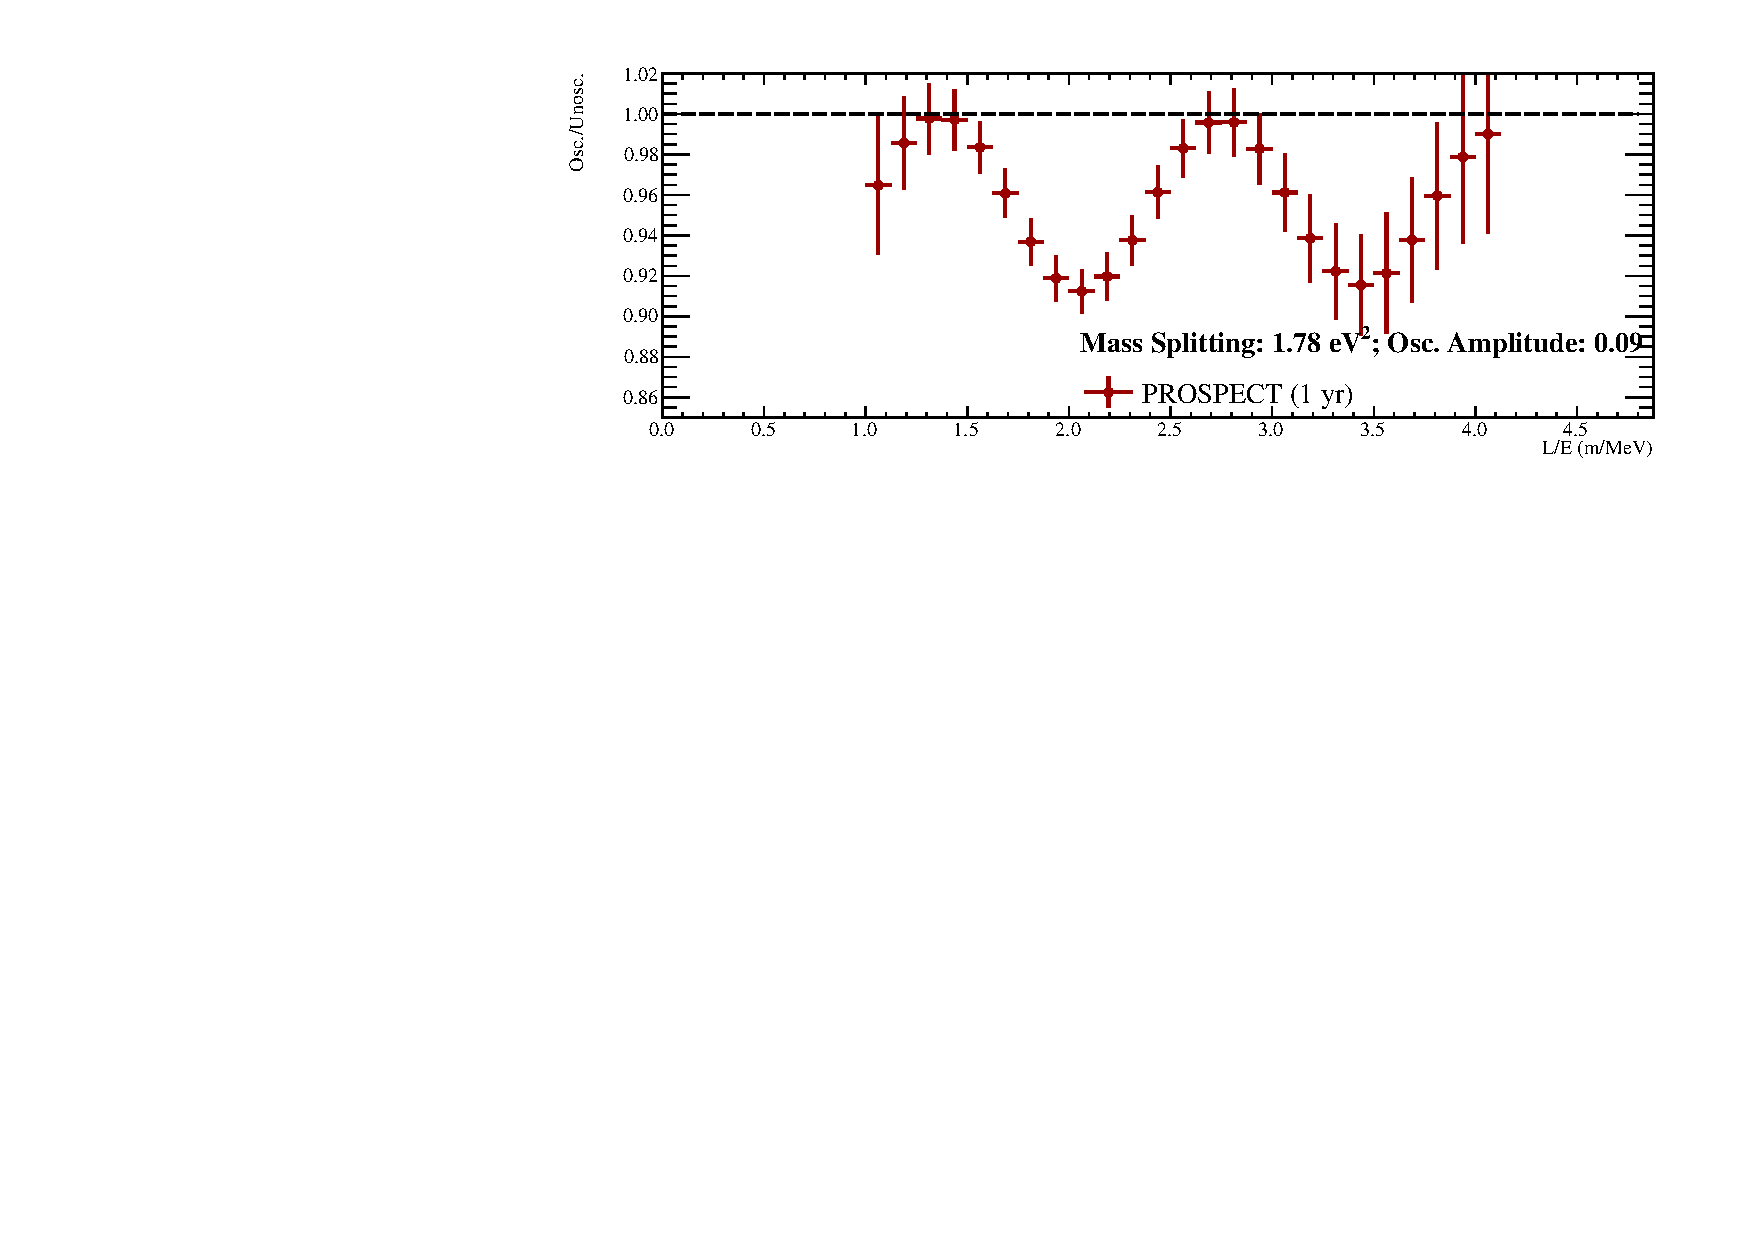
\includegraphics[width=0.7\linewidth]{tex/6-ac227-images/LoverE_1yr}
	\caption{The ratio of the oscillated to un-oscillated neutrino spectrum as a function of L/E that would be observed by PROSPECT after 1 year if a sterile neutrino signal was detected \cite{PSurukuchi:1534}.}
	\label{fig:lovere1yr}
\end{figure}
Given that the oscillation signal in PROSPECT is a deviation from an expected 1/$r^2$ neutrino rate fall-off with distance from the reactor, it is crucial to ensure that relative segment-to-segment volume variations do not mimic this signal.

Relative segment volumes can be measured via an event source uniformly distributed throughout the active volume of the detector. 
This was accomplished in PROSPECT by mixing a radioactive isotope, \Ac, with the liquid scintillator and using measured decay rates as a proxy for segment volume.

We chose \Ac for several reasons. First, because an \AaAa coincidence occurs in its decay chain, specifically $^{219}$Rn $\rightarrow ^{215}$Po + $\alpha \rightarrow ^{211}$Pb + \Aa, as highlighted in Figure~\ref{fig:ac227chain}.
\begin{figure}[!b]
	\centering
	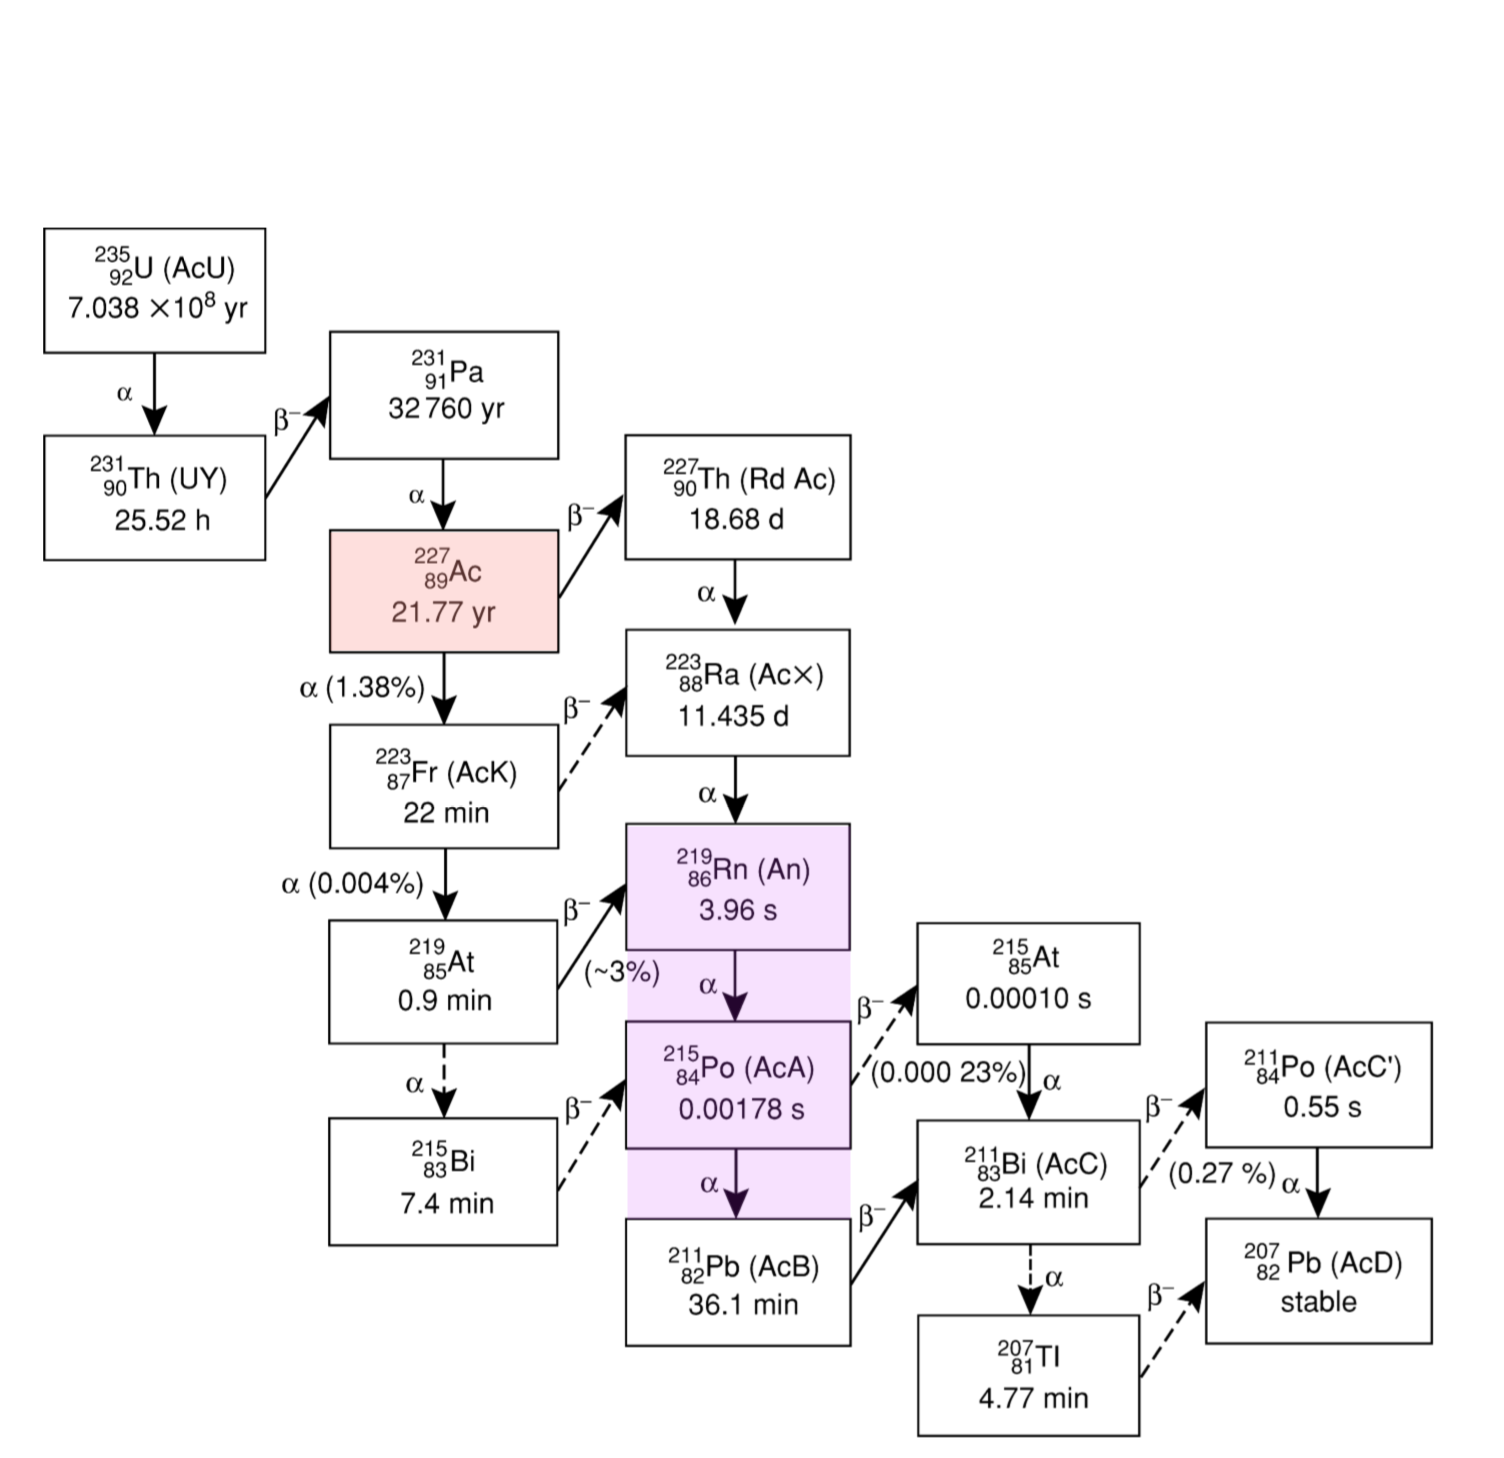
\includegraphics[width=0.6\linewidth]{tex/6-ac227-images/Ac227Chain}
	\caption{The full decay chain of \Ac (a daughter of $^{235}$U), in which the \AaAa coincidence of interest is highlighted \cite{Kirby2011}.}
	\label{fig:ac227chain}
\end{figure}
\Rn has a half-life of 3.96 $\pm$ 0.01 s and $\alpha$-decays 100\% of the time, while \Po has a half-life of 1.781 $\pm$ 0.005 ms and $\alpha$-decays  99.99977(2)\% of the time \cite{ENSDF}.
The \Aa decay of \Po (see Figure~\ref{fig:215poalphadecay}) is mono-energetic at 7.39 MeV which results in a $\sim$0.78 MeV$_{ee}$\footnote{Due to quenching in the scintillator that causes suppressed light output, the observed energy is sometimes referred to as electron-equivalent energy.} signal in the PROSPECT detector after quenching, well removed from nLi captures on $^6$Li (one half of the signal used for neutrino identification) that occur around 0.5 MeV$_{ee}$. 
In addition, there are no corresponding gammas with the \Po decay, making this a very clean and well defined signal.
The \Rn \Aa decays (see Figure~\ref{fig:219rnalphadecay}) are not as clean, with the alpha having a non-negligible probability of decaying to 3 excited states of the daughter in addition to the ground state and thus producing accompanying gamma rays, as listed in Table~\ref{tab:RnPoE}, but the use of time, energy, and PSD cuts make them easy to pair with corresponding \Po decays.

\begin{table}[!t]
	\centering
\begin{tabular}{|c|c|c|c|c|c|}
	\hline 
	& E$_\alpha$ [keV] & I$_\alpha$ \% &  & E$_\gamma$ [keV] & I$_\gamma$ \% \\ 
	\hline 
	\Rn & 6425.0(10) & 7.5(6) &  & 271.23(1) & 10.8(6) \\ 
	%\hline 
	& 6530(2) & 0.110(10) &  & 401.81(1) & 6.6(4) \\ 
	%\hline 
	& 6552.6(10) & 12.9(6) &  & 130.60(3) & 0.13(9) \\ 
	%\hline 
	& 6819.1(3) & 79.4(10) &  &  &  \\ 
	\hline 
	\Po & 7386.1(8) & 99.999770(20) &  &  &  \\ 
	\hline 
\end{tabular} 
\caption{Energy and absolute intensity of dominant $\alpha$ and $\gamma$ decay radiation for \Rn and \Po. Decay energies not listed here have an intensity of $< $0.05\%.}
\label{tab:RnPoE}
\end{table}

Another reason \Ac is an attractive source is its long half-life, 21.77 years, ensuring that the rate of RnPo\footnote{Short-hand used to refer to the event selection of the  $^{219}$Rn $\rightarrow ^{215}$Po + $\alpha \rightarrow ^{211}$Pb + \Aa chain} events remains close to constant over the lifetime of the detector.
It is also important that the chosen source is in equilibrium with its decay products at the time of use so that constant rates can be measured.
It takes about 188 days for \Ac to come into equilibrium with its decays products \cite{DBerish:597}, and given the probable amount of time that would pass between obtaining the source and adding it to the liquid scintillator in the detector, it was assumed that equilibrium would be reached. 

The ability to select RnPo events using a time coincidence analysis means that only a small amount of \Ac needs to be added to the liquid scintillator. 
This is important because PROSPECT cannot afford to introduce any extra background as it already has no overburden. 
It should also be noted that $\alpha$'s deposit their energy in the scintillator practically immediately, resulting in a highly localized signal. 
This also means that all RnPo events occur in the same segment, providing another handle that can be used in the event selection.

\begin{figure}[H]
	\centering
	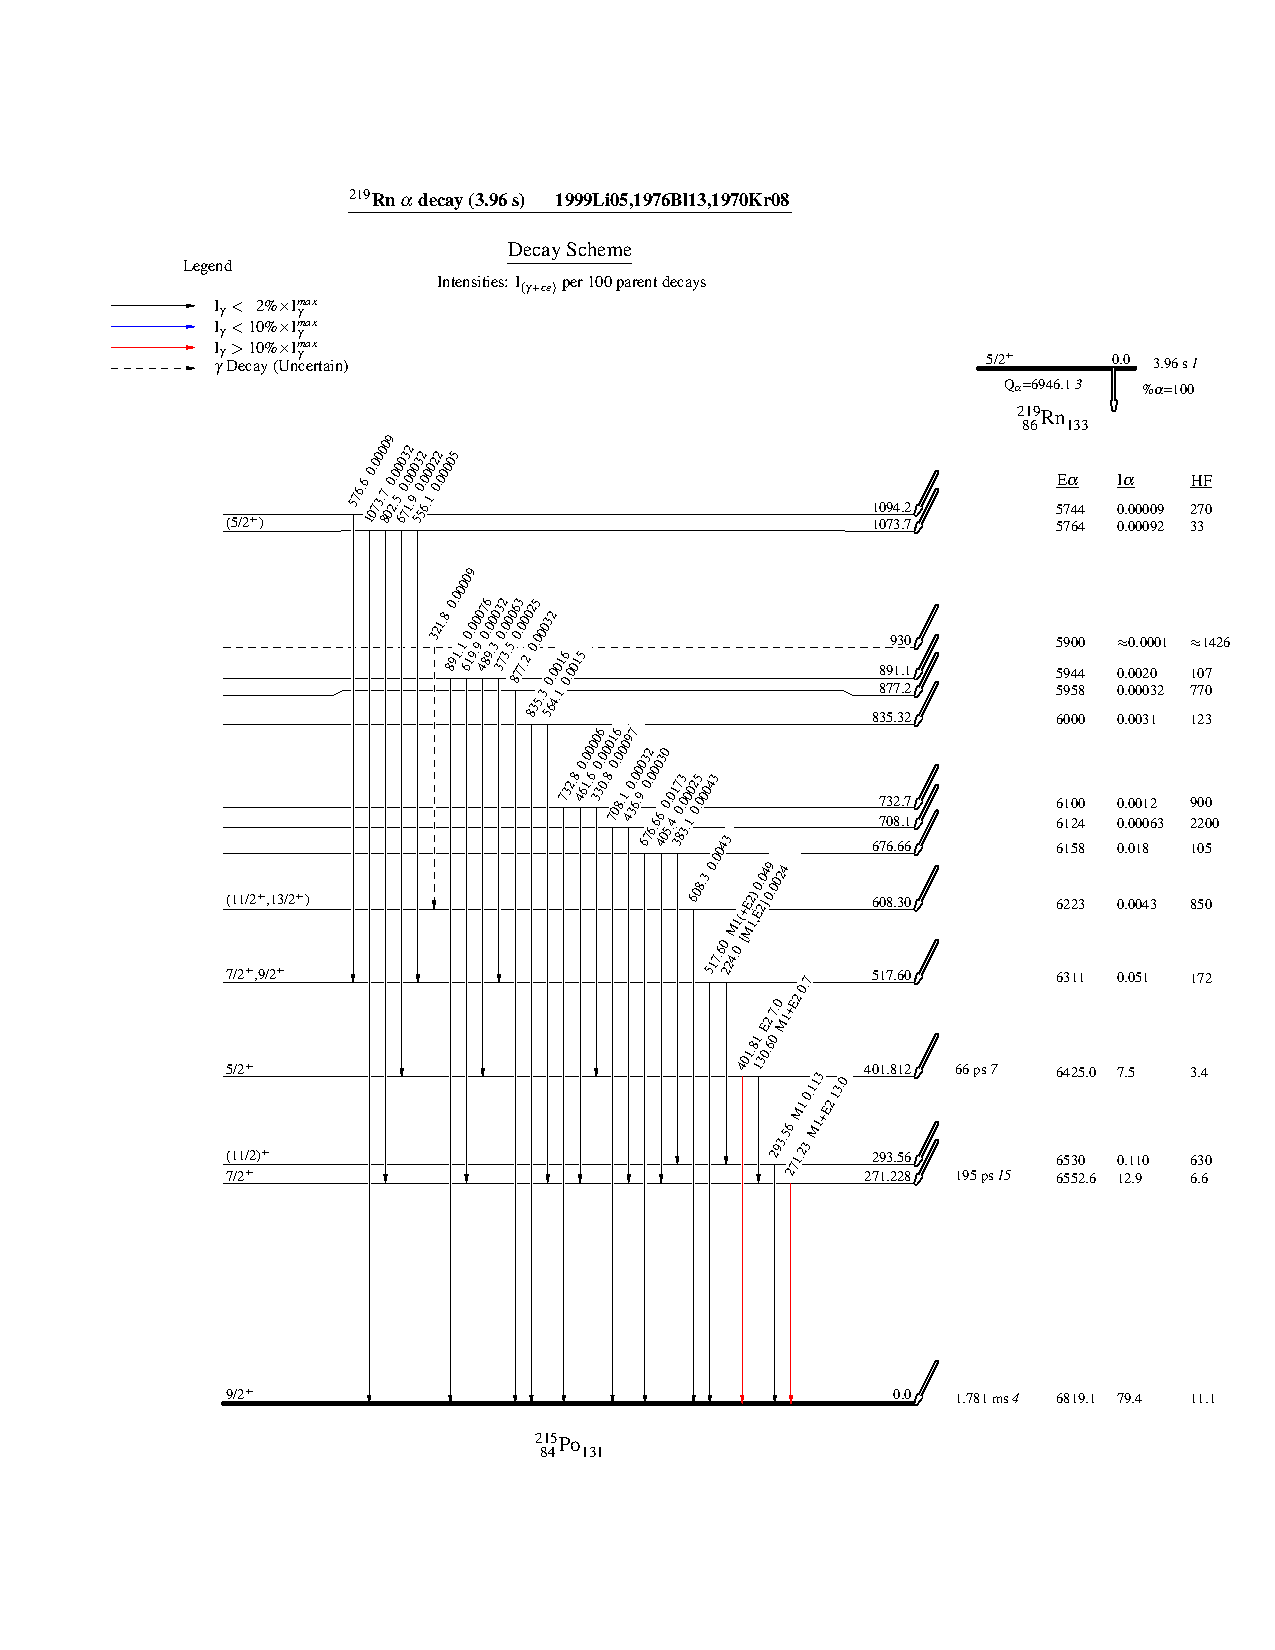
\includegraphics[width=0.9\linewidth]{tex/6-ac227-images/219RnAlphaDecay}
	\caption{The decay scheme of \Rn \cite{ENSDF}.}
	\label{fig:219rnalphadecay}
\end{figure}

\begin{figure}[H]
	\centering
	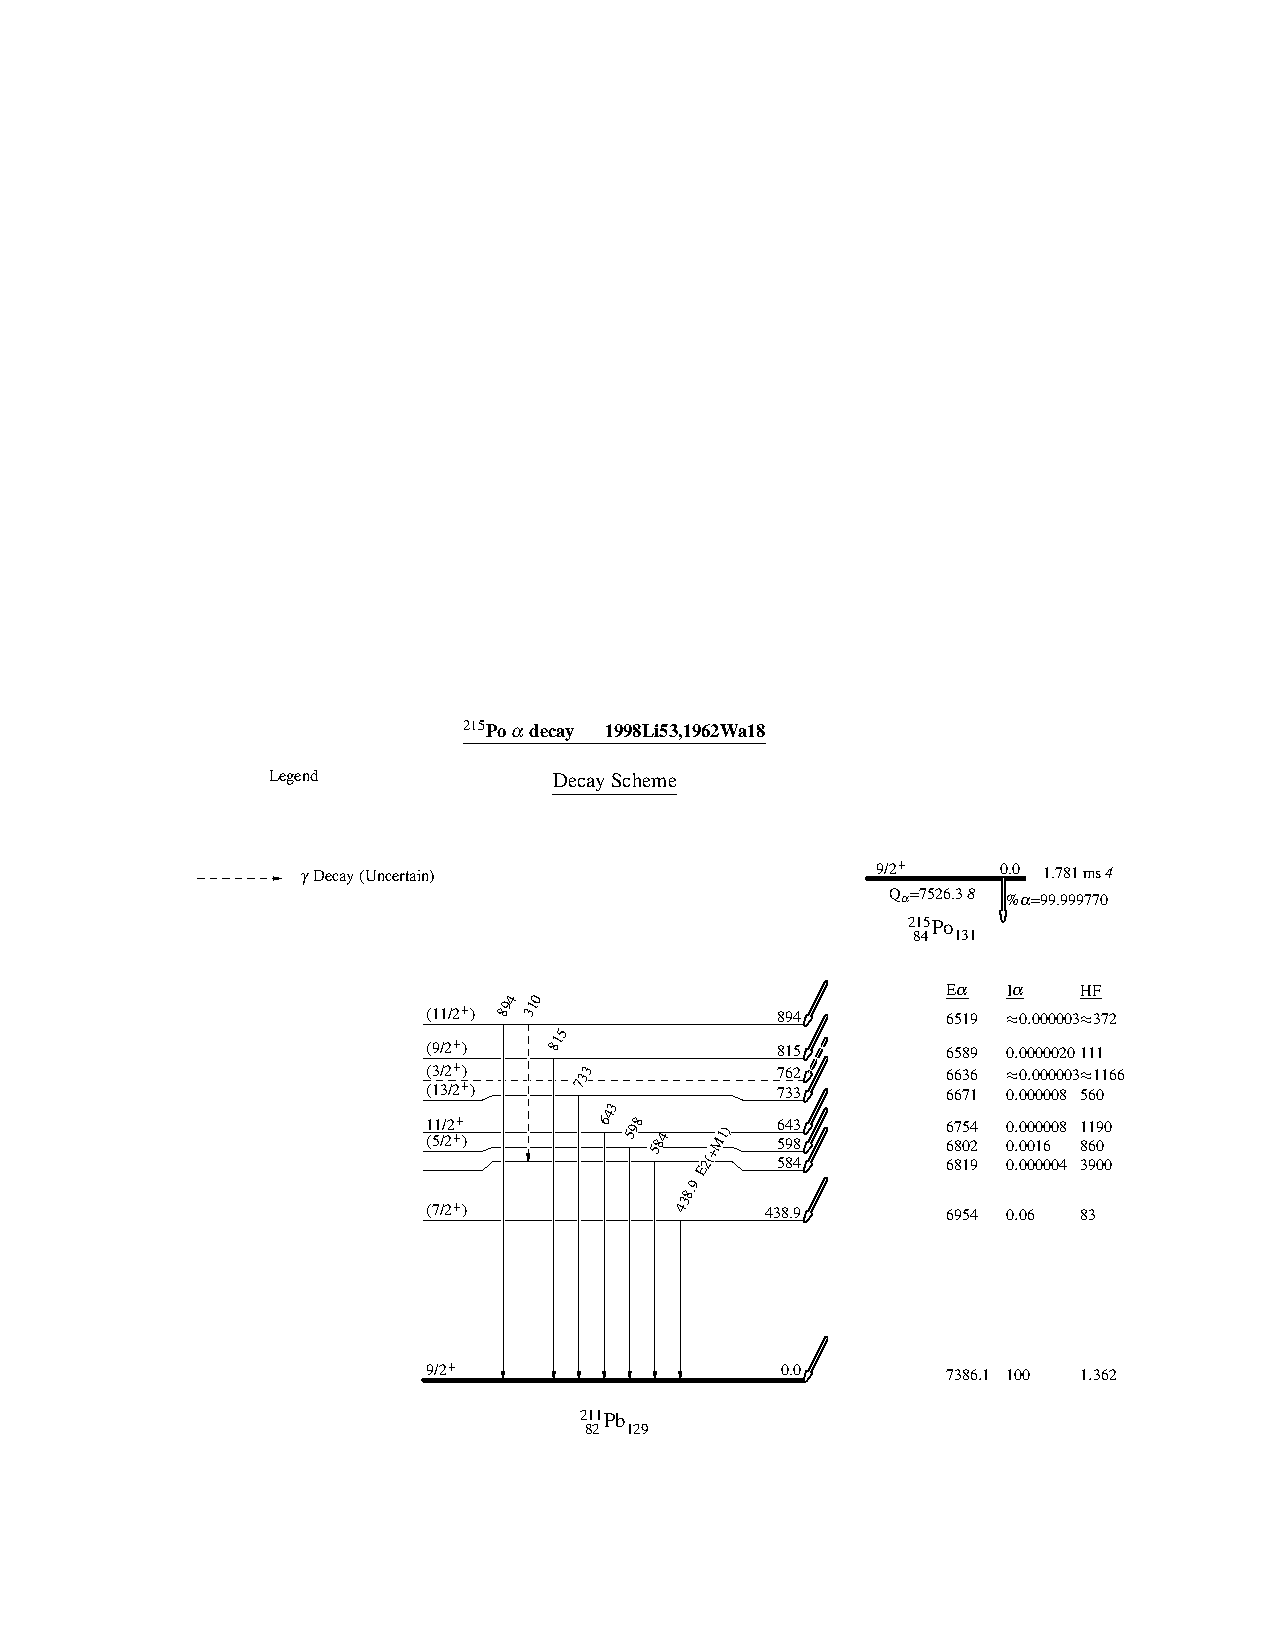
\includegraphics[width=0.9\linewidth]{tex/6-ac227-images/215PoAlphaDecay}
	\caption{The decay scheme of \Po \cite{ENSDF}.}
	\label{fig:215poalphadecay}
\end{figure}


\newpage
\section{Material Compatibility}

Before \Ac could be added to the PROSPECT detector, it had to be determined that \Ac and its daughters would not adsorb onto detector materials and that it would not degrade the scintillator.
If it was adsorbed then it would not be a uniform source in the detector, nullifying the ability to use measured decay rates as a proxy of volume.
To test this six material samples were placed in vials of identically prepared $^6$Li-LS spiked with $^{227}$Ac. The rate of \Ac in each sample vial and one reference vial with no material was measured and tracked over a period of 6 months. 
An observation of a significant decrease in rate, relative to the half-life of \Ac, would indicate that \Ac was adsorbing onto the material.

\subsection{Material and Scintillator Preparation}
The materials tested were: ultraviolet transmitting (UVT) acrylic, flourinated ethylene propylene (FEP), polylactide (PLA), polyether ether ketone (PEEK), a RG 188 cable, and viton o-rings. See Table~\ref{tab:materials} for a list of their uses in the detector and sample sizes.
To prepare the materials they were all placed in a single beaker with ultra-pure water and cleaned ultrasonically for 30 minutes.
They were then transferred to a watch glass and placed in a 50 C oven for two hours.
After drying they were placed in empty 12 mL vials.

The \Ac used to spike the scintillator was obtained from Eckert and Ziegler as a solution of 3.711$\times$10$^4$ Bq $\pm$ 1.32\% of \Ac in 10.22710 g of 1 M HCl, measured on September 6, 2016.
0.503 g of this solution was added to 192 g of $^6$Li-LS on December 15, 2016.
With an accepted half-life of 21.772 $\pm$ 0.003 yrs \cite{ENSDF}, the activity of the \Ac solution before adding to the LiLS was 36788 Bq, yielding a final activity of 94.2 Bq/10 g. 
This is the stock solution from which all LS was taken for the material studies and later on for spiking the detector.

Prior to filling all sample vials the threads of each vial were wrapped with teflon tape in an effort to obtain a secure seal. 
The reference vial was filled on December 15, 2016 with 10.030 g of \Ac spiked LiLS from the stock solution, yielding an expected activity of 94.5 Bq.
All material vials were filled on February 24, 2017 with the amount of stock solution added to each listed in Table~\ref{tab:MatFill}.
At the time of filling the rate in each vial was expected to be $\sim$93 Bq.
For a photograph of all filled material sample vials see Figure~\ref{fig:samples}.

\begin{table}[h]
	\centering
\begin{tabular}{|p{0.16\textwidth}|p{0.4\textwidth}|p{0.33\textwidth}|}
	\hline 
	\textbf{Material} & \textbf{Detector Use} & \textbf{Sample Size} \\ 
	\hline 
	UVT Acrylic & Front window of PMT housing & 1.0 $\times$ 1.15 $\times$ 0.1 cm$^3$ \\ 
	\hline 
	FEP  & Film on optical separators & 1.5 $\times$ 1.5 cm$^2$, 3 mm thick \\ 
	\hline 
	PLA & 3D printed pinwheels & 10 disks; 0.5 cm diameter, 0.1 cm thick \\ 
	\hline 
	PEEK & Seal plugs through which the high voltage and signal cables were threaded. Screws used to bolt together segment supports. Spacers at the base of the acrylic tank. & 1 Nut; ID 0.5 cm, small OD 1cm, large OD 1.1cm, thickness 0.5 cm \\ 
	\hline 
	RG188 Cable & High voltage and signal cables & 4.5'' long \\ 
	\hline 
	Viton O-ring & Seal back plugs of PMT housings and seal acrylic tank & 10 O-rings; OD 6mm, ID ~3mm, thickness 1.5mm \\ 
	\hline 
\end{tabular} 
\caption{Samples used to test if \Ac or its daughters would adsorb onto detector materials.}
\label{tab:materials}
\end{table}

\begin{table}[h]
	\centering
\begin{tabular}{|c|c|c|}
	\hline 
	\textbf{Material} & \textbf{Date Filled} & \textbf{LiLS Added (g)}  \\ 
	\hline 
	Reference & 12/15/2016 & 10.030 \\ 
	\hline 
	UVT Acrylic & \multirow{6}{*}{02/24/2017}  & 9.98 \\ 
	%\hline 
	FEP &  & 9.98 \\ 
	%\hline 
	PLA &  & 9.999 \\ 
	%\hline 
	PEEK &  & 9.99 \\ 
	%\hline 
	RG188 Cable &  & 9.981  \\ 
	%\hline 
	Viton O-ring &  & 10.011  \\ 
	\hline 
\end{tabular} 
\caption{The weight of \Ac spiked LiLS that was added to each sample vial.}
\label{tab:MatFill}
\end{table}

\begin{figure}[H]
	\centering
	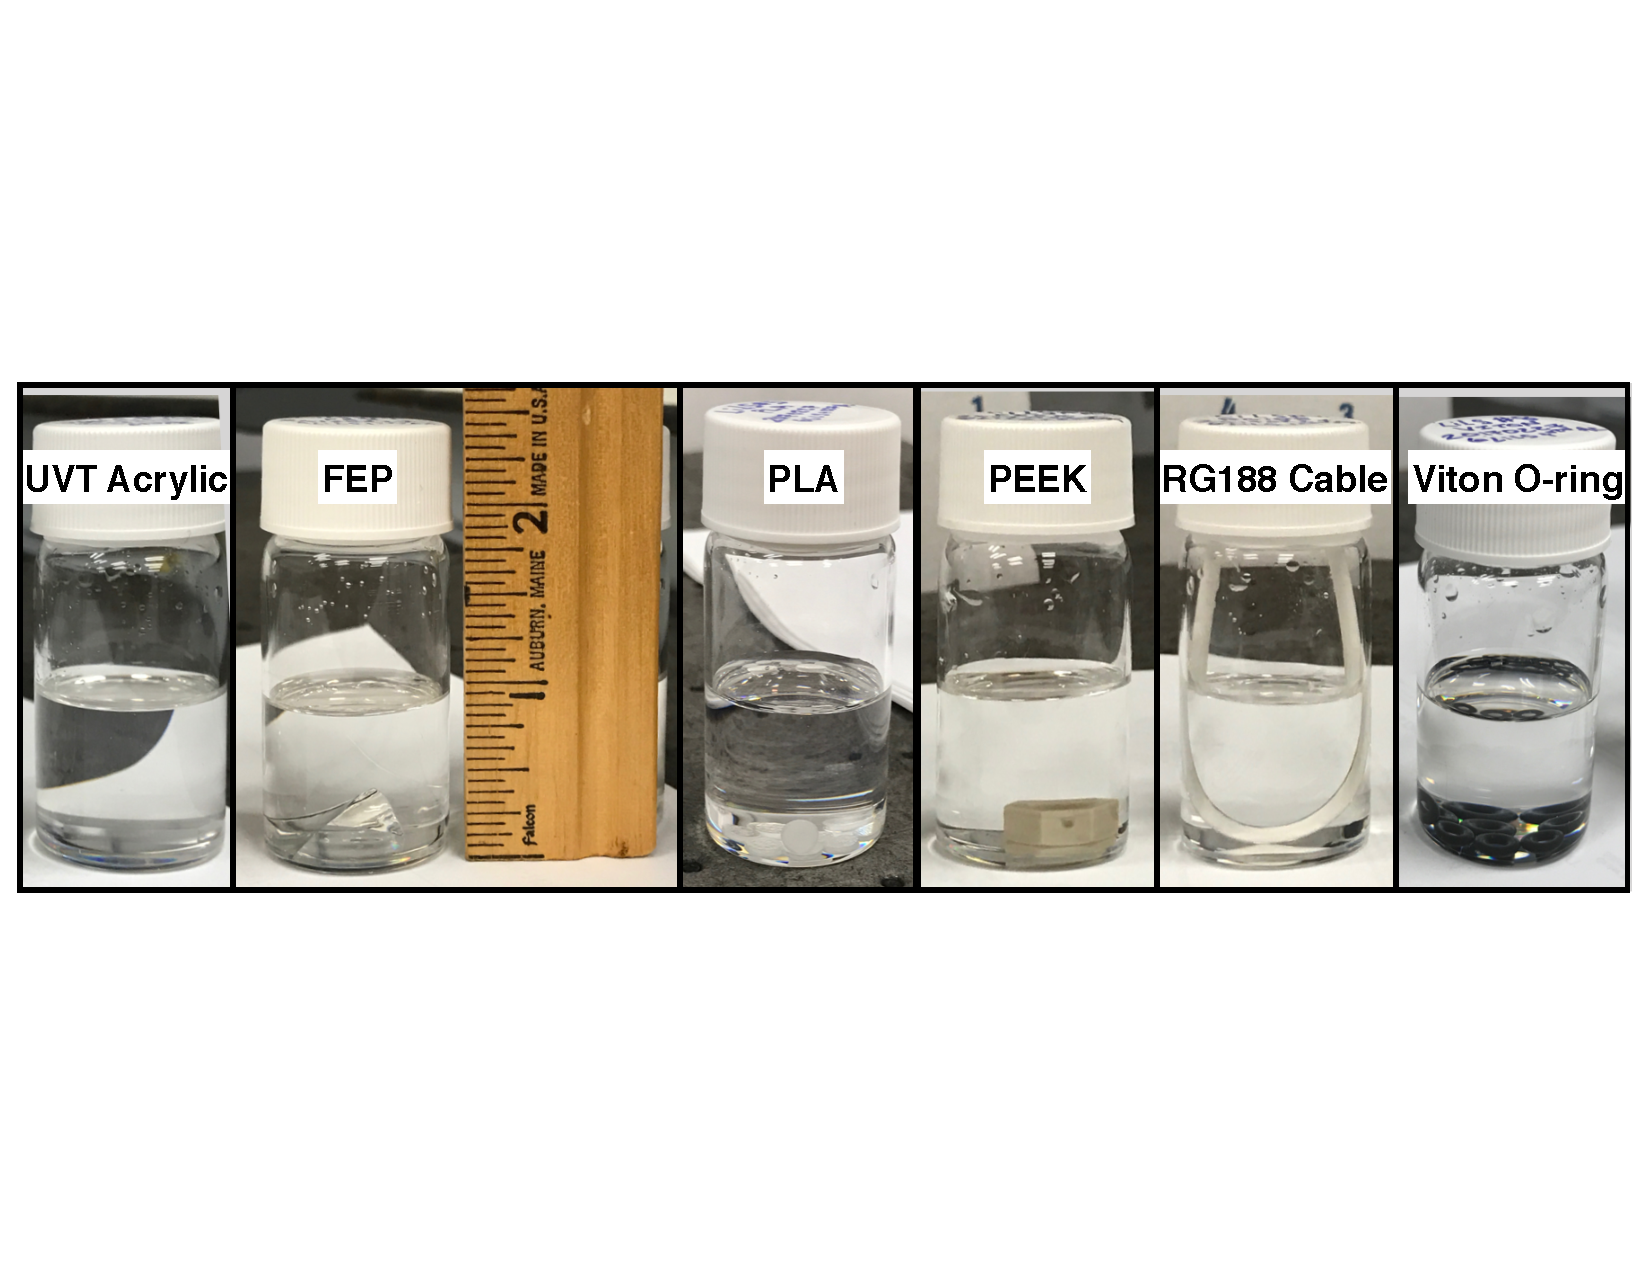
\includegraphics[width=0.8\linewidth]{tex/6-ac227-images/BNL/Samples}
	\caption{Photos of all material sample vials filled with \Ac spiked LiLS, with ruler for scale.}	
	\label{fig:samples}
\end{figure}

\subsection{Detector}

The detector consisted of a 2-inch photomultiplier tube coupled using optical grease to a solid cylinder of UVT acrylic painted with reflective white paint with an insert cut out to hold the sample vials, as shown in Figure~\ref{fig:blackbox}.
Placed in a dark box the PMT was cabled to a CAEN DT55xx Desktop HV Power Supply and a CAEN DT5730 8 Channel 14-bit 500 MS/s Digitizer \cite{CAENDigit}.
A modified version of Wavedump 3.7.2 \cite{CAENWD} was used to start and stop the data runs and save the waveforms of the signals.

\begin{figure}[H]
	\centering
	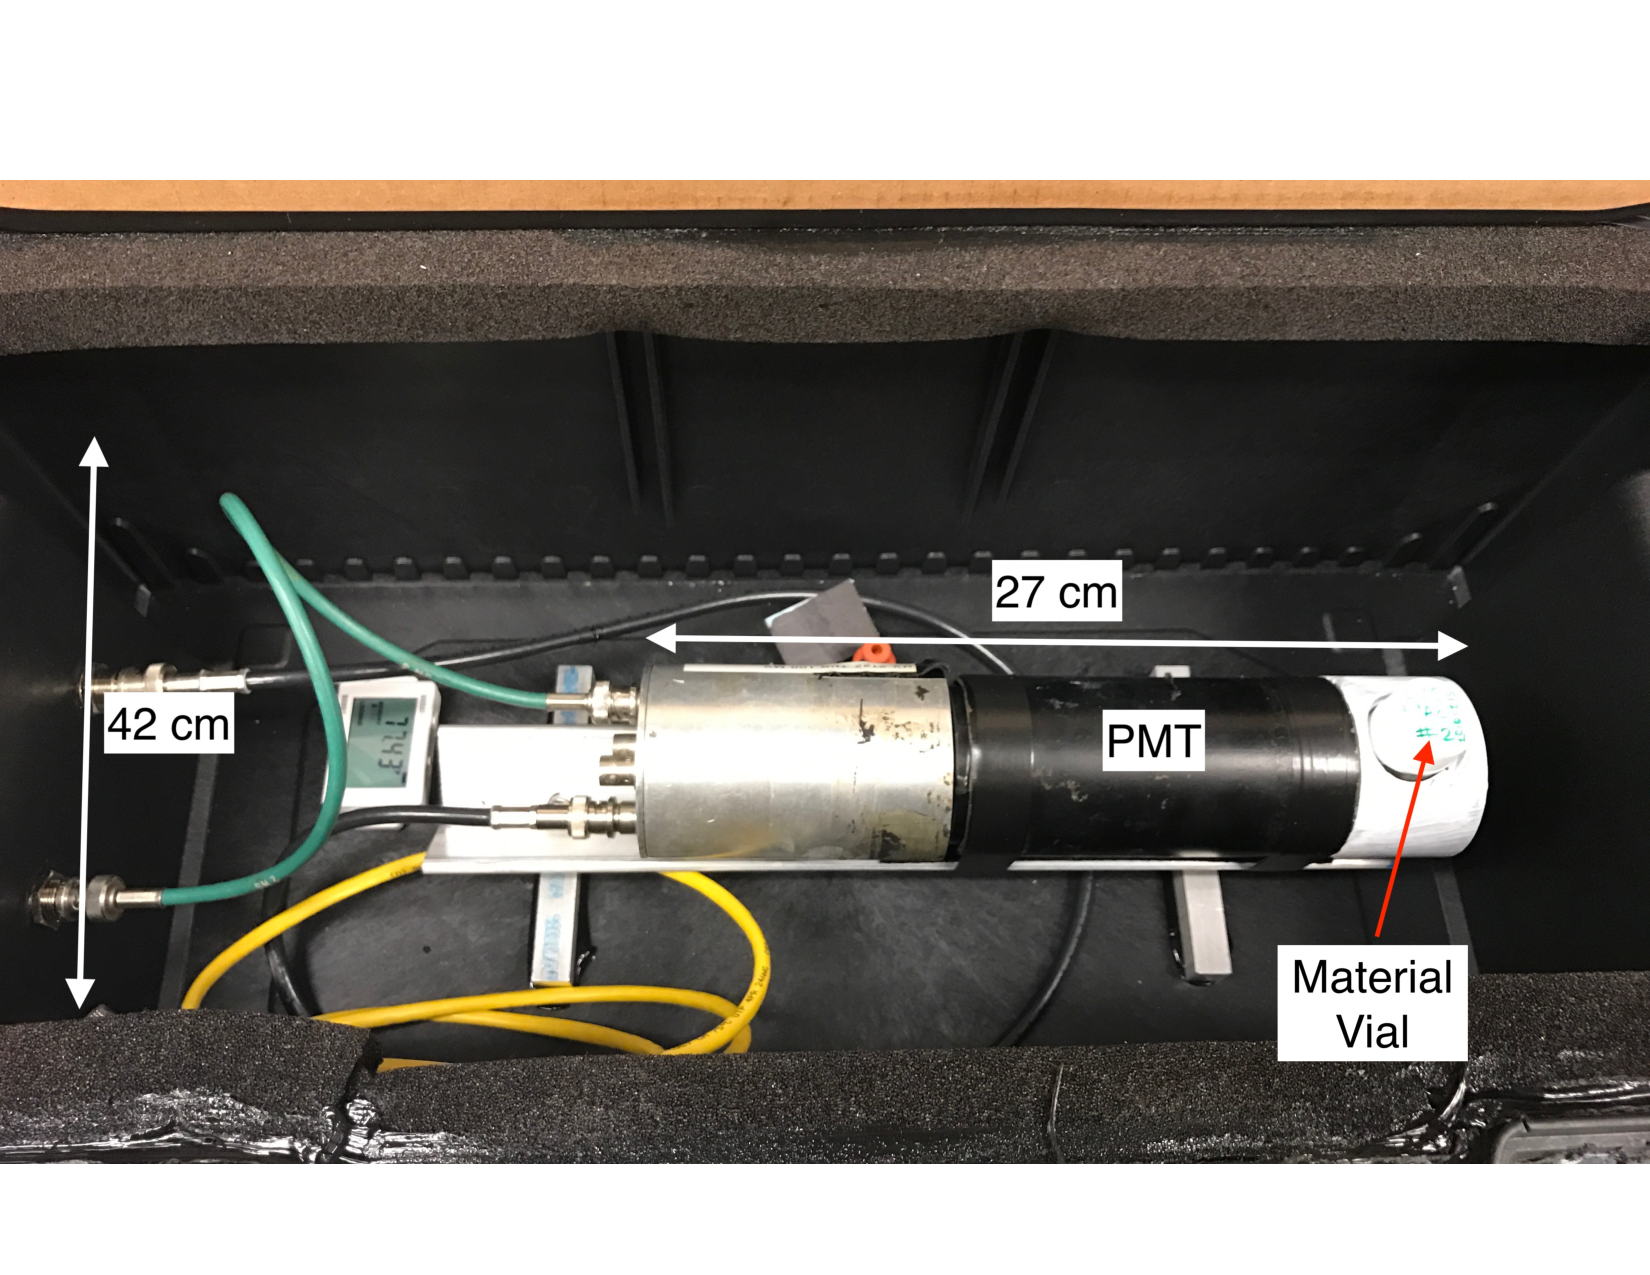
\includegraphics[width=0.65\linewidth]{tex/6-ac227-images/BNL/BlackBox}
	\caption{Detector used for material studies, consisting of a 2-inch PMT coupled to an acrylic cylinder holding the sample vials, all contained in a dark box. The PMT is cabled to a power supply and digitizer that exist outside of the box.}
	\label{fig:blackbox}
\end{figure}

\subsection{Data Analysis}

The raw waveforms were analyzed to calculate the energy and PSD of each signal. 
Each collected waveform consisted of 250 2 ns samples.
The energy was measured by taking the integral of the waveform using the trapezoidal rule in ADC units.
The total energy was converted to nC using
\begin{equation}
E[nC] = E[ADC] \times \frac{1\times10^9}{R\times\textrm{sample-rate}\times n[ADC/V]}
\end{equation}
where $R$, the resistance, is 50 $\Omega$, the sample-rate is $5\times10^8$ Hz, and $n = (2^{14} -1)/2 = 8191.50$ ADC/V, because we used a 14 bit ADC with a 2 V range.
The tail and total fractions used to calculate the PSD were both measured from the leading half-minimum point of the negative pulses.
The total pulse area was measured as the integral from 10 samples before the half-min to 140 samples after.
The tail area was measured as the integral from 19 samples after the half-max to 140 samples after.
For an example of this for a typical alpha signal in the reference sample see Figure~\ref{fig:waveformbnl}.

\begin{figure}[!t]
	\centering
	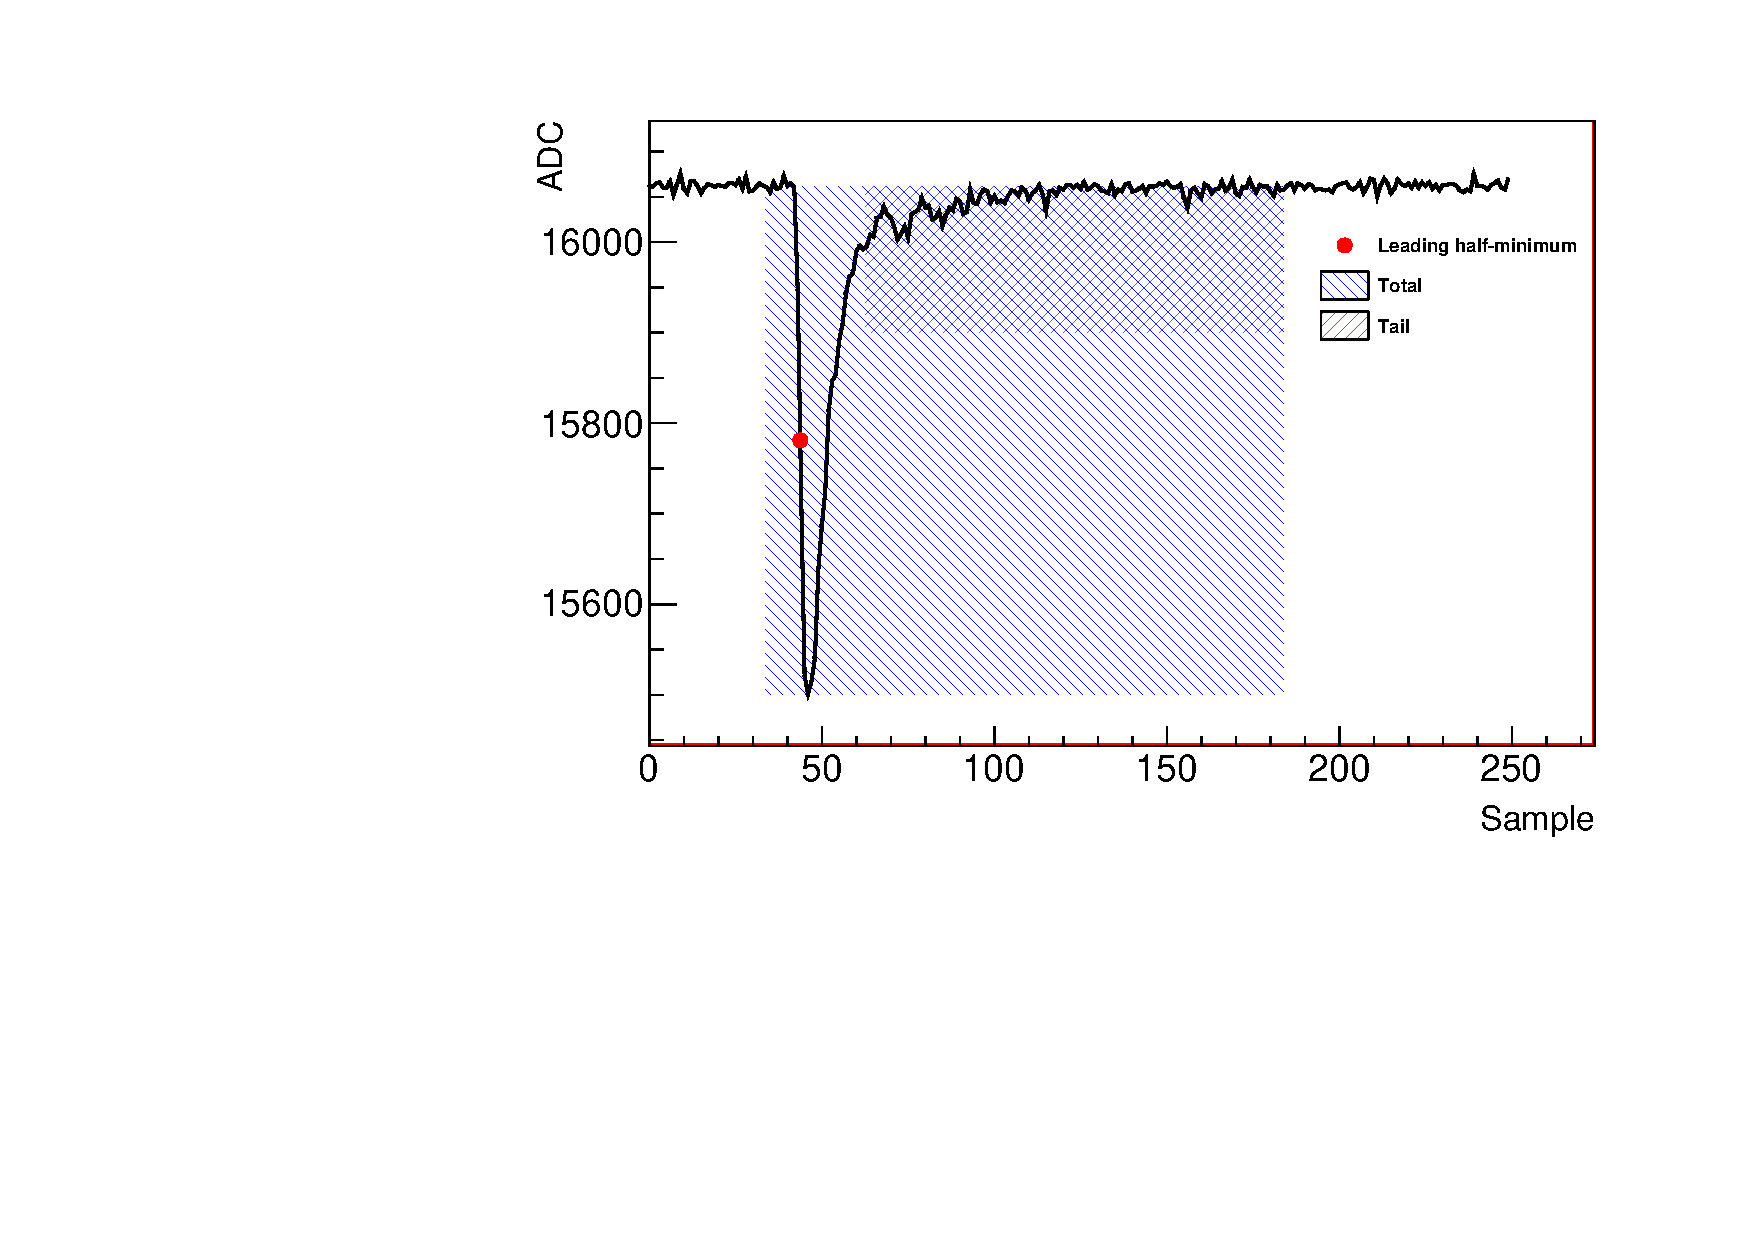
\includegraphics[width=0.6\linewidth]{tex/6-ac227-images/BNL/Waveform_BNL}
	\caption{A typical waveform for an alpha event in the reference sample. The leading half-minimum (circle, red) determines the windows for total pulse area (blue) and tail area (magenta).}
	\label{fig:waveformbnl}
\end{figure}

The \Ac coincident alpha events, labeled RnPo events for the remainder of this document, were found by applying a set of timing, energy, and PSD cuts along with an accidental background subtraction.
Po events were found first by applying the energy and PSD cuts listed in Table~\ref{tab:MatCuts}. 
Rn coincidental events were found by looking in a 12.85 ms time window before a given Po event and applying the same energy and PSD cuts.
This time window was 5 times the lifetime of Po, 2.57 ms, allowing for the collection of all possible coincident events.
Accidental events were found by looking in the same length time window, using the same energy and PSD cuts, but offset 10 Po lifetimes before a given Po event.
RnPo events were then measured by subtracting the accidental events from the coincident events.
See Figure~\ref{fig:rnpoenpsd} for an example of typical energy and PSD distributions in the reference sample.
\begin{table}[H]
	\centering
	\begin{tabular}{c|c}
		\hline 
		Energy & 0.01 $<$ E $<$ 0.055 nC \\ 
		\hline 
		PSD & 0.31 $<$ PSD $<$ 1.0  \\ 
		\hline 
		$\Delta$t = t$_{\mathrm{delay}}$ - t$_{\mathrm{prompt}}$ & $\Delta$t $<$ 5$\tau_{\textrm{Po}}$ \\ 
		\hline 
	\end{tabular} 
	\caption{Energy, PSD, and time cuts used to find RnPo events where $\tau_{\textrm{Po}}=2.57~\textrm{ms}$. Energy and PSD cuts are applied to both prompt and delay events.}
	\label{tab:MatCuts}
\end{table}

\begin{figure}[!t]
	\centering
	\begin{subfigure}{0.5\linewidth}
		\centering
		\includegraphics[width=1.\linewidth]{"tex/6-ac227-images/BNL/RnPoEn_TimeBin23_S2"}
		\caption{}
	\end{subfigure}%
	\begin{subfigure}{0.5\linewidth}
		\centering
		\includegraphics[width=1.\linewidth]{"tex/6-ac227-images/BNL/RnPoPSD_TimeBin23_S2"}
		\caption{}
	\end{subfigure}
	\caption{Typical energy (a) and PSD (b) distributions for 3.4 livetime-hours of RnPo events in the reference sample after accidental background subtraction.}
	\label{fig:rnpoenpsd}
\end{figure}

The rate of RnPo events was then determined by fitting the RnPo $\Delta t$ distribution with
\begin{equation}
	f(t) = N_0e^{-t/\tau}
	\label{eq:MatDtFit}
\end{equation}
where $N_0$ and $\tau$, the lifetime of \Po (accepted as 2.569$\pm$0.007 ms), are allowed to vary. 
Using the fit results, the rate was then defined as
\begin{equation}
	R = \frac{N_0 \tau}{\textrm{bin-width}\times\textrm{livetime}}
\end{equation}
\begin{equation}
	\sigma_R = R \times \sqrt{  \left(\frac{\sigma_{N_0}}{N_0}\right)^2 + \left(\frac{\sigma_{\tau}}{\tau}\right)^2 + \frac{2\sigma_{N_{0}\tau}}{N_0\tau} }
\end{equation}
where the livetime was measured, for each run, as the time from the beginning of the run to the last Po event. 
An example of a typical RnPo $\Delta t$ distribution can be seen in Figure~\ref{fig:rnpodttimebin23s2}, where fitting $\Delta t$ with Equation~\ref{eq:MatDtFit} resulted in a \Po lifetime of 2.58$\pm$0.02 ms that agrees well with the accepted value of 2.569$\pm$0.007 ms. It should be noted here that the energy and PSD cuts were made wide enough so that no efficiency correction needed to be applied.

\begin{figure}[H]
	\centering
	\includegraphics[width=1.\linewidth]{"tex/6-ac227-images/BNL/RnPoDt_TimeBin23_S2"}
	\caption{A typical example of the RnPo $\Delta t$ distributions for the 3.4 livetime-hours of events in the reference sample. Left: coincidental and accidental distributions found using the defined energy and PSD cuts. Right: the $\Delta t$ distribution after subtraction of the accidental distribution, fit with Equation~\ref{eq:MatDtFit}.}
	\label{fig:rnpodttimebin23s2}
\end{figure}

\subsection{Results}

The RnPo rate was calculated for each material sample and the reference sample over a period of about six months. These results can be seen in Figure~\ref{fig:ratevstimeallsamples}.
Though statistical errors vary from around 0.6-1\%, overall rates fluctuate by as much as $\pm8\%$ about the mean, indicating the size of unaccounted for systematic errors.

\begin{figure}[!b]
	\centering
	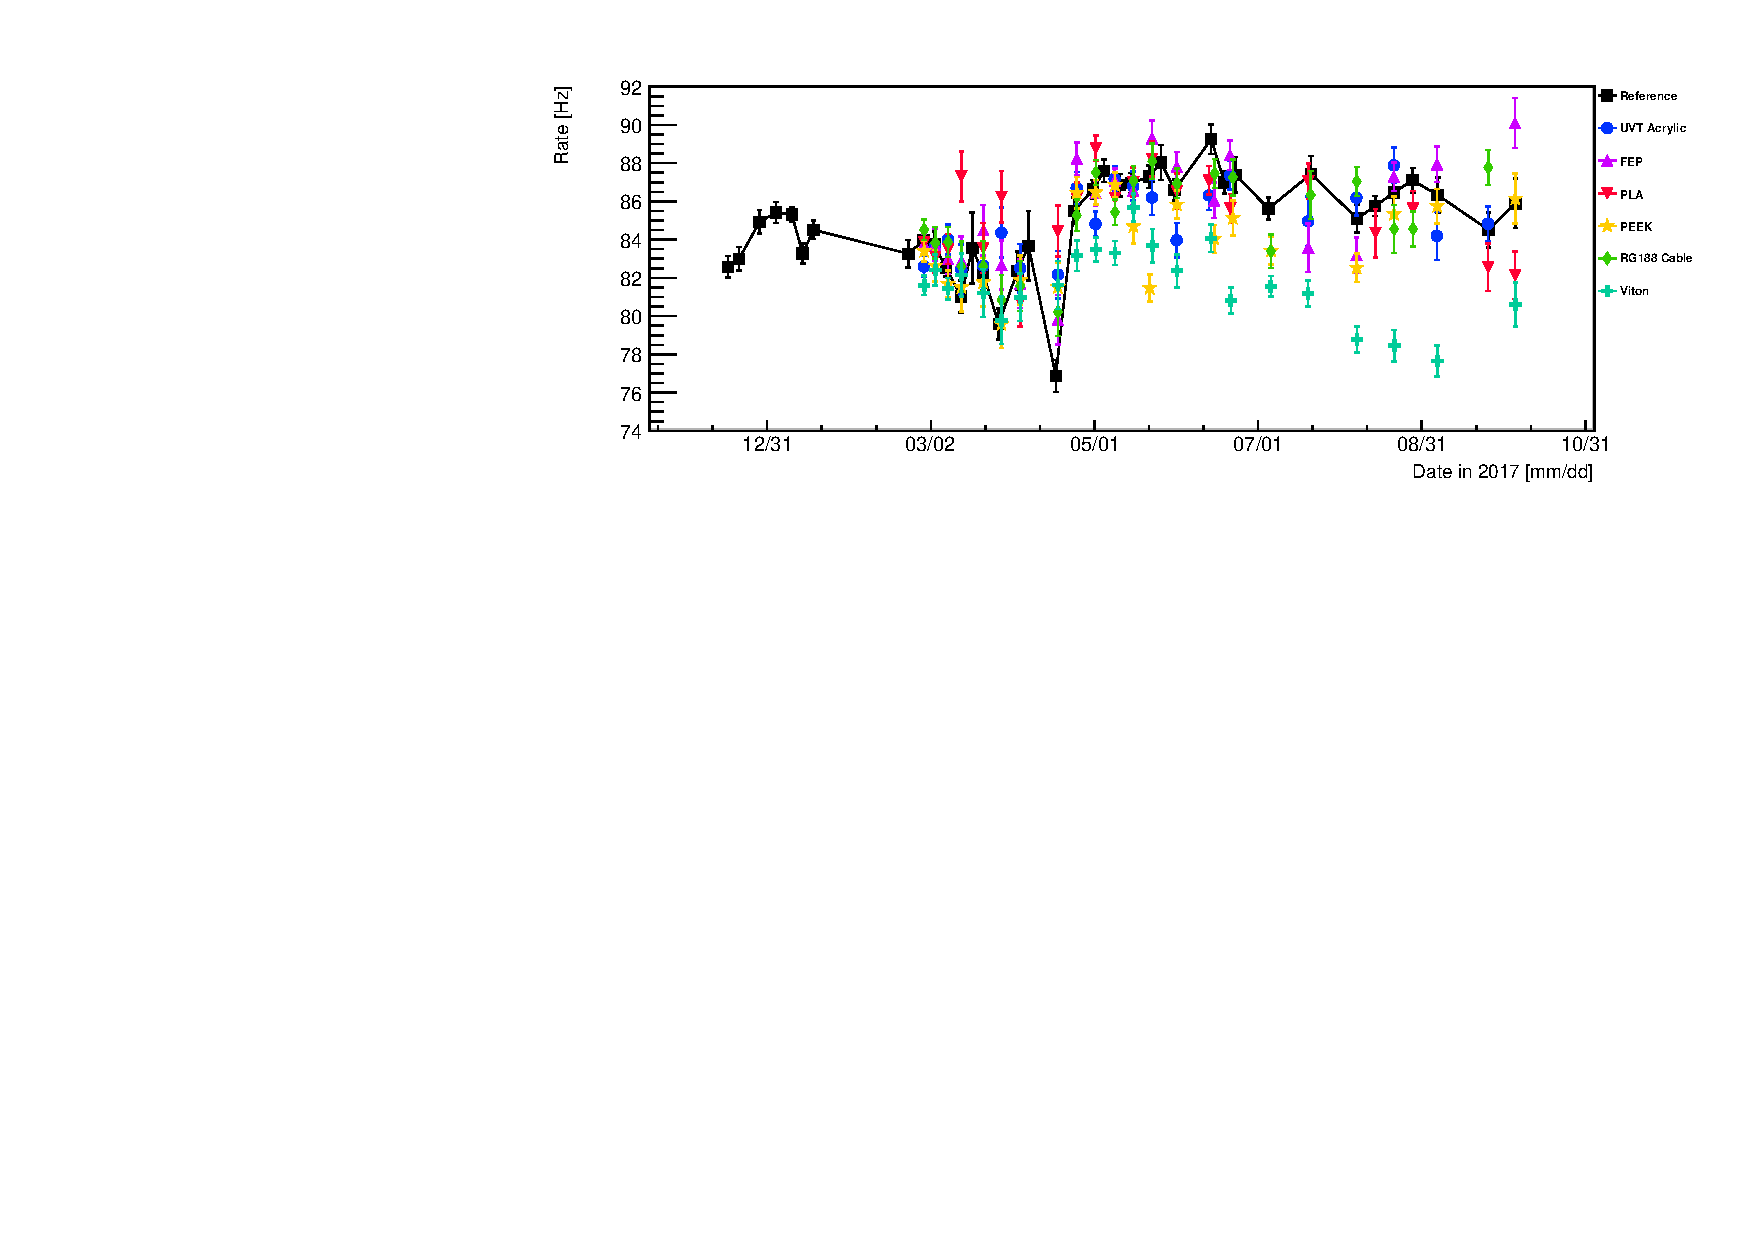
\includegraphics[width=1\linewidth]{tex/6-ac227-images/BNL/RateVsTime_AllSamples}
	\caption{\Ac rate for each material sample. Errors are statistical.}
	\label{fig:ratevstimeallsamples}
\end{figure}

Systematic variations can be better understood by looking at the behavior of the \Po energy distribution through time.
This was done by fitting this distribution for the reference sample with a sum of two Gaussians to account for the non-Gaussian nature of the peak as demonstrated in Figure~\ref{fig:poenfittimebin23s2}.
The mean and 1$\sigma$ width of each of these Gaussians versus time is shown in Figures~\ref{fig:poenmeanvstimes2} and ~\ref{fig:poenwidthvstimes2}.
It can be seen that the \Po energy mean varies about 5\% and the width around 15\%.

\begin{figure}[h]
	\centering
	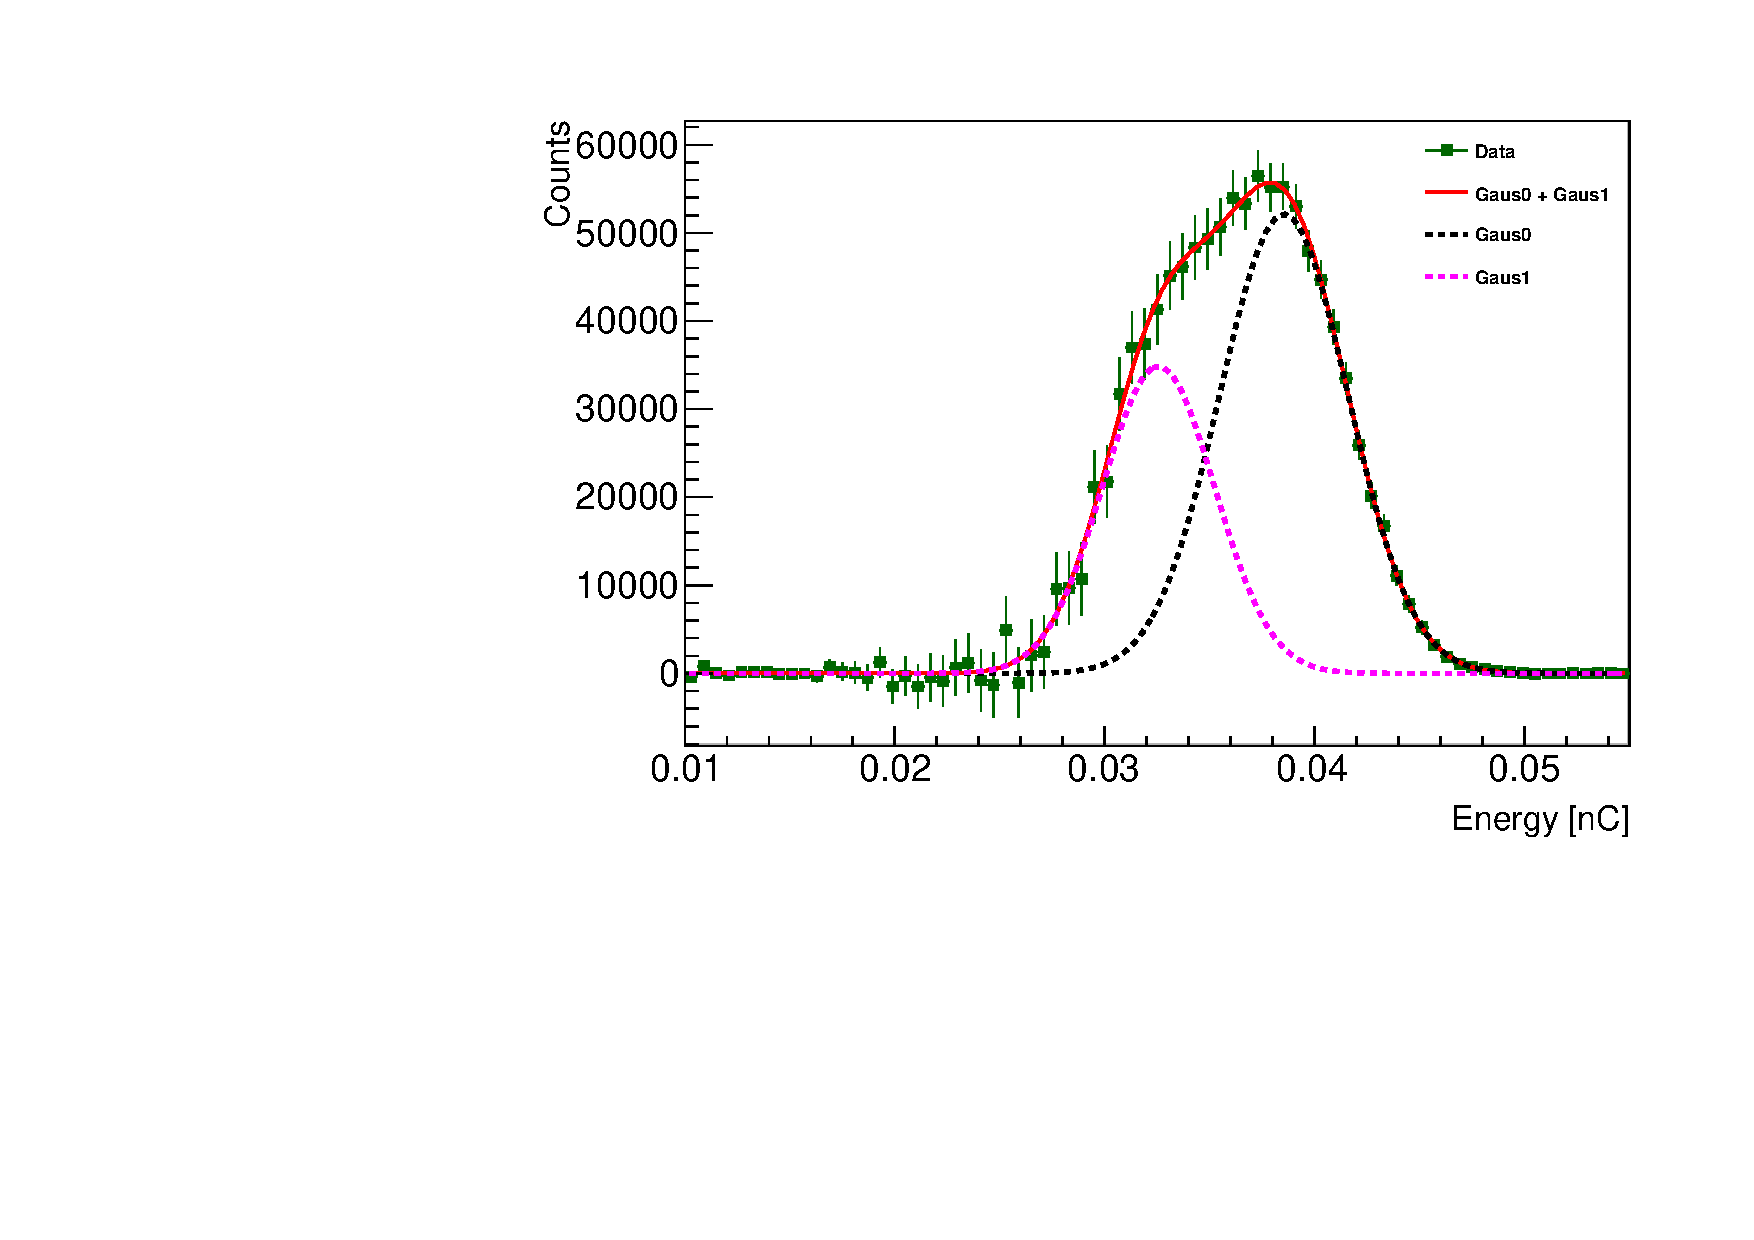
\includegraphics[width=0.6\linewidth]{tex/6-ac227-images/BNL/PoEnFit_TimeBin23_S2}
	\caption{\Po energy distribution for the reference sample, fit with a sum of two Gaussians. The total fit is seen in red, while the two Gaussians are drawn as the pink and black dashed lines.}
	\label{fig:poenfittimebin23s2}
\end{figure}

\begin{figure}[H]
	\centering
	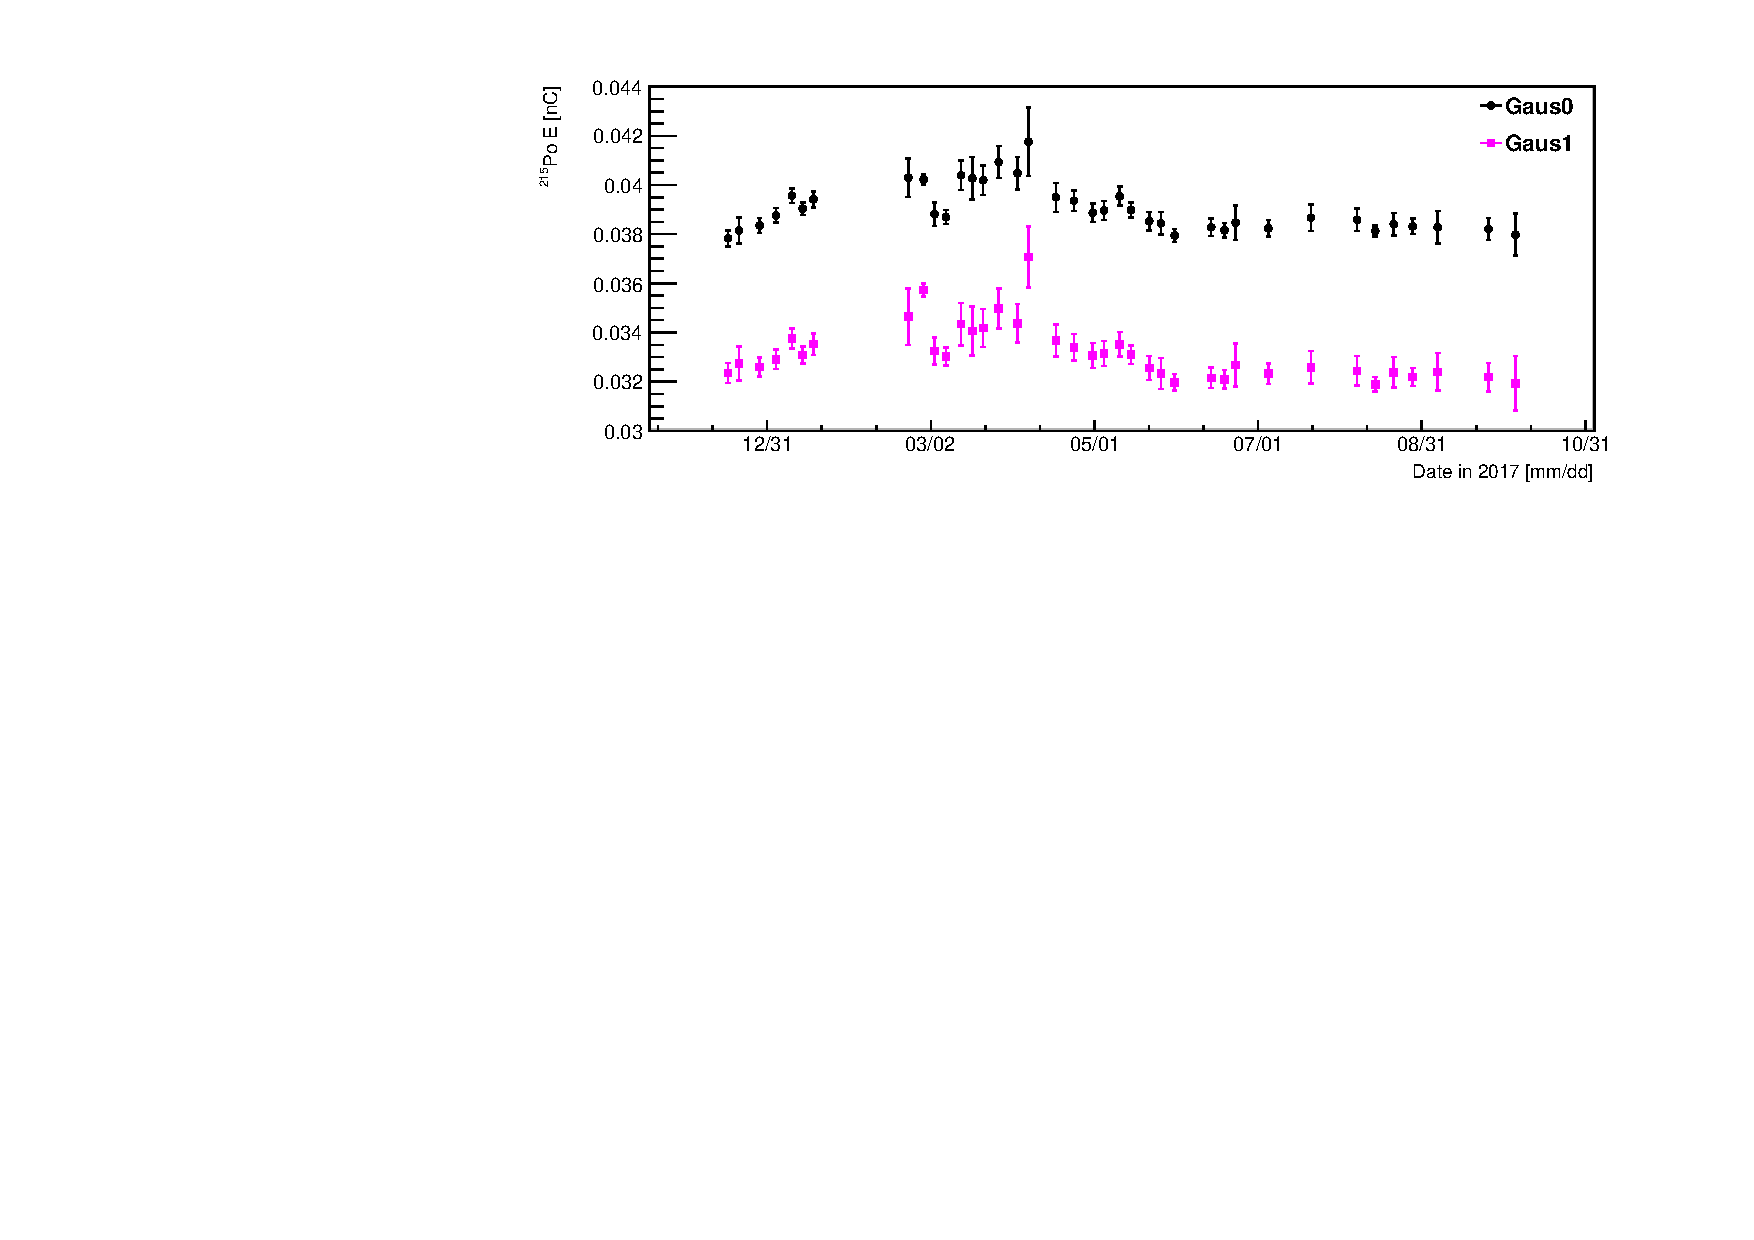
\includegraphics[width=0.9\linewidth]{tex/6-ac227-images/BNL/PoEnMeanVsTime_S2}
	\caption{The mean of the two Gaussians fit to the \Po energy distribution for the reference sample.}
	\label{fig:poenmeanvstimes2}
\end{figure}

\begin{figure}[h]
	\centering
	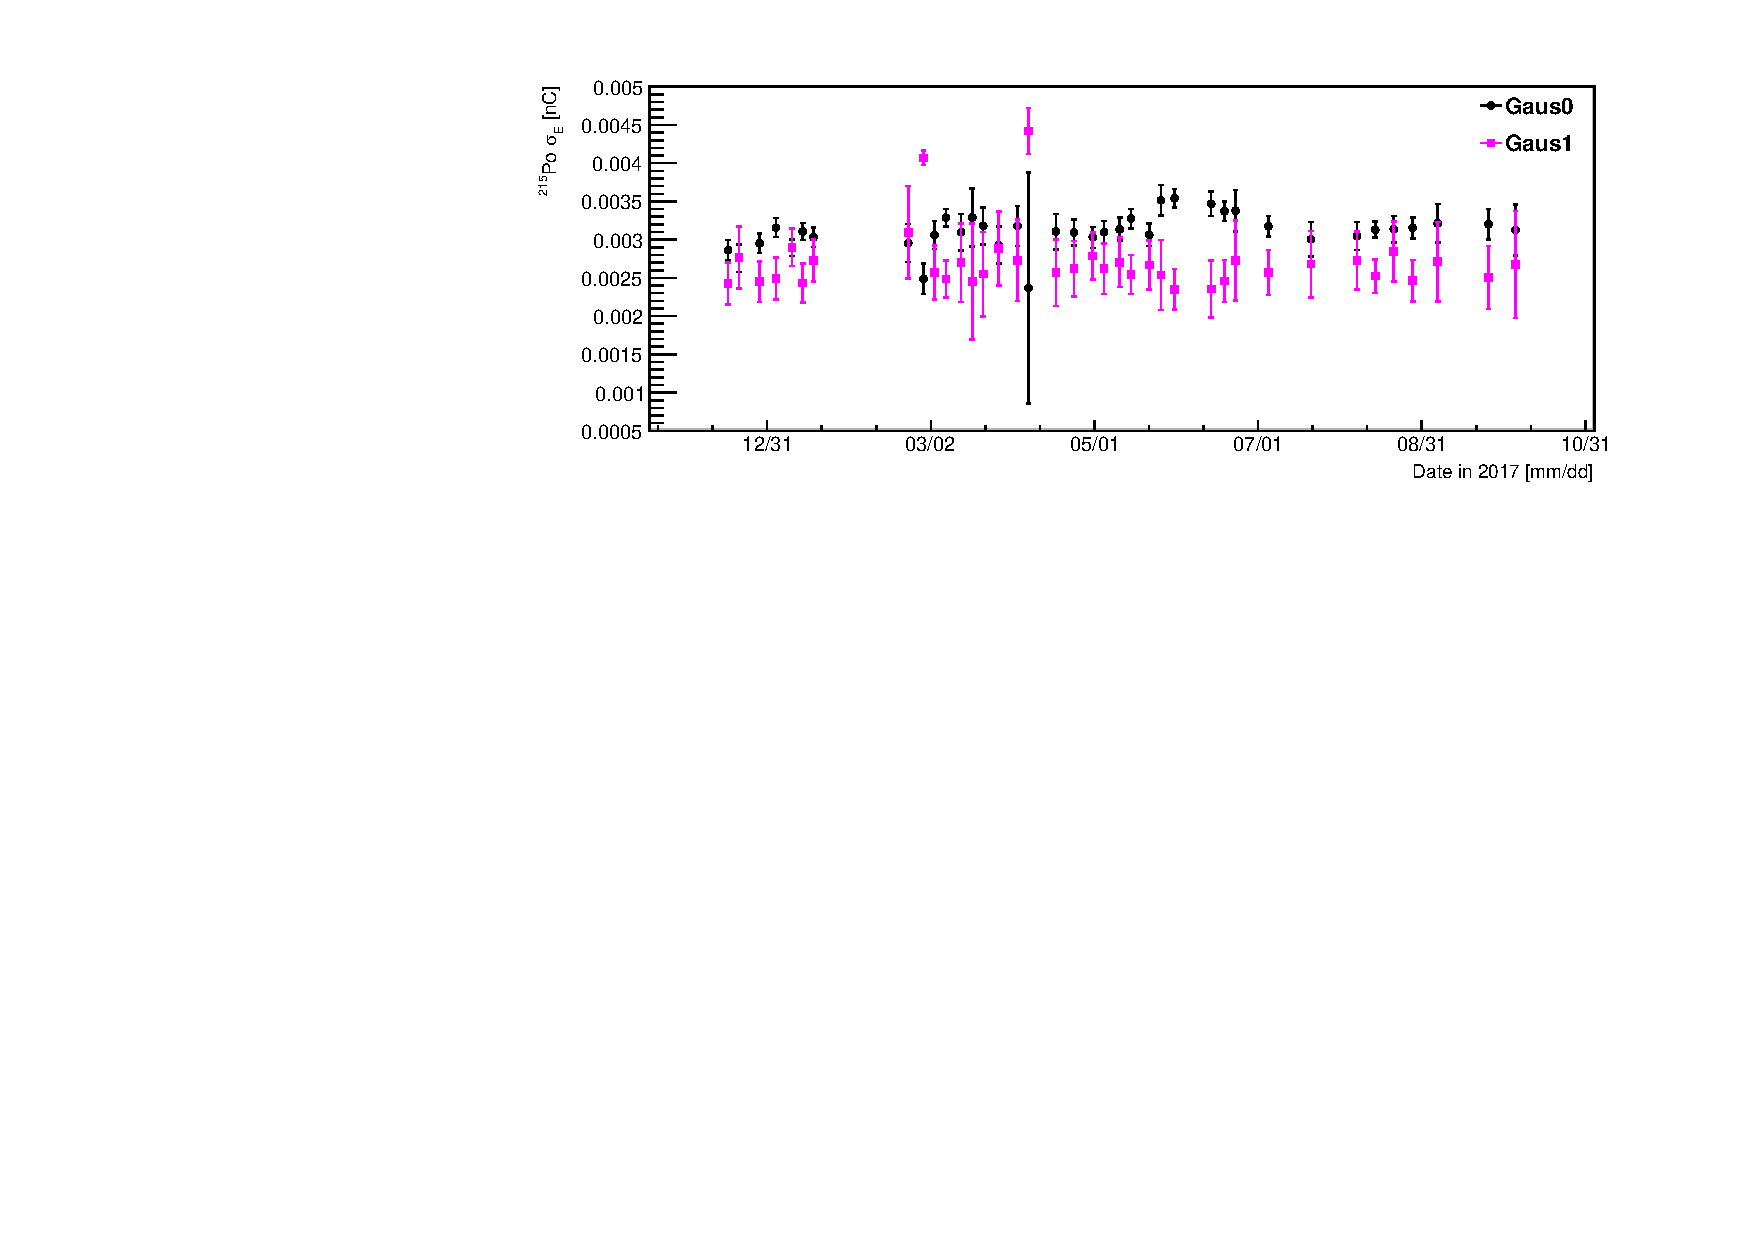
\includegraphics[width=0.9\linewidth]{tex/6-ac227-images/BNL/PoEnWidthVsTime_S2}
	\caption{The 1 $\sigma$ width of the two Gaussians fit to the \Po energy distributions for the reference sample.}
	\label{fig:poenwidthvstimes2}
\end{figure}

The amount of variation seen in measured rates and the \Po energy distribution indicate that the system was not repeatable and, as such, implies significant systematic errors that have not been accounted for. 
Though the PMT and acrylic holder were glued in place, the sample vials were repeatedly removed and replaced, possibly shifting the placement of the acrylic holder and the optical grease. 
This could possibly account for day-to-day variations, though large changes over time are not understood. 

To account for these variations all material sample rates, $R_M$, were compared to the reference sample rate, $R_{ref}$.
The ratio of the rates was calculated for each time bin as
\begin{equation}
ratio = \frac{R_M}{R_{ref.}}
\end{equation}
\begin{equation}
\sigma_{ratio} = ratio \times \sqrt{\left(\frac{\sigma_{M}}{R_{M}}\right)^2+\left(\frac{\sigma_{ref.}}{R_{ref.}}\right)^2}
\end{equation}
and the results are shown in Figure~\ref{fig:relratevstimeallsamples}.
The ratio of rates versus time, for each material, was fit with a constant and a straight line, the results of which are tabulated in Tables~\ref{tab:MatFitC} and \ref{tab:MatFitLine} respectively.

Except for the case of viton (discussed in the next section) there is no clear decrease in rate observed over the six month period for any material.
Though the chi-squared results for the constant fits are not ideal, the fits to a straight line result in slopes with 50\% error to greater than 100\% error, indicating that a decrease in rate is not a good model.
Variations in rate suggest large systematics that have not been accounted for, which imply that these results cannot be trusted to within $\sim \pm$10\%.
Though this may be true, the setup of the experiment, which included a large ratio of material surface area to LiLS area (greater than was true for the AD) and a much higher amount of \Ac activity than would be added to the PROSPECT AD, allowed for every chance of adsorption. 
As such, we could look for general trends that would indicate adsorption.
Since no obvious decreasing trends were observed and visual inspection of the vials determined that the scintillator had not degraded (yellowed) it was concluded that \Ac was not adsorbing onto materials and next steps were taken to include the source in the final detector.

\begin{figure}[H]
	\centering
	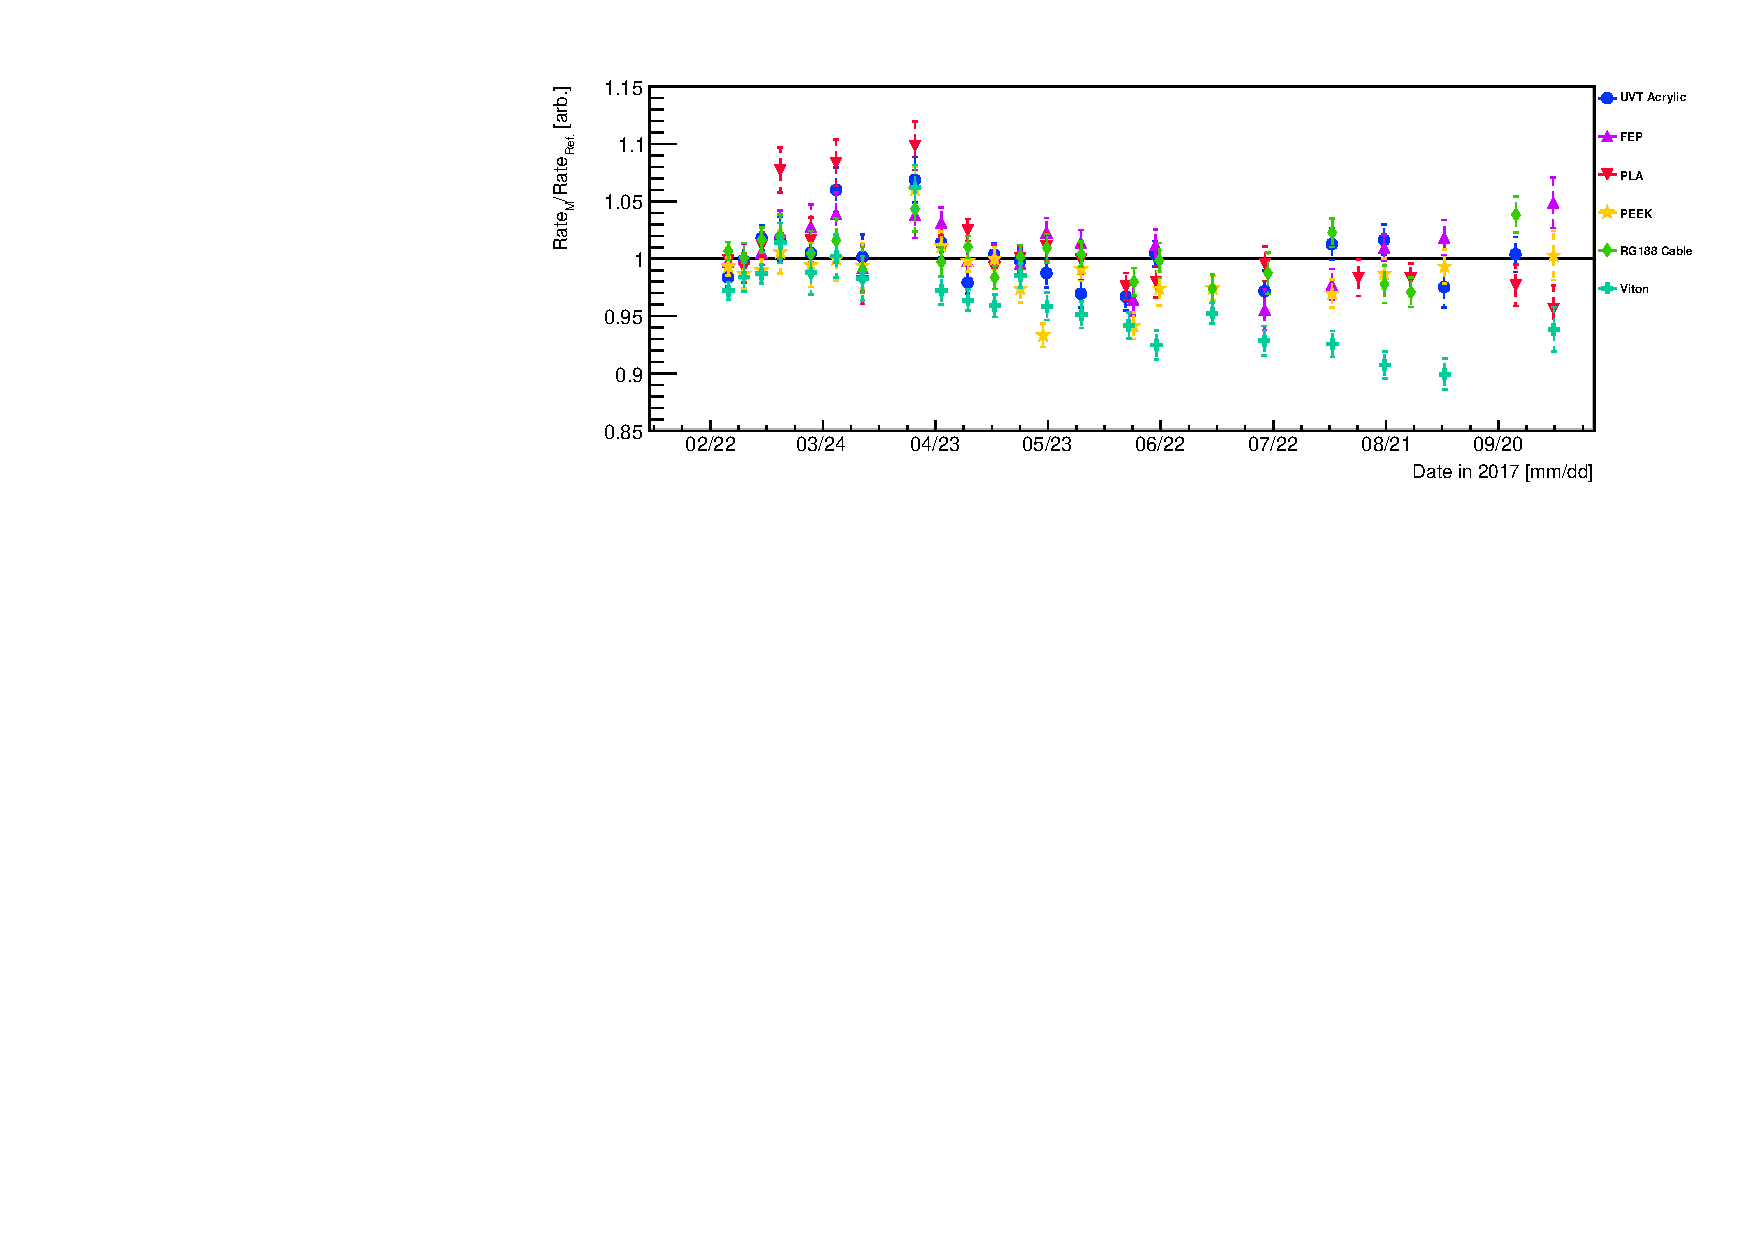
\includegraphics[width=1\linewidth]{tex/6-ac227-images/BNL/RelRateVsTime_AllSamples}
	\caption{\Ac rate for each material sample, $M$, relative to the reference sample.}
	\label{fig:relratevstimeallsamples}
\end{figure}

\begin{table}[H]
	\centering
\begin{tabular}{|c|c|c|}
	\hline 
	\textbf{Material} & \textbf{Constant} & \textbf{$\chi^2$/NDF} \\ 
	\hline 
	UVT Acrylic  & 0.997 $\pm$ 0.003 & 56.5/20 = 2.82 \\ 
	\hline 
	FEP & 1.005 $\pm$ 0.003 & 44.1/20 = 2.21 \\ 
	\hline 
	PLA & 1.003 $\pm$ 0.003 & 80.6/20 = 4.03 \\ 
	\hline 
	PEEK & 0.985 $\pm$ 0.003 & 70.9/20 = 3.55 \\ 
	\hline 
	RG188 Cable & 1.001 $\pm$ 0.003 & 38.3/21 = 1.82 \\ 
	\hline 
	Viton  & 0.960 $\pm$ 0.002 & 136.3/21 = 6.49 \\ 
	\hline 
\end{tabular} 
\caption{The results of fitting the relative rate for each material sample with a constant.}
\label{tab:MatFitC}
\end{table}

\begin{table}[H]
	\centering
\begin{tabular}{|c|c|c|c|}
	\hline 
	\textbf{Material} & \textbf{Constant} & \textbf{Slope [ratio/yr]} & \textbf{$\chi^2/NDF$} \\ 
	\hline 
	UVT Acrylic  & 1.5 $\pm$ 0.8 & -0.01 $\pm$ 0.02 & 56.2/19 = 2.96 \\ 
	\hline 
	FEP  & 1.3 $\pm$ 0.8 & -0.005 $\pm$ 0.018 & 44.0/19 = 2.32 \\ 
	\hline 
	PLA  & 4.4 $\pm$ 0.8 & -0.07 $\pm$ 0.02 & 64.3/19 = 3.38 \\ 
	\hline 
	PEEK  & 2.9 $\pm$ 0.8 & -0.04 $\pm$ 0.02 & 65.2/19 = 3.43 \\ 
	\hline 
	RG188 Cable  & 2.3 $\pm$ 0.8 & -0.03 $\pm$ 0.02 & 35.7/20 = 1.79\\ 
	\hline 
	Viton  & 7.7 $\pm$ 0.7 & -0.14 $\pm$ 0.02 & 48.9/20 = 2.45 \\ 
	\hline 
\end{tabular} 
\caption{The results of fitting the relative rate for each material with a straight line.}
\label{tab:MatFitLine}
\end{table}

\subsubsection{Viton}

Observation of the rate of \Ac in the viton o-ring material sample vial initially indicates a decrease in rate over time, about 10\% compared to the reference vial over a six month period.
Upon further inspection, though, it became clear that the energy spectrum, of the Rn events in particular, shift toward the system threshold as time goes on.
This caused a loss of events, not due to adsorbance, but rather due to threshold effects.

Figure~\ref{fig:rnpoenfirstandlast} shows the \Rn and \Po energy distributions in the first and last time bins for both viton and PEEK.
It can be seen that at the last time bin the viton distributions sit against the threshold, compared to the PEEK distributions which approach but do not get close to the threshold.
To quantify this the \Rn spectrum was fit with a sum of two Gaussians and the widths versus time are shown in Figure~\ref{fig:rnenwidths8}.
It can be seen that the lower energy Gaussian becomes narrower as time goes on, indicating a loss of events due to threshold effects.
Therefore, it was concluded that the decrease in \Ac rate observed in the viton o-ring sample was due to threshold effects rather than adsorption.


\begin{figure}[H]
	\begin{subfigure}{1\linewidth}
	\centering
	\includegraphics[width=1.\linewidth]{"tex/6-ac227-images/BNL/RnPoEn_FirstAndLast_S8"}
	%\caption{}
	\label{fig:rnpoenfirstandlasts8}
\end{subfigure}
\begin{subfigure}{1\linewidth}
	\centering
	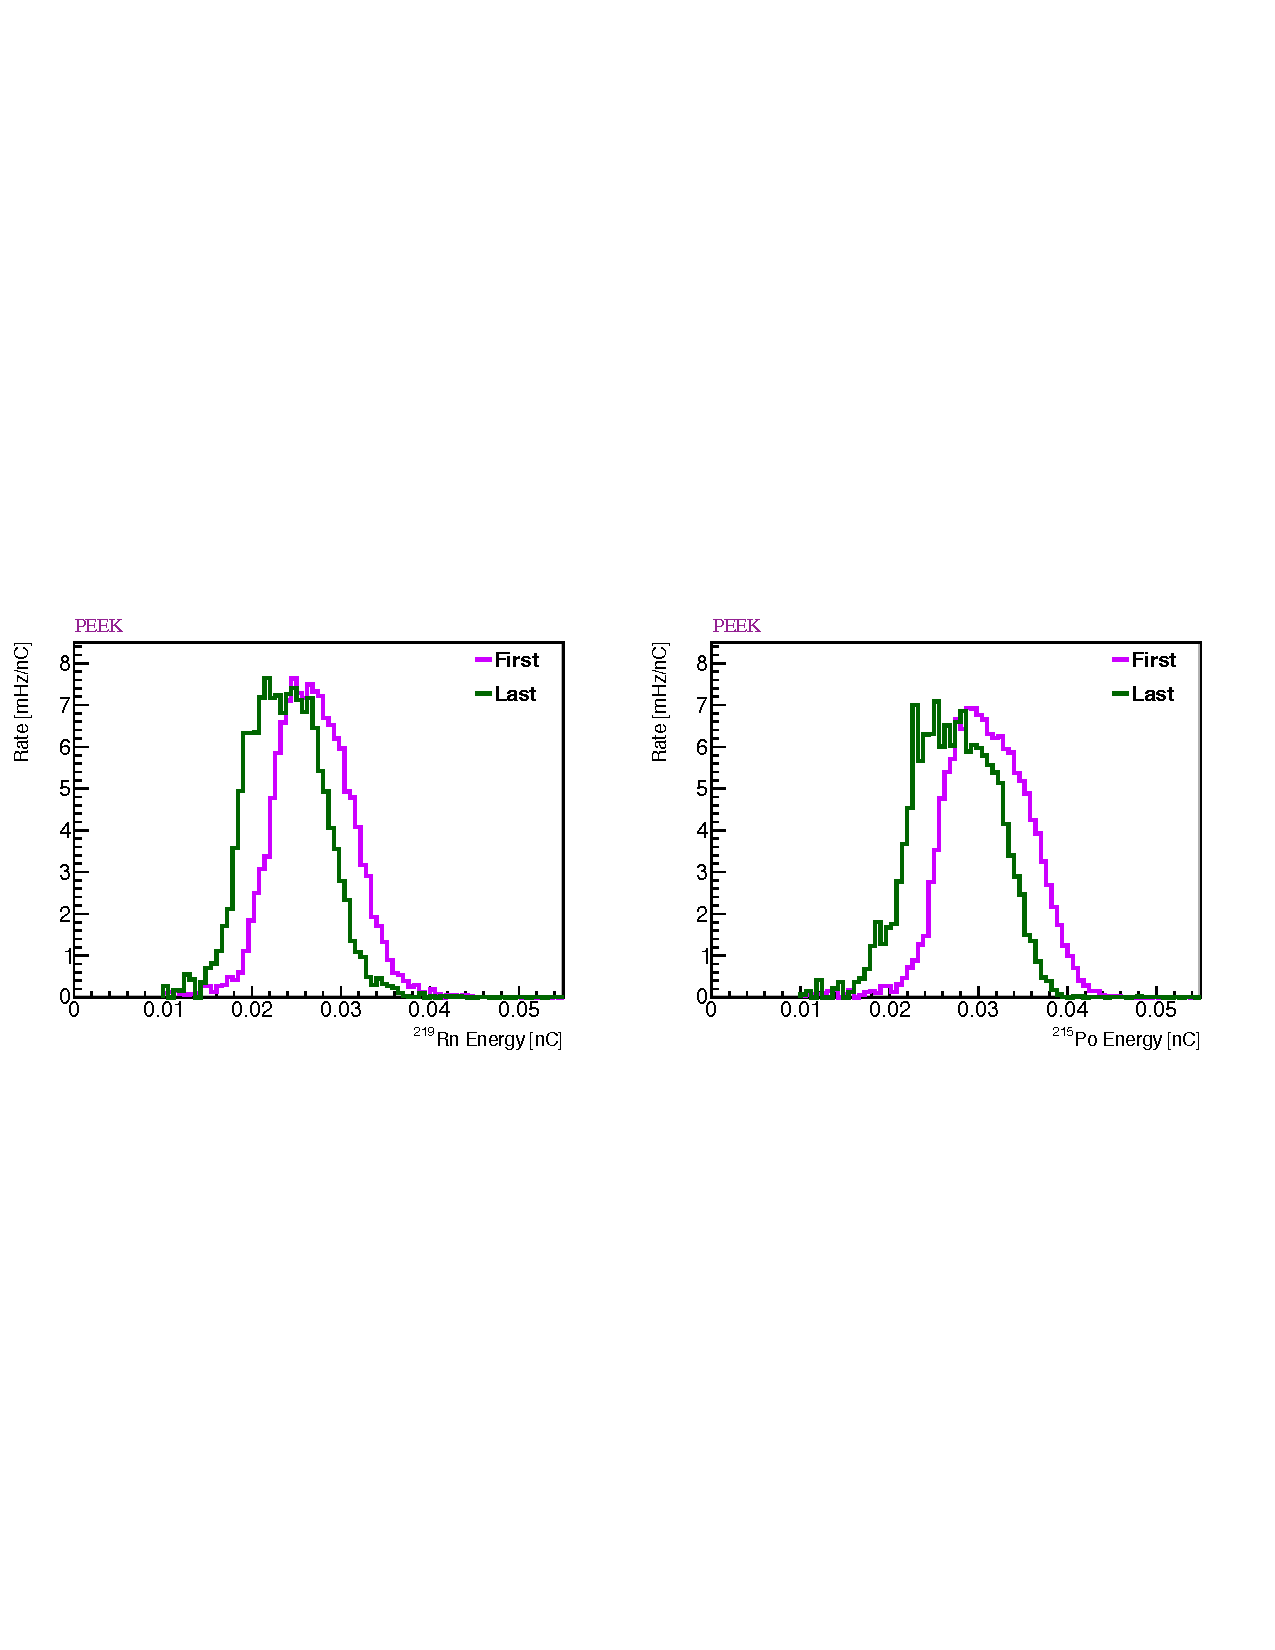
\includegraphics[width=1\linewidth]{tex/6-ac227-images/BNL/RnPoEn_FirstAndLast_S6}
	%\caption{}
	\label{fig:rnpoenfirstandlasts6}
\end{subfigure}
\caption{\Rn and \Po energy spectra for both the viton o-ring (top) and PEEK (bottom) material samples during the first and last time bins.}
\label{fig:rnpoenfirstandlast}
\end{figure}

\begin{figure}[H]
	\centering
	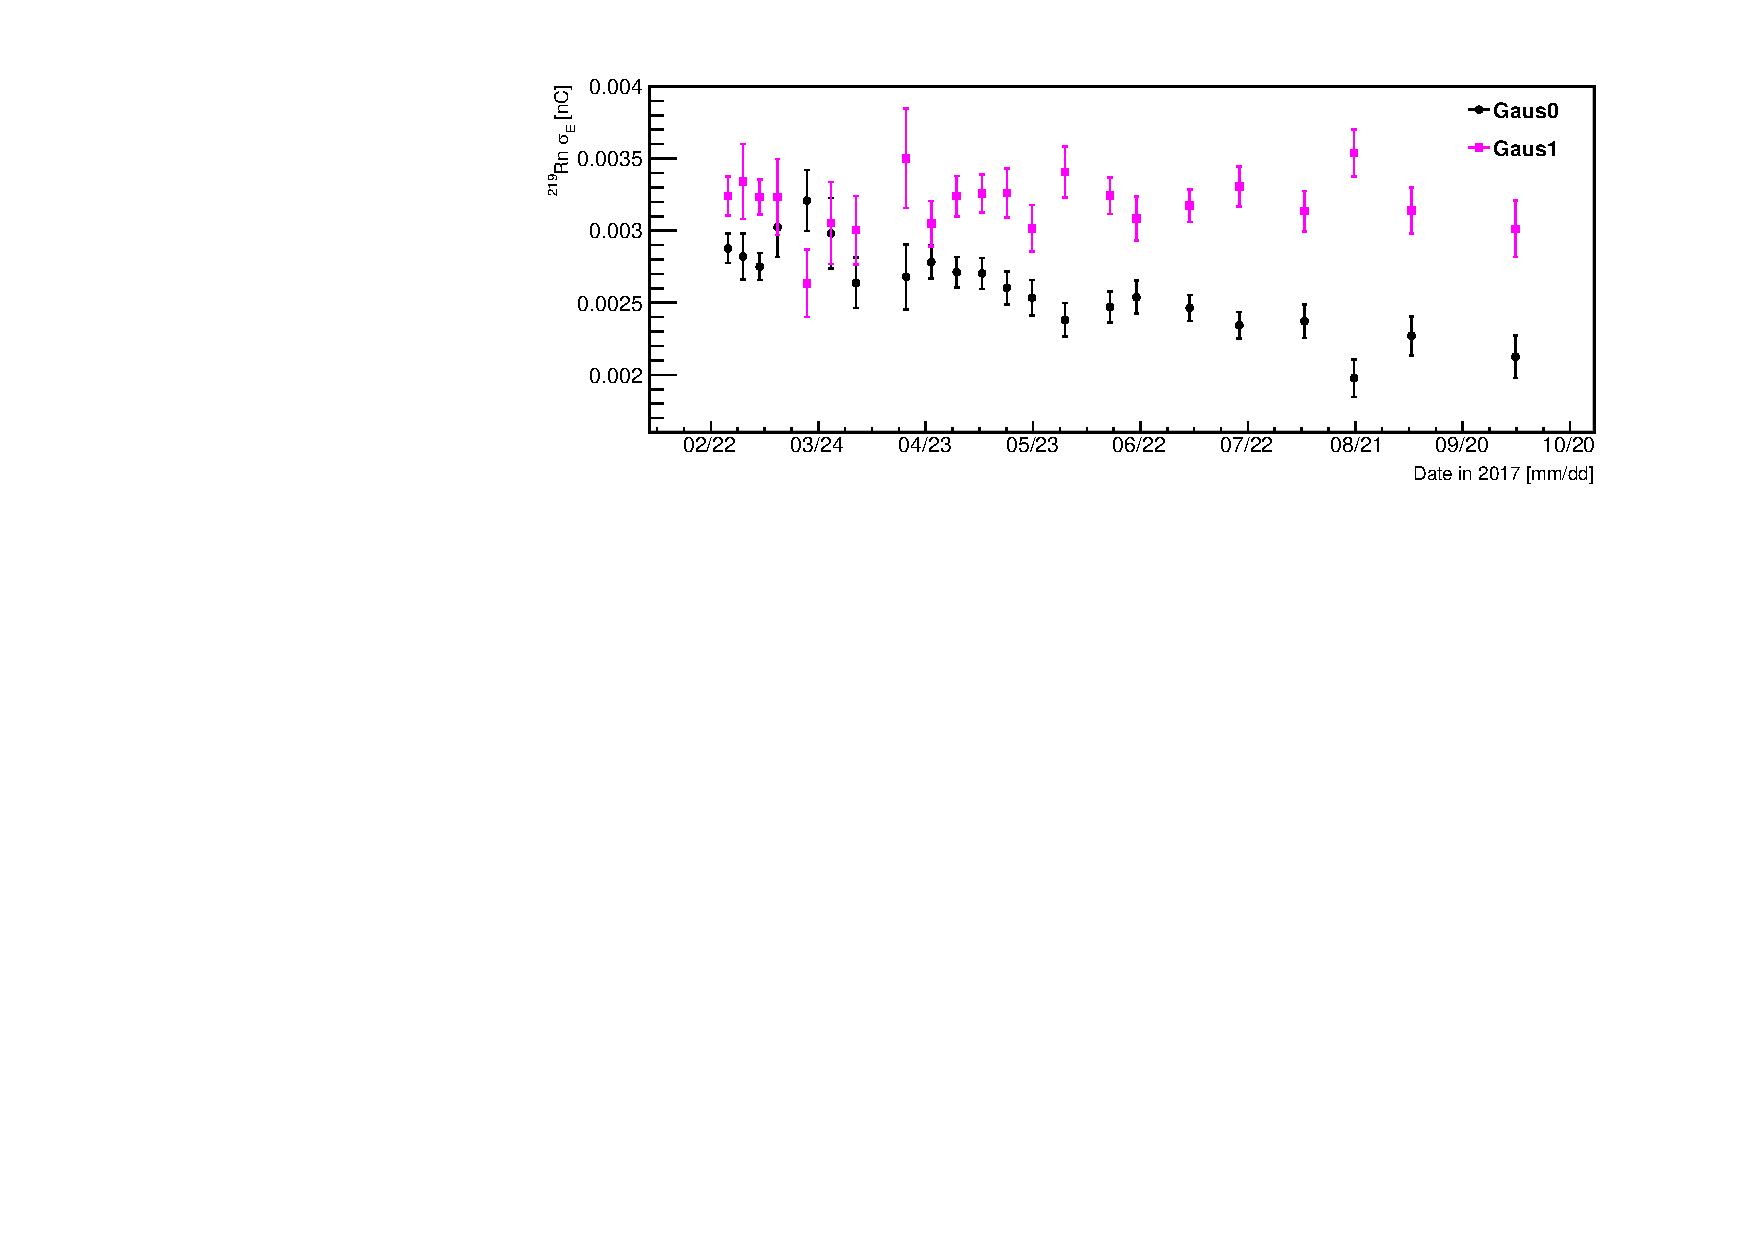
\includegraphics[width=0.9\linewidth]{tex/6-ac227-images/BNL/RnEnWidth_S8}
	\caption{The 1$\sigma$ width of two Gaussians fit to the \Rn energy spectrum versus time for the viton o-ring material sample. Black (circle): higher energy Gaussian, Magenta (square): lower energy Gaussian.}
	\label{fig:rnenwidths8}
\end{figure}



\section{\Ac in the PROSPECT AD}

Material compatibility testing determined that \Ac did not significantly adsorb onto detector materials, confirming that it could be used as a uniformly distributed source.
It will be noted here that \Ac spiked LiLS was added to a prototype detector that consisted of two stacked segments \cite{Ashenfelter:2018cli}.
This was done to determine that the \Ac did not degrade the performance of the liquid scintillator and that it did not introduce significant background.
Initial results from the prototype concluded that it did neither and provided the last step of evidence needed before addition to the full-scale detector.

\subsection{Spiking the LiLS}

After concluding that \Ac would be added to the AD, the goal was to obtain a final activity of 0.01 Bq/segment. 
Assuming a total LiLS mass of 4600 kg and an active mass of 3939 kg implies a total \Ac activity of 1.8 Bq.
The stock solution from which the LiLS was spiked was the same stock that was used for the material studies, which had an activity of $\sim$9.13 Bq/g on December 13, 2017, the day the spiking procedure was performed.
This means that $\sim$200 mg of the stock was needed to spike the LiLS.

In order to add \Ac to the total detector, a vial of spiked LiLS was added to a 55-gallon drum of LiLS prepared previously for detector filling.
Before the detector was filled all drums were added to an ISO-tank (a tank container which is built to the International Organization for Standardization standards) and bubbled with nitrogen to ensure thorough mixing of the LiLS from all drums and the \Ac.

We spiked the drum by diluting the concentration of the stock solution by adding it to an intermediate vial of production LiLS before spiking the vial that was added to the drum. 
This was done to reduce the relative uncertainty from the $\pm10$ mg uncertainty of the balance used to weigh the vials and allowed an assessment of the activity of the remaining vial.
The procedure was duplicated in a second set of vials so that the first vial could immediately be added to the LiLS drum and the second set could be used to measure the final activity and deduce that of the emptied one.

The spiking procedure was performed using four vials, V0, V1, V2, and V3.
The steps were:
\begin{enumerate}
	\item Fill all four vials with production LiLS
	\item Fill V1 and V2 with the \Ac spiked LiLS stock solution
	\item Fill V0 with solution from V1 until desired activity is reached
	\item Fill V3 with solution from V2 until desired activity is reached
	\item Empty V0 into drum of production LiLS 
\end{enumerate}
See Figure~\ref{fig:spikingprocedure} for a graphic of these steps along with Table~\ref{tab:SpikeProc} for a list of the weights of all solutions added and removed from the vials.
\begin{figure}[!b]
	\centering
	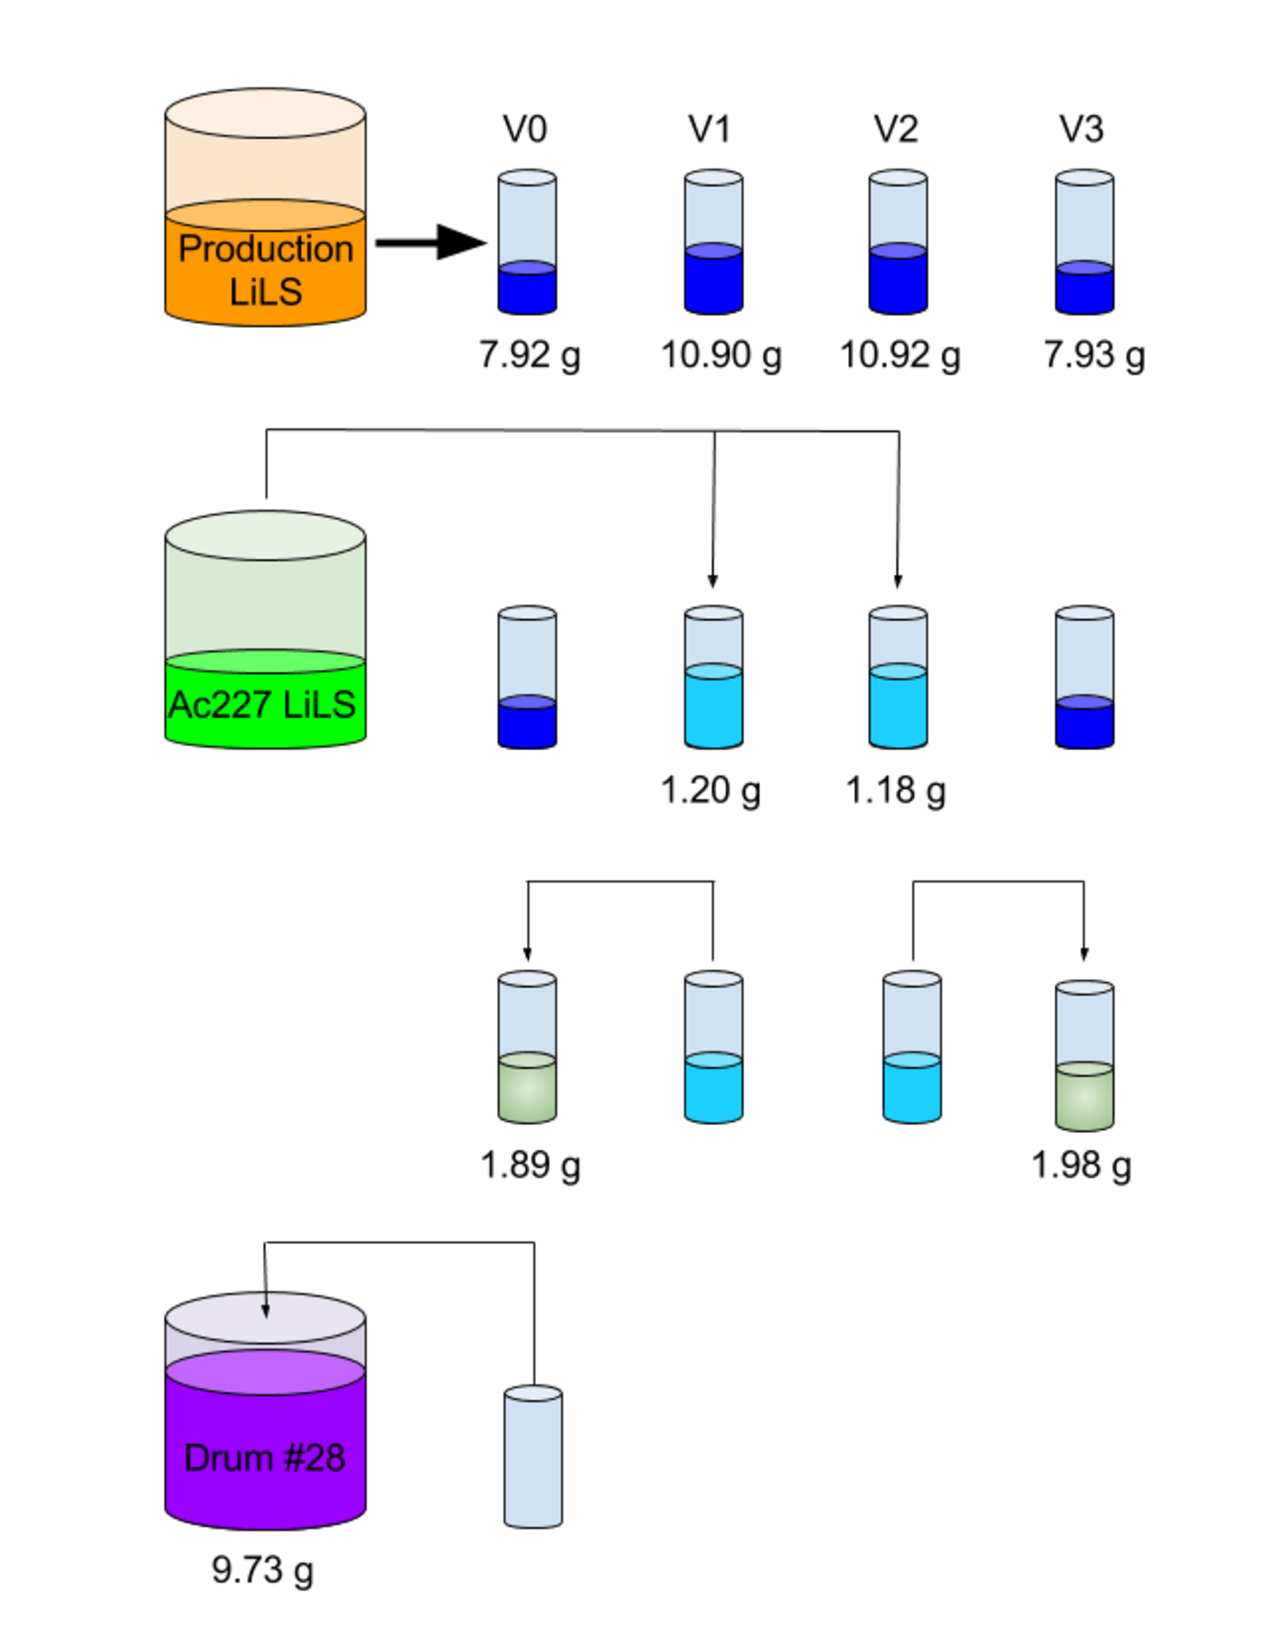
\includegraphics[width=0.5\linewidth]{tex/6-ac227-images/BNL/SpikingProcedure}
	\caption{A graphic of the procedure used to spike the drum of LiLS with \Ac for filling of the AD. The numbers indicate the amount of LiLS transfered, rather than the total weight.}
	\label{fig:spikingprocedure}
\end{figure}
The amount of LiLS that was transfered at each step was initially calculated so that $\sim$10 g would remain in all vials at the end.
The vials were filled and the transfers were completed using pipettes, therefore, some drops inevitably remained in the pipette at every step.
Vials V1 and V2 were gently swirled after the addition of the \Ac spiked LiLS in an attempt to mix the solution.

\begin{table}[!t]
	\centering
\begin{tabular}{r|c|c|c|c}
	\hline 
	& \textbf{V0} & \textbf{V1} & \textbf{V2} & \textbf{V3} \\ 
	\hline 
	\textbf{Production LiLS added, $m_1$ (g)}  & 7.92 & 10.90 & 10.92 & 7.925 \\ 
	\hline 
	\textbf{\Ac spiked solution added, $m_2$ (g)} &  & 1.20 & 1.18 &  \\ 
	\hline 
	\textbf{Solution removed, $m_3$ (g)} &  & 2.047 & 2.09 &  \\ 
	\hline 
	\textbf{Solution added, $m_4$ (g)} & 1.885 &  &  & 1.98 \\ 
	\hline 
\end{tabular} 
\caption{The weight of all solutions added and removed from the four vials for spiking of the LiLS with \Ac for filling of the AD.}
\label{tab:SpikeProc}
\end{table}

The expected \Ac rate, $A$, in vials V0(V3) was calculated as
\begin{equation}
	A = C~m_2 \frac{m_4}{m_1 + m_2}
\end{equation}
where $C$ is the activity of the \Ac spiked stock solution, 9.13 Bq/g, $m_1$ is the amount of production LiLS added to V1(V2), $m_2$ is the amount of the stock solution added to V1(V2), and $m_4$ is the amount of solution from V1(V2) that was added to V0(V3).
The expected rate in vials V1(V2) was then calculated as 
\begin{equation}
A = C~m_2 \left(1 - \frac{m_3}{m_1 + m_2}\right)
\end{equation}
where $m_3$ is the amount of solution removed from V1(V2).
The expected \Ac activity for each vial is listed in Table~\ref{tab:SpikeExpA}.

The \Ac rate in vials V1, V2, and V3 were measured after adding V0 to the drum of LiLS.
The rate of \Ac in V3 should be similar to the rate in AD, recalling that the goal was 1.8 Bq.
A plot of the measured rates for each vial is shown in Figure~\ref{fig:ADVials}.
Each of these rates was fit with a constant, with the results of these fits listed in Table~\ref{tab:SpikeExpA}.
\begin{table}[h]
	\centering
	\begin{tabular}{c|c|c}
		\hline 
		\textbf{Vial} & \textbf{Expected Activity [Bq]} & \textbf{Measured Rate [Hz]} \\ 
		\hline 
		V0 & 1.71 & \\ 
		\hline 
		V1 & 9.10 &  9.48 $\pm$ 0.04  \\ 
		\hline 
		V2 & 8.91 & 9.38 $\pm$ 0.06\\ 
		\hline 
		V3 & 1.76 & 0.696 $\pm$ 0.001 \\ 
		\hline 
	\end{tabular} 
	\caption{Expected and measured \Ac activity in vials prepared for spiking the LiLS. }
	\label{tab:SpikeExpA}
\end{table}
It can be seen that the measured rates in V1 and V2 are about 4\% higher than expectation, and the rate in V3 is about 50\% lower.
A possible explanation for this discrepancy is that the solution was not sufficiently mixed before transferring between the stock solution and the vials and between the vials themselves. 
This is bolstered by the fact that the measured rates in V2+V3 = 10.08 Hz, compared to the expected rate of 10.67 Hz, well within a 10\% systematic error that could be assigned from uncertainties in the mixing and measurement procedure.

If this experiment was repeated a more thorough testing of transfer procedures would need to be performed.
In conclusion, the measured rate in V3 indicates that the \Ac rate in the PROSPECT AD should be around 0.7 Hz in the total volume ($\sim$0.6 Hz in the active volume), less than half of the initial goal.

\begin{figure}[!t]
	\centering
\begin{subfigure}{1\linewidth}
	\centering
	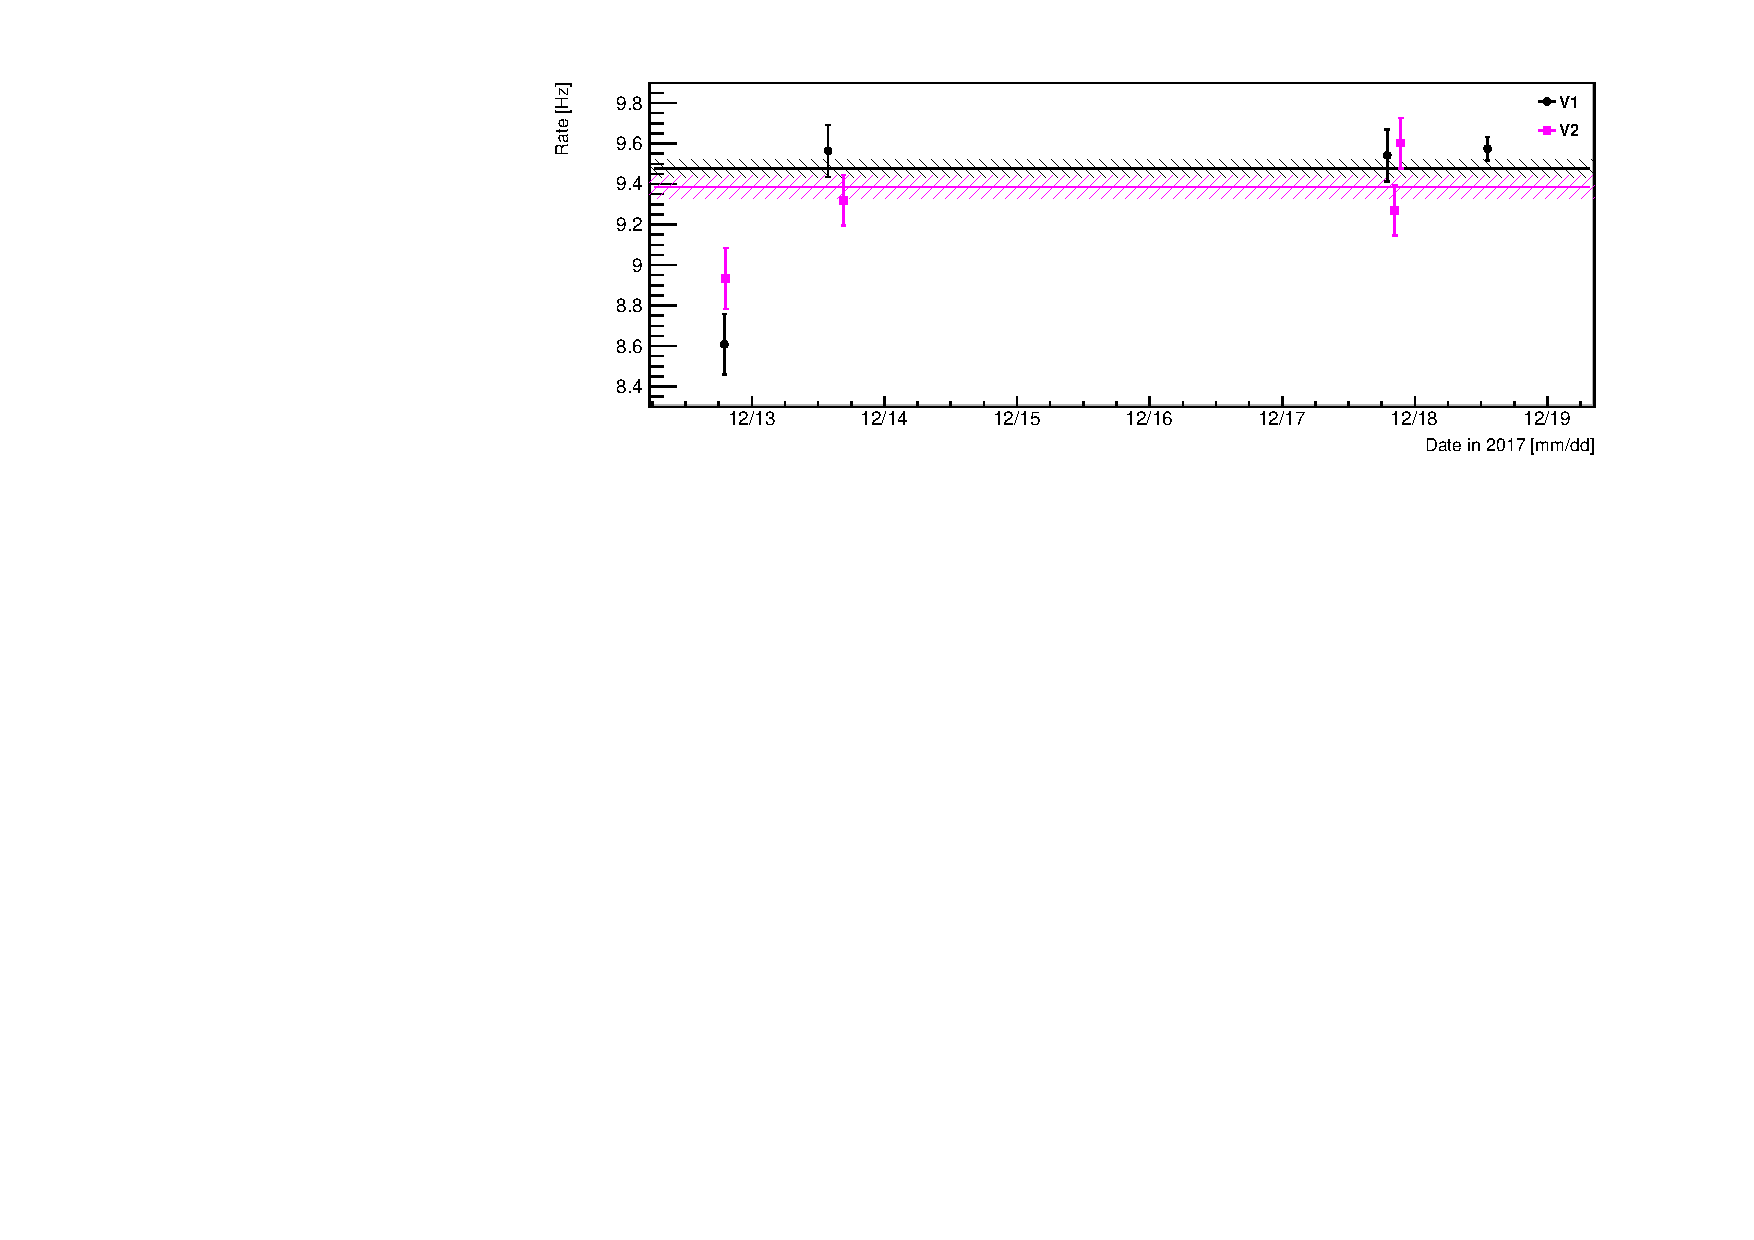
\includegraphics[width=0.9\linewidth]{tex/6-ac227-images/BNL/AD_Rates}
	%\caption{}
	\label{fig:adrates}
\end{subfigure}
\begin{subfigure}{1\linewidth}
	\centering
	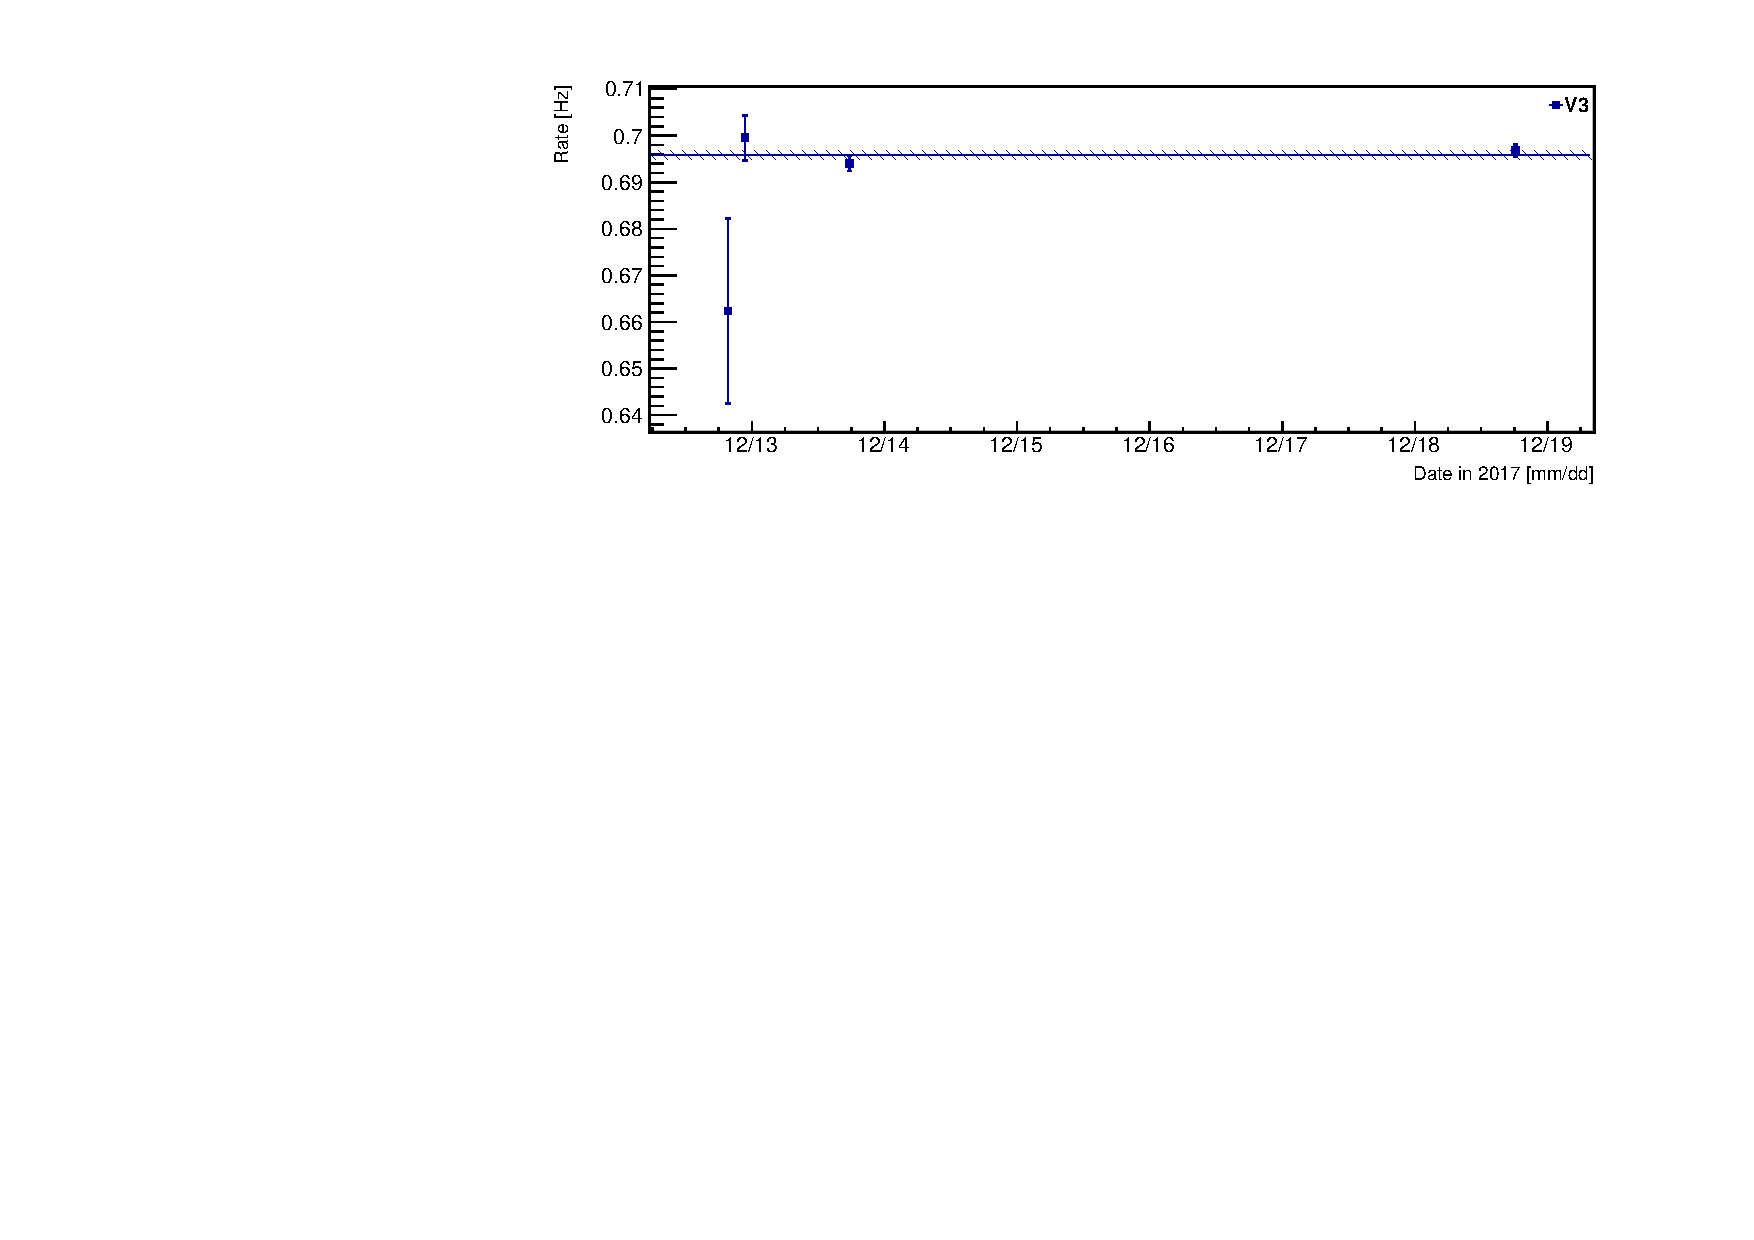
\includegraphics[width=0.9\linewidth]{tex/6-ac227-images/BNL/AD_RateV3}
	%\caption{}
	\label{fig:adratev3}
\end{subfigure}
\caption{Measured \Ac rates of vials used in the procedure performed to add \Ac to the LiLS of the PROSPECT AD. Top: intermediate vials V1 and V2. Bottom: V3, filled in the same method as the vial that was added to the drum of LiLS. All rates were fit with a constant, the results drawn as solid lines with hashed lines representing the error.}
\label{fig:ADVials}
\end{figure}


\subsection{Data Set}

PROSPECT began taking data in March 2018.
The data set used for the \Ac analysis ran from March 5, 2018 - October 6, 2018, with a break from March 31, 2018 - April 17, 2018 when the detector was off for maintenance. 
The total runtime was 4048.9 hrs (2293.7 hrs reactor on, 1755.2 hrs reactor off), with 4011.7 hrs of livetime data.

During the data collection period used for this analysis, several PMTs exhibited abnormal behavior, including current instabilities, and are no longer in operation.
Preliminary theories for the cause of this are that LiLS leaked into the PMT housings and damaged the voltage dividers, but this has yet to be confirmed. 
To account for this all segments that `turned off' during the data period are excluded in this analysis. 
The result is 90 active segments, as shown in Figure~\ref{fig:segments}.

\begin{figure}[h]
	\centering
	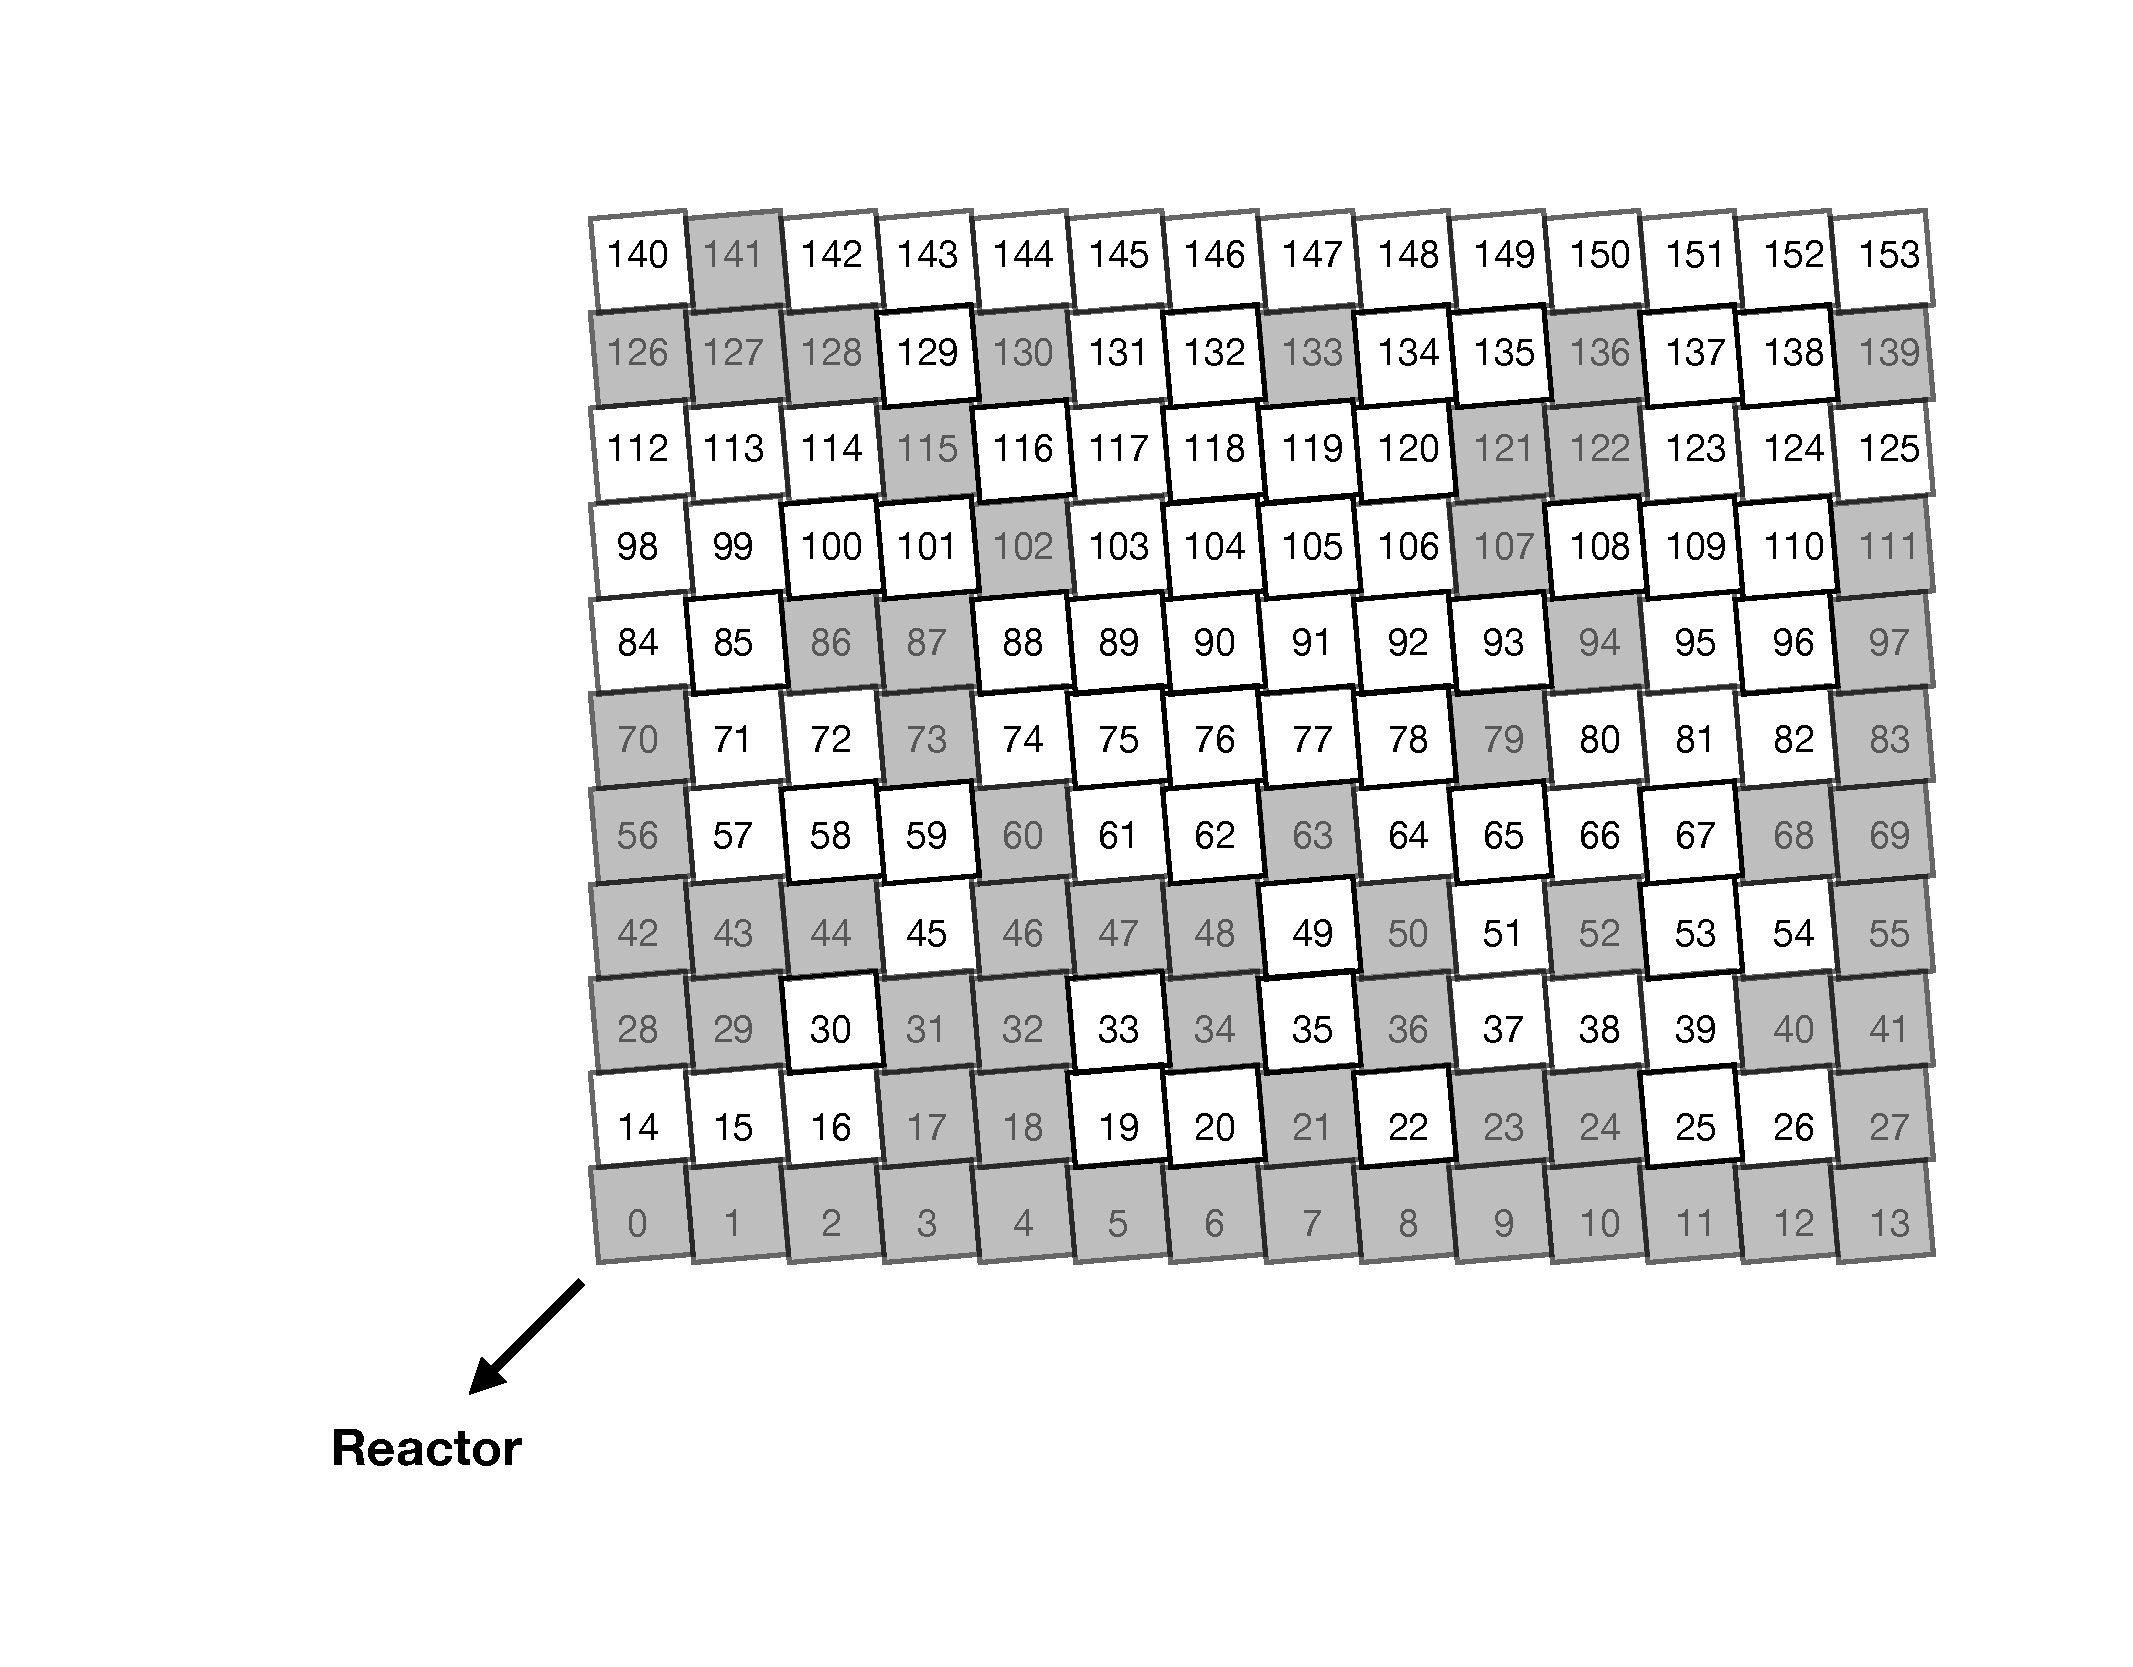
\includegraphics[width=0.7\linewidth]{tex/6-ac227-images/AD_DataSet/Segments}
	\caption{Graphic of 154 segments of the PROSPECT AD. Grayed out segments are those that `turned off' during the data period and are excluded in this analysis.}
	\label{fig:segments}
\end{figure}


\subsection{Event Selection}

RnPo events in the PROSPECT detector were found by looking at event clusters.
A cluster is defined as a collection of events that occur within 20 ns of each other.
Time coincident events were found by first looking for delayed (Po) events. 
These events were required to be in a single multiplicity cluster, because \Po emits a single mono-energetic alpha with no accompanying gammas, and pass broad energy and PSD cuts as outlined in Table~\ref{tab:RnPoCuts}.

We identified coincident prompt events by looking in a 5$\tau$ time window before the delay event, where $\tau = 2.57$ ms is the lifetime of $^{215}$Po.
We required that the highest energy event in a given cluster in that time window occurred in the same segment as the delay event and passed the energy and PSD cuts in Table~\ref{tab:RnPoCuts}.
Due to the close proximity to the neutron capture on $^6$Li signal ($\sim$0.55 MeV), only events where $\Delta t = t_{\textrm{delay}}-t_{\textrm{prompt}} > 0.5$~ms were accepted.
Since the neutron capture time in PROSPECT is about 50 $\mu$s, this cut effectively removes any chance of neutron contamination in the event selection.
The prompt and delayed alphas are expected to be within a few tens of microns of each other, but, due to detector position resolution, $\Delta z = \abs{z_{\textrm{delay}} - z_{\textrm{prompt}}}$ was required to be less than 250~mm.

Accidental prompt events were found by looking in a 5$\tau$ time window offset 10$\tau$ before the delay event. 
The same cuts applied to coincidental prompt events were applied to accidental prompt events.

\begin{table}[!t]
	\centering
\begin{tabular}{c|c}
	\hline 
	Prompt Energy & 0.48 $<$ E $<$ 1.18 MeV \\ 
	\hline 
	Delay Energy & 0.61 $<$ E $<$ 1.18 MeV \\ 
	\hline 
	PSD & 0.16 $<$ PSD $<$ 0.36 \\ 
	\hline 
	$\Delta z = |z_{\textrm{delay}} - z_{\textrm{prompt}}|$ & $\Delta z < 250$ mm  \\ 
	\hline 
	$\Delta t = t_{\textrm{delay}} - t_{\textrm{prompt}}$ & $0.5 < \Delta t < 5\tau$ ms \\ 
	\hline 
\end{tabular} 
\caption{First pass, broad cuts used to find RnPo events, where $\tau = 2.57~\textrm{ms}$ is the lifetime of \Po. A second pass of the data changes the requirement for the low bounds of energy and PSD to be $< 4 \sigma$ from the mean.}
\label{tab:RnPoCuts}
\end{table}

In addition to energy, PSD, and position cuts a pileup veto was applied to all events.
At the time of a trigger event all boards are signaled to begin a 592 ns acquisition window. 
Events arriving at the end of this window do not re-trigger the data acquisition system, thus causing truncated waveforms.
In order to avoid using these truncated events, any cluster preceded by another cluster in a 800 ns window is vetoed. 

The broad energy and PSD cuts listed in Table~\ref{tab:RnPoCuts} are applied on a first pass analysis of the PROSPECT data.
Changes in detector performance over time, including decreasing energy resolution and PSD, required a second pass of the data, in which the lower bounds of the energy and PSD cuts were changed to be 4$\sigma$ lower than the mean of the distributions for a given time bin or segment.
The range of 4$\sigma$ was chosen in order to avoid large efficiency corrections for these cuts.

To check if these cuts correctly selected RnPo events, one can look at the position distribution of \Po events along $z$, as shown for one segment in Figure~\ref{fig:poposseg76}.
As expected this distribution is fairly stable across the length of the segment and almost all events are reconstructed inside of the physical length of the cell (a small percentage are reconstructed in the mineral oil in the front of the PMT face).
The PSD versus energy and \Po energy versus \Rn energy distributions, after accidental subtraction, can be seen in Figure~\ref{fig:RnPoPSDEn}.

\begin{figure}[h]
	\centering
	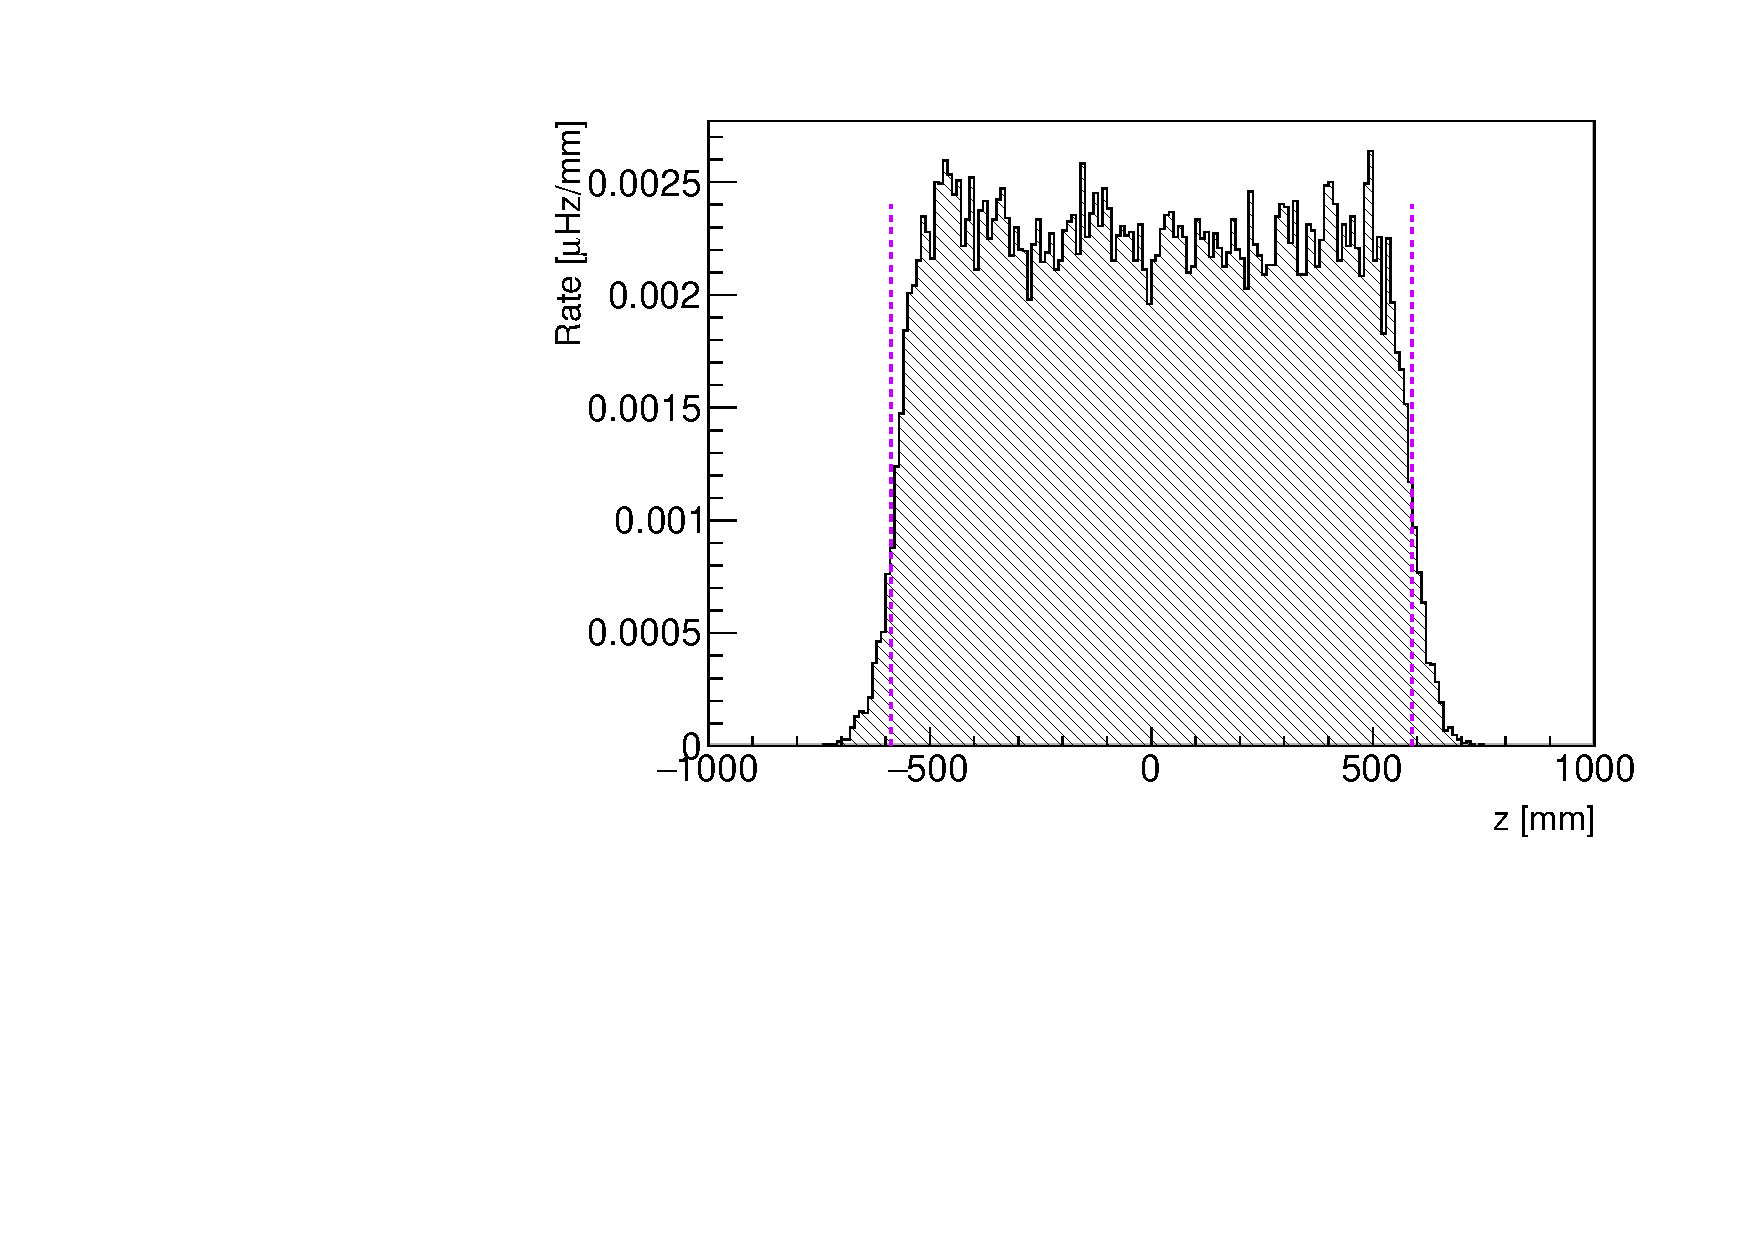
\includegraphics[width=0.6\linewidth]{tex/6-ac227-images/AD_EventSelection/PoPos_Seg76}
	\caption{Reconstructed position distribution for \Po events in a typical segment integrated over all time. Vertical dashed lines (purple) are drawn at the limits of the physical length of the segment.}
	\label{fig:poposseg76}
\end{figure}

\begin{figure}[h]
	\centering
	\begin{subfigure}{0.5\linewidth}
		\centering
		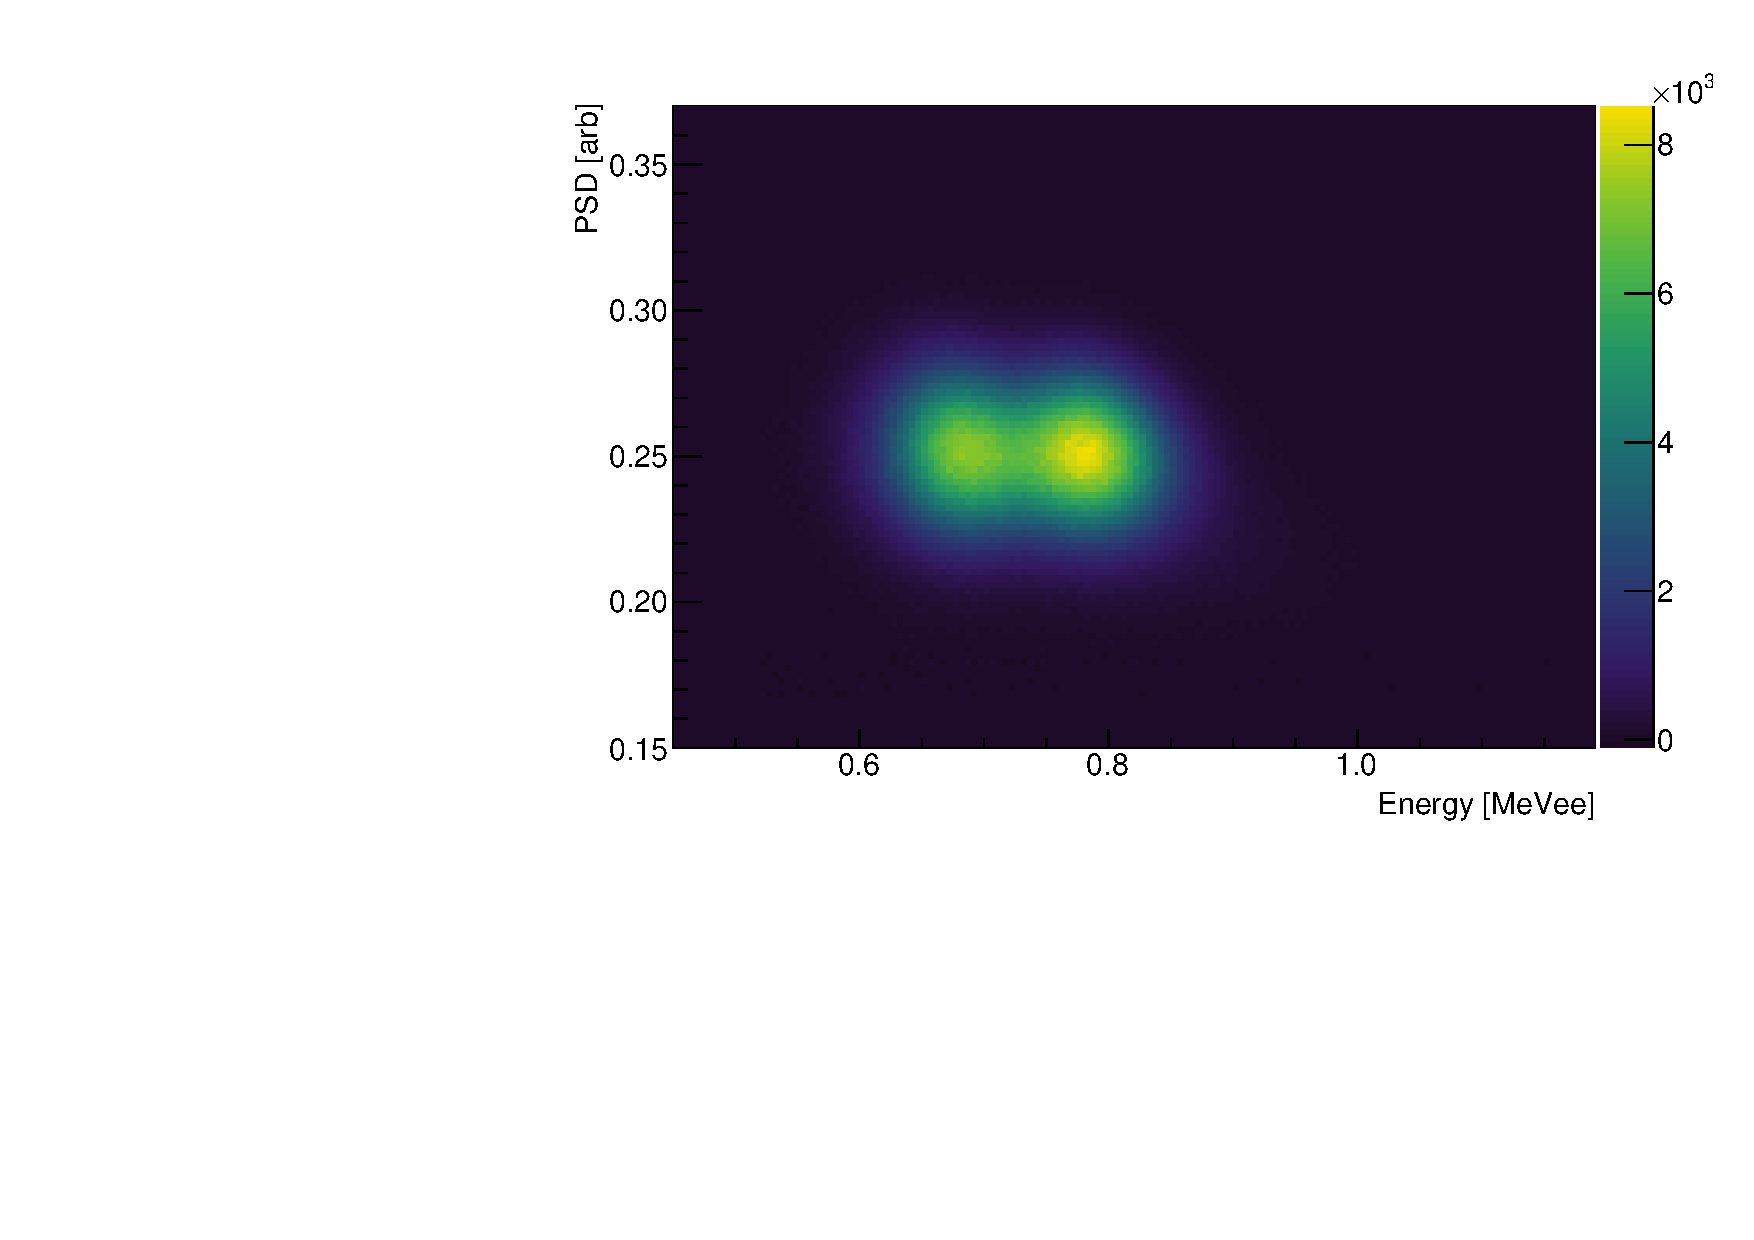
\includegraphics[width=0.9\linewidth]{tex/6-ac227-images/AD_EventSelection/RnPoPSDvsEn_AllCellsAllTime_Time0}
		\caption{RnPo PSD versus Energy.}
		\label{fig:rnpopsdvsentimebin0}
	\end{subfigure}\hspace{0cm}%
	\begin{subfigure}{0.5\linewidth}
		\centering
		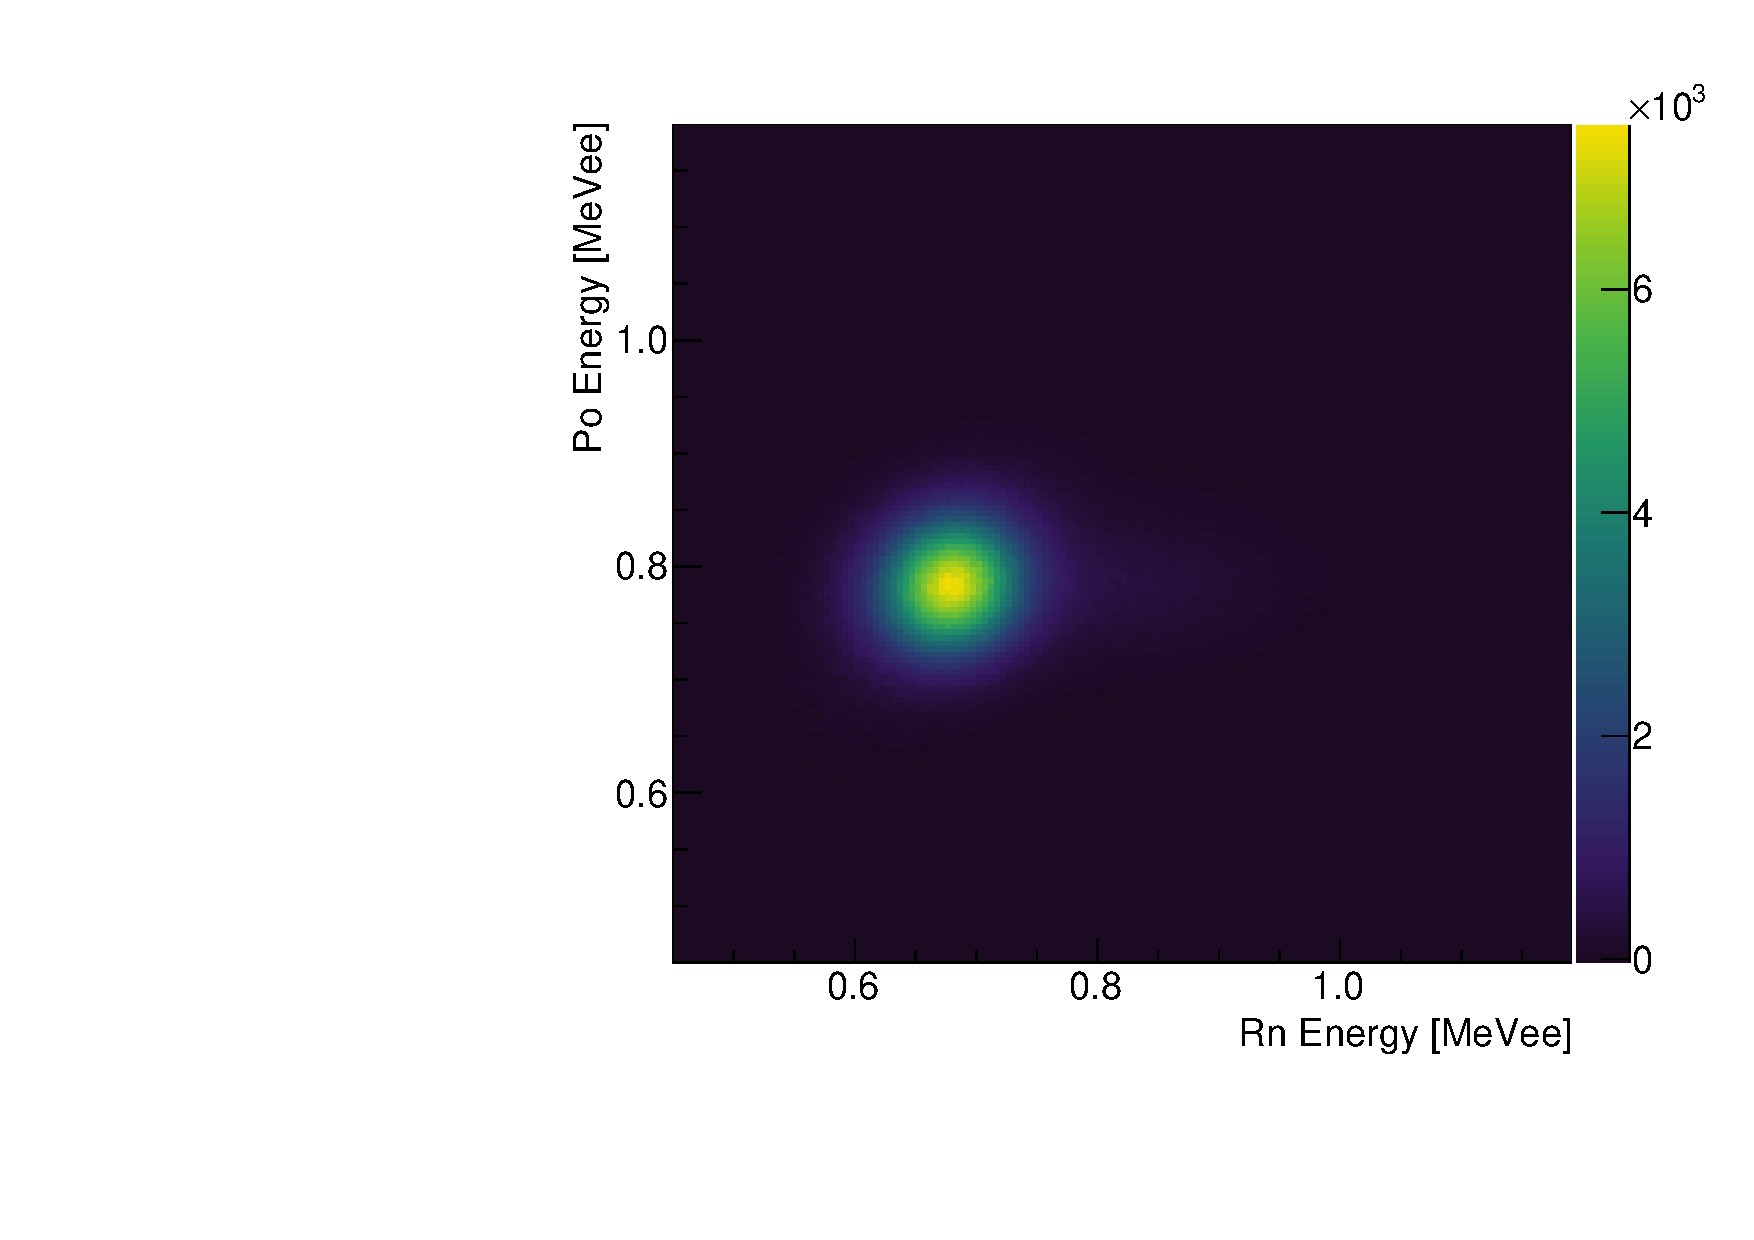
\includegraphics[width=0.7\linewidth]{tex/6-ac227-images/AD_EventSelection/PoEnvsRnEn_AllCellsAllTime_Time0}
		\caption{\Po energy versus \Rn energy.}
		\label{fig:poenvsrnentimebin0}
	\end{subfigure}
	\caption{RnPo distributions for all cells integrated over all time.}
	\label{fig:RnPoPSDEn}
\end{figure}



\subsection{Rate Calculation}

The \Ac rate per segment, or for a given time period, was found by fitting the background subtracted $\Delta t$ distribution, where $\Delta t = t_{\textrm{delay}} - t_{\textrm{prompt}}$, with
\begin{equation}
	f(t) = Ne^{-t/\tau}
	\label{eq:dtexp}
\end{equation}
where $N$ and $\tau$, the lifetime of $^{215}$Po, were allowed to vary.
For an example of these distributions and fit for a typical segment see Figure~\ref{fig:rnpodtseg76}.
The rate was then calculated as
\begin{equation}
	R = \frac{N~\tau}{\Delta t\textrm{-bin-width}\times\textrm{livetime}\times\textrm{efficiency}}
\end{equation}
\begin{equation}
	\sigma_R = R \times \sqrt{\left(\frac{\sigma_N}{N}\right)^2 + \left(\frac{\sigma_\tau}{\tau}\right)^2  +  \frac{2\sigma_{N\tau}}{N\tau} + \left(\frac{\sigma_{eff.}}{eff.}\right)^2}
\end{equation}
where $N$ and $\tau$ are results of the $\Delta t$ fit.
The robustness of this fit can be tracked by observing the resulting values for $\tau$ per individual segment and versus time for all segments and comparing the averages to the currently accepted value for the lifetime of $^{215}$Po, 2.569 $\pm$ 0.007 ms.
These results are shown in Figure~\ref{fig:tau}.
The average lifetime per individual segment is 2.564 $\pm$ 0.002ms, and versus time for all segments in 2.565 $\pm$ 0.002 ms, in great agreement with the accepted lifetime.

\begin{figure}[h]
	\centering
	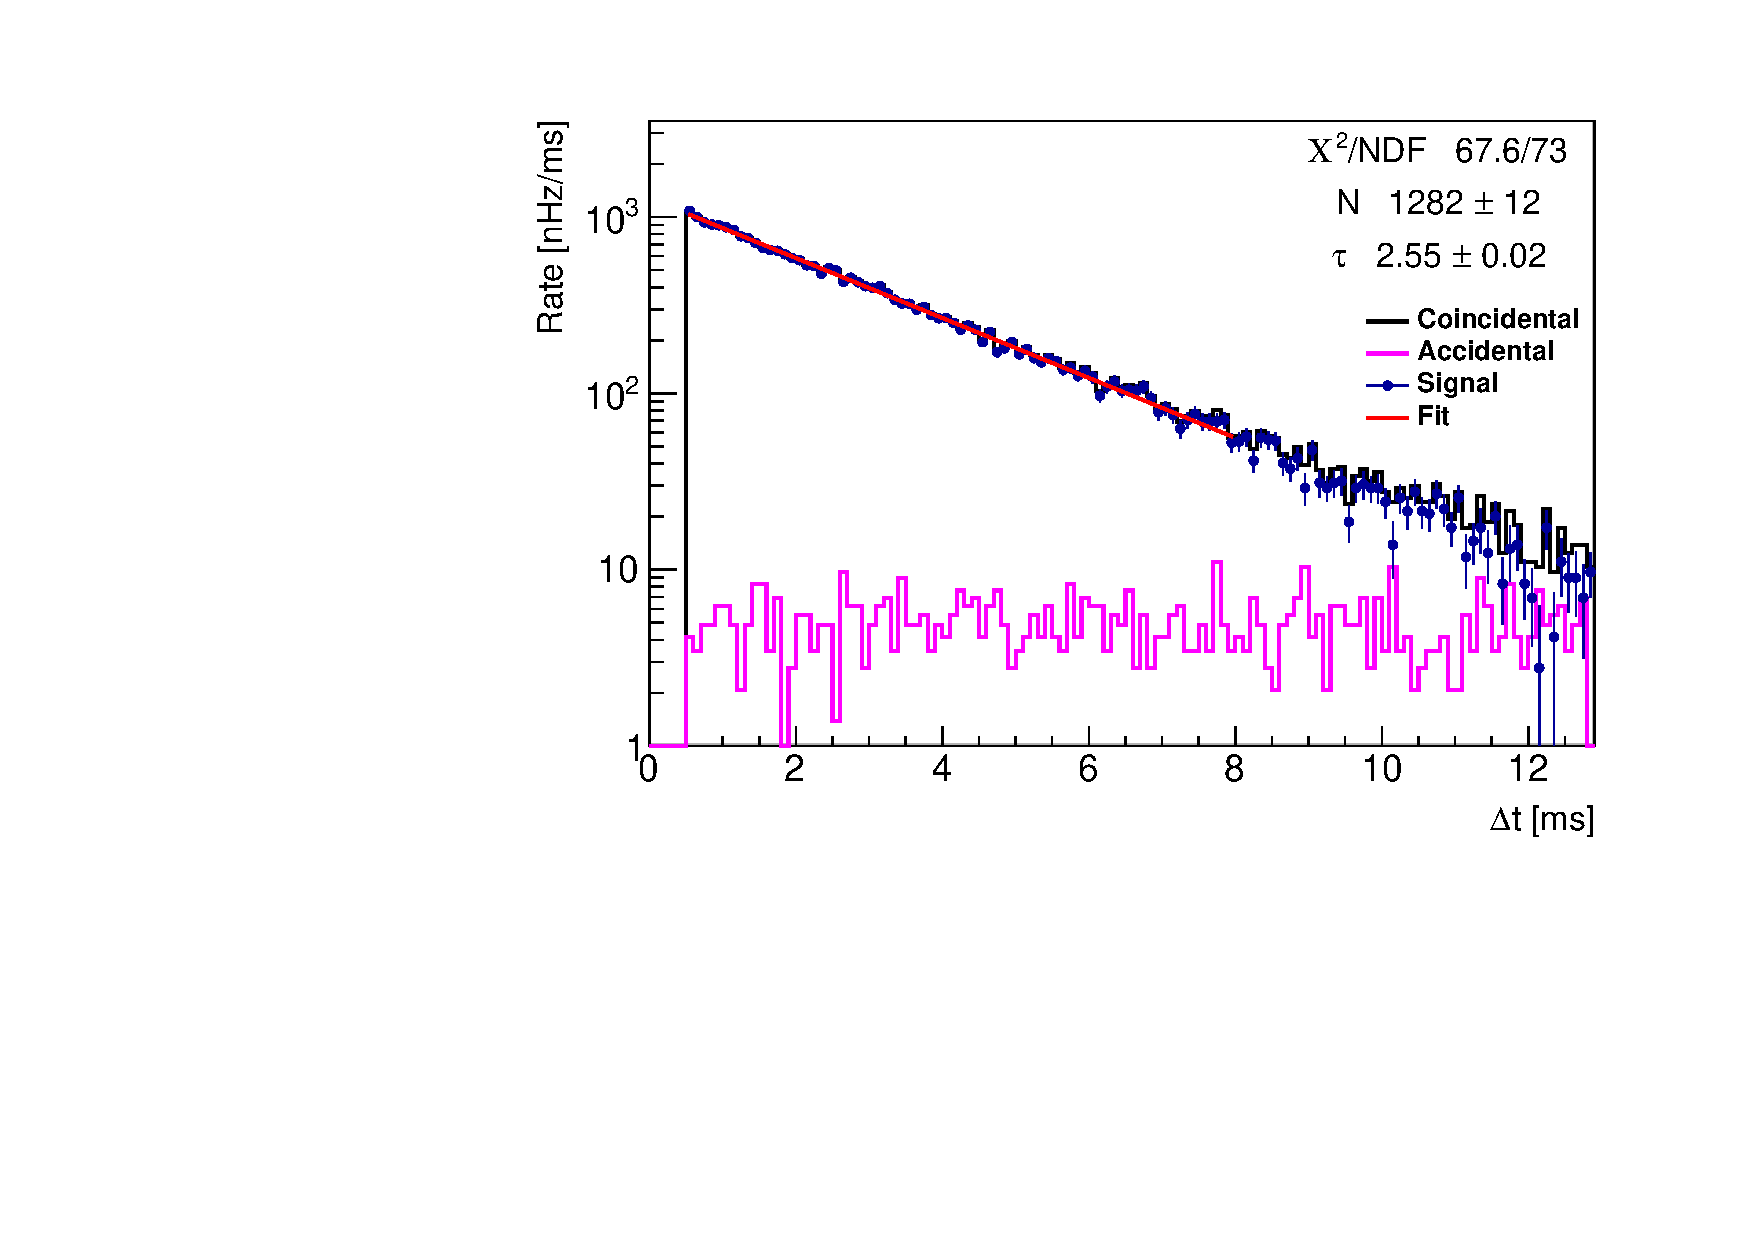
\includegraphics[width=0.65\linewidth]{tex/6-ac227-images/AD_RateCalc/RnPoDt_Seg76}
	\caption{Coincidental (black), accidental (magenta), and background subtracted (blue) $\Delta t$ distributions for a typical segment integrated over all time. A fit of Equation~\ref{eq:dtexp} to the background subtraction distribution is shown in red along with its results.}
	\label{fig:rnpodtseg76}
\end{figure}

\begin{figure}[h]
	\begin{subfigure}{1\linewidth}
	\centering
	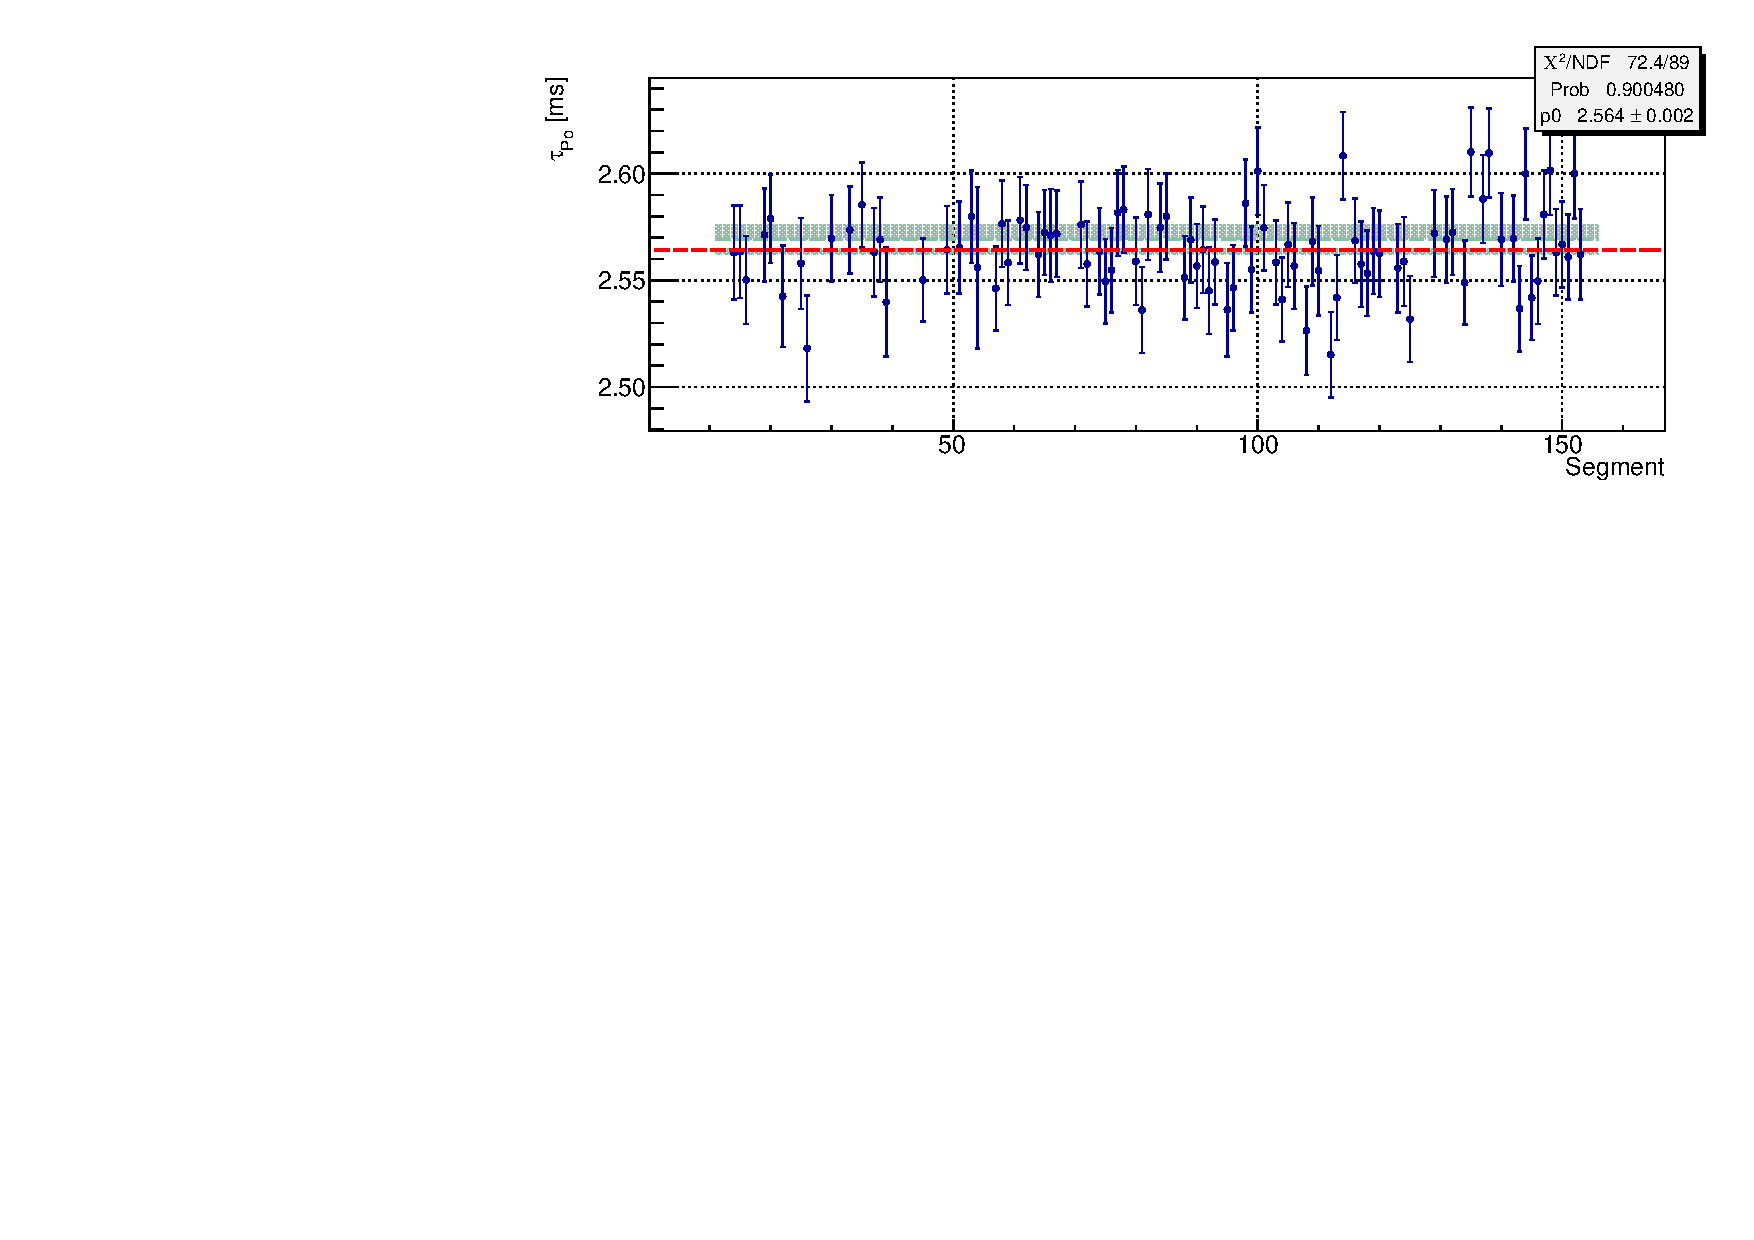
\includegraphics[width=0.8\linewidth]{tex/6-ac227-images/AD_RateCalc/LifetimePerCell}
	\caption{}
	\label{fig:lifetimepercell}
\end{subfigure}
\begin{subfigure}{1\linewidth}
	\centering
	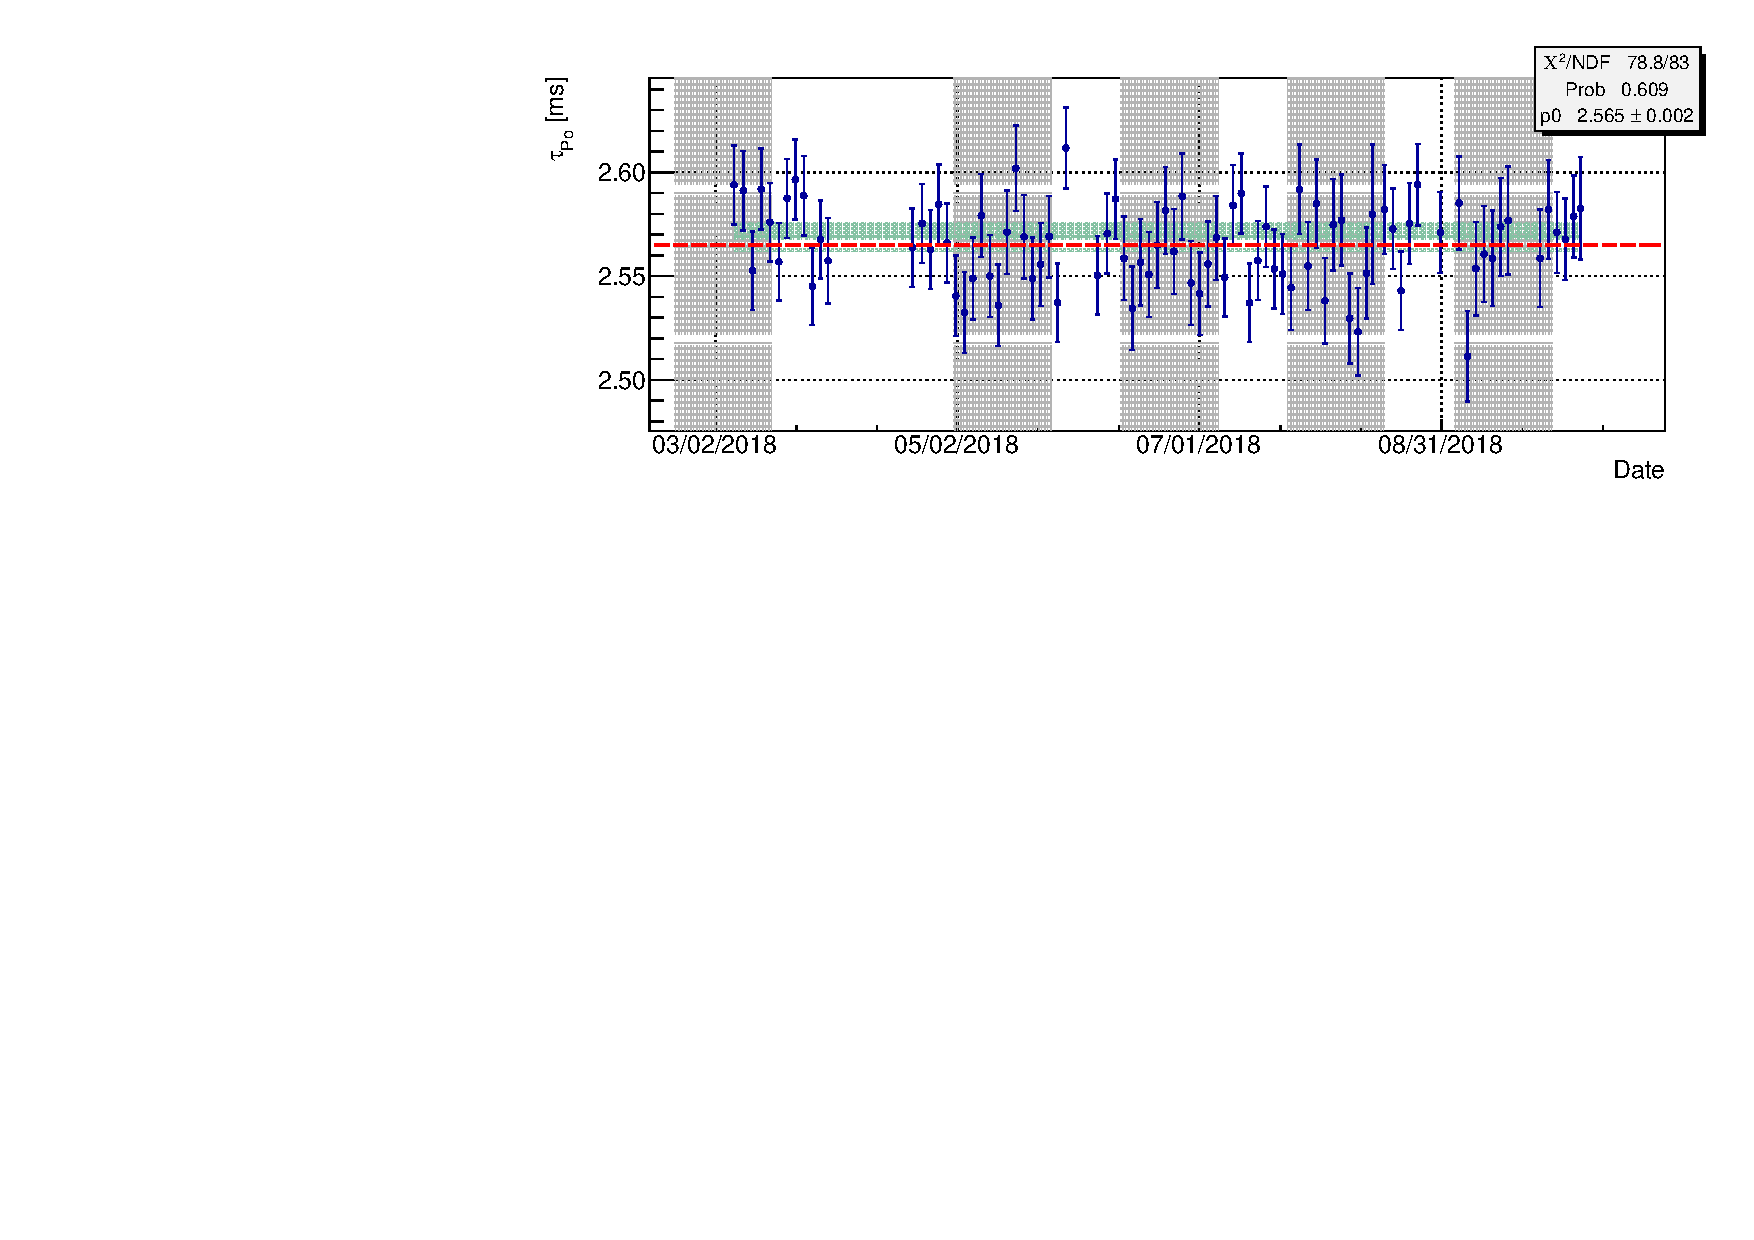
\includegraphics[width=0.8\linewidth]{tex/6-ac227-images/AD_RateCalc/LifetimeVsTime}
	\caption{}
	\label{fig:lifetimevstime}
\end{subfigure}
\caption{The value of $\tau$ obtained from the exponential fit to the $\Delta t$ distribution for each individual segment integrated over all time (a) and for all segments versus time (b). The currently accepted value for $\tau$, 2.569 $\pm$ 0.007 ms, is marked by the shaded green area. A constant fit to the data is shown as the dashed red line. Shaded gray regions in time are reactor on periods.}
\label{fig:tau}
\end{figure}

The uncorrected livetime is calculated, for each data run, as the time from the beginning of the run to the time of the last delay candidate event. 
This is summed for all analyzed runs. 
This livetime was corrected for the dead time introduced by the pileup veto.
This correction was calculated as the number of clusters, $NClusts$, times the pileup veto time, 800 ns.
Figure~\ref{fig:vetotimevstime} shows the dead time, as a fraction of livetime, versus time.
Because the veto was applied to both prompt and delay candidates the livetime is corrected with 2$\times$ the dead time as
\begin{equation}
	\textrm{livetime} = \sum(t_{\textrm{finalPo}} - t_0) - 2.0 \times NClusts \times 800\textrm{ns}
\end{equation}
When measuring the rate per segment the same livetime was applied to all segments. 

\begin{figure}[!t]
	\centering
	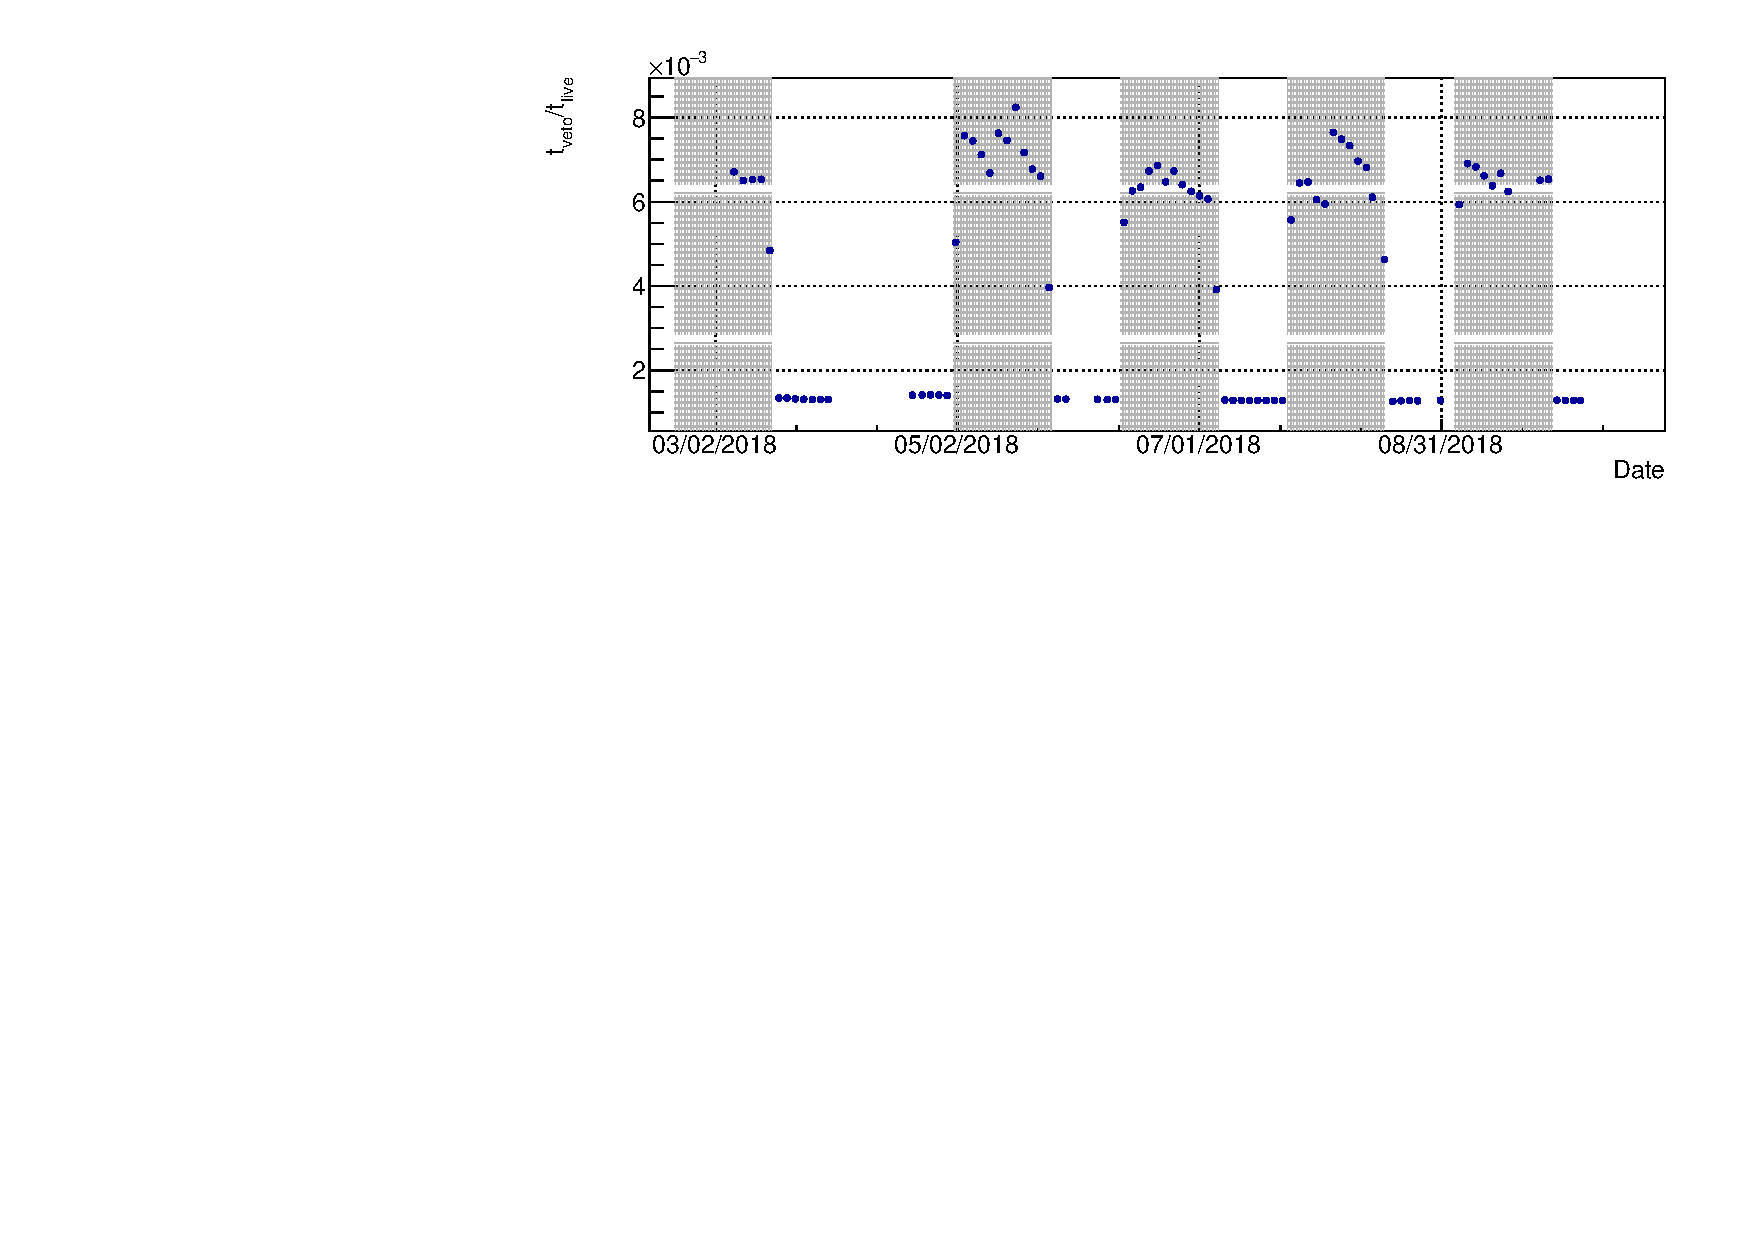
\includegraphics[width=0.8\linewidth]{tex/6-ac227-images/AD_RateCalc/VetoTimeVsTime}
	\caption{The dead time, as a fraction of livetime, due to the pileup veto versus time. Shaded areas are reactor on periods.}
	\label{fig:vetotimevstime}
\end{figure}

The efficiency was calculated for energy and PSD cuts on both prompt and delay events, and for the $\Delta z$ cut.
This was done by fitting each distribution with a Gaussian $\pm 2\sigma$ from the mean.
This is true for all distributions expect the prompt energy, which has a non-Gaussian high energy tail due to its accompanying gammas, see Figure~\ref{fig:rnpoenseg76}. 
Since the high energy cut was always wide enough to include the whole range of this tail, we only care about the low energy cut, which we can approximate with a Gaussian.
Therefore, prompt energy was fit with a Gaussian from -1.3$\sigma$ to +0.6$\sigma$.
The efficiency was then calculated as the ratio of the integral of the Gaussian
between the cuts for that distribution to the integral between $\pm \infty$, as defined in Equation~\ref{eq:Eff}.
The error on the efficiency was treated as a binomial error.
For an example of the distributions and fits for a typical segment see Figure~\ref{fig:RnPoDist}.

\begin{align}
	\text{Eff} = \frac{\int_{\text{low-cut}}^{\text{high-cut}}g(u) du}{\int_{-\infty}^{\infty}g(u) du}
	&& \sigma_{\text{Eff}} =\sqrt{\frac{\text{Eff}(1-\text{Eff})}{N}}
	\label{eq:Eff}
\end{align}	

In general the total efficiency was 99.9\% or higher, for RnPo rates calculated in individual segments and versus time.
Figures~\ref{fig:efficiencypercell} and \ref{fig:efficiencyvstime} show the efficiency calculated for all distributions for all individual segments and versus time, respectively.
See Table~\ref{tab:Cuts} for a summary of all cuts and their average efficiencies.

\begin{figure}[H]
	\begin{subfigure}{0.5\linewidth}
	\centering
	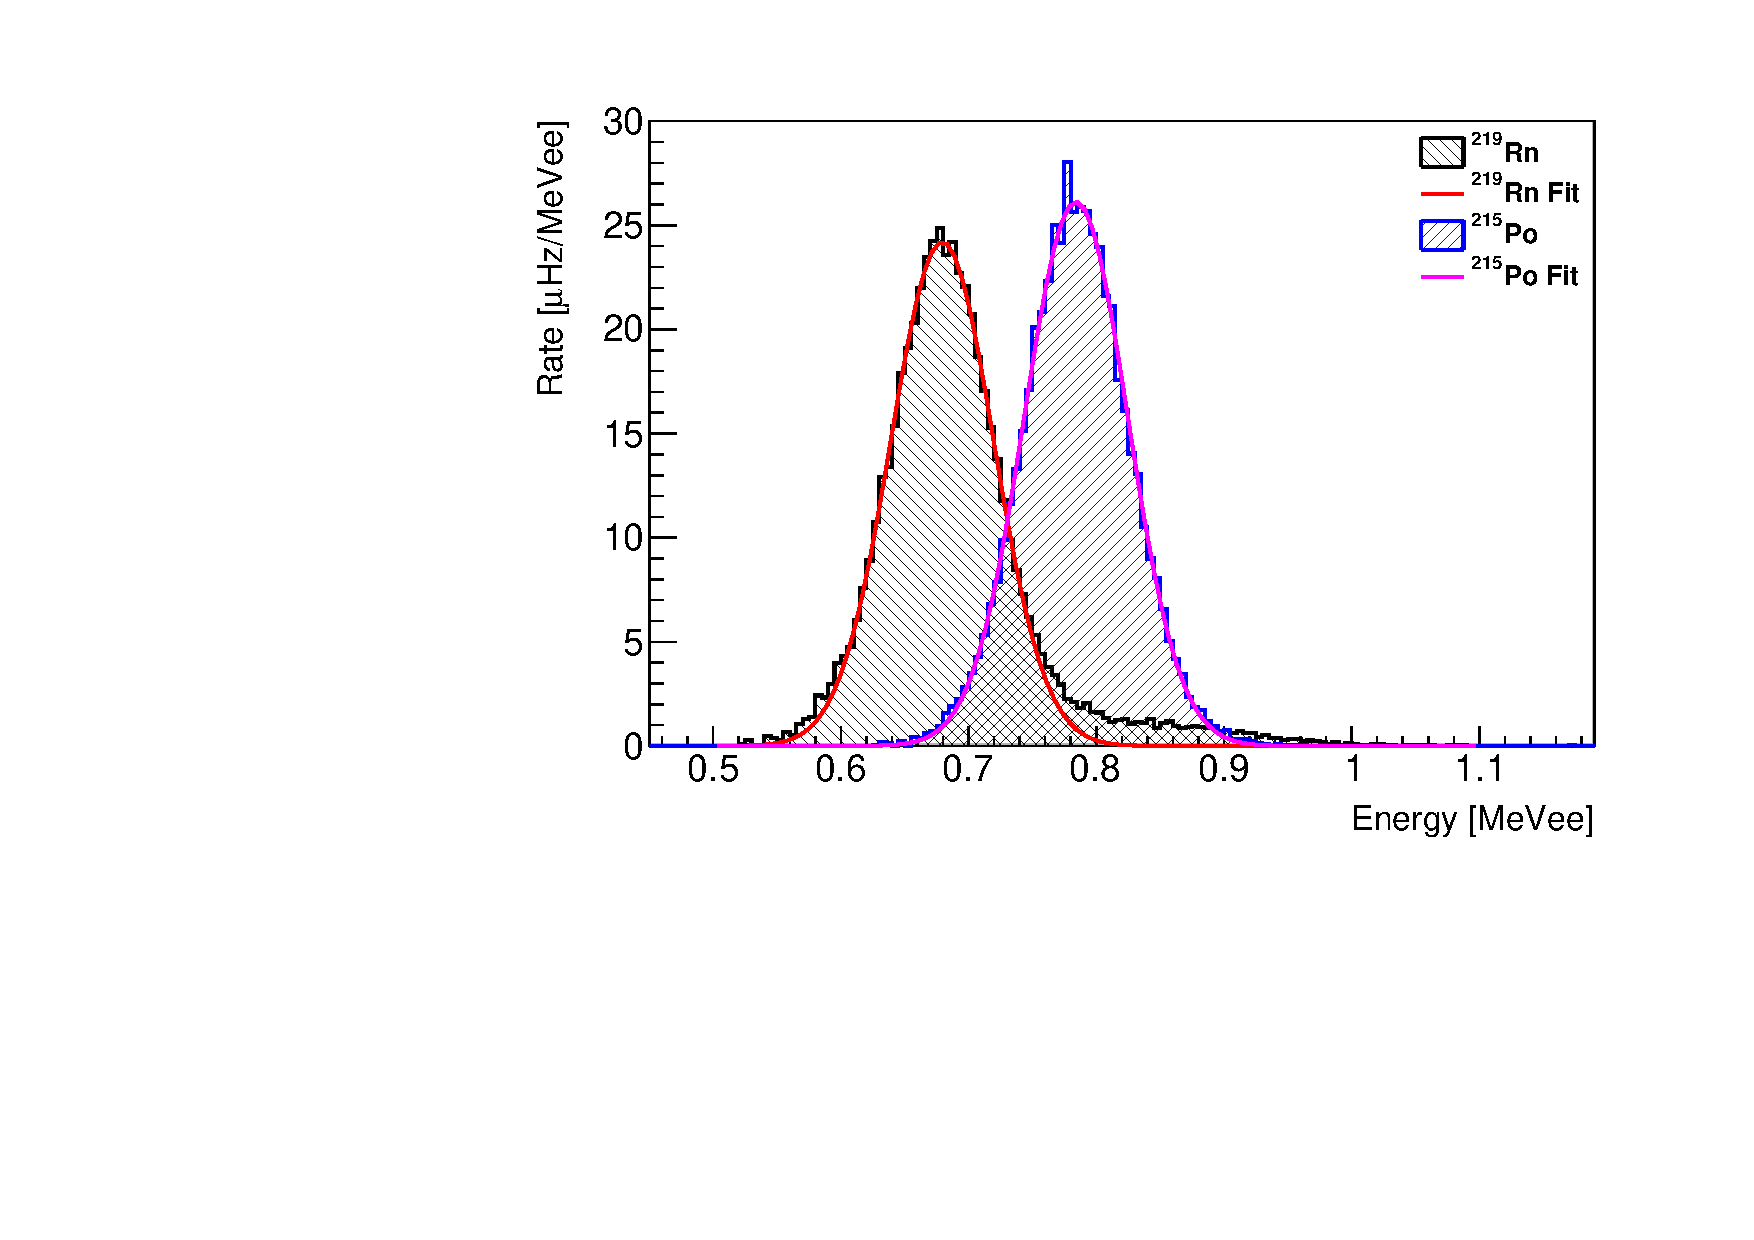
\includegraphics[width=0.95\linewidth]{tex/6-ac227-images/AD_RateCalc/RnPoEn_Seg76}
	\caption{}
	\label{fig:rnpoenseg76}
\end{subfigure}%
\begin{subfigure}{0.5\linewidth}
	\centering
	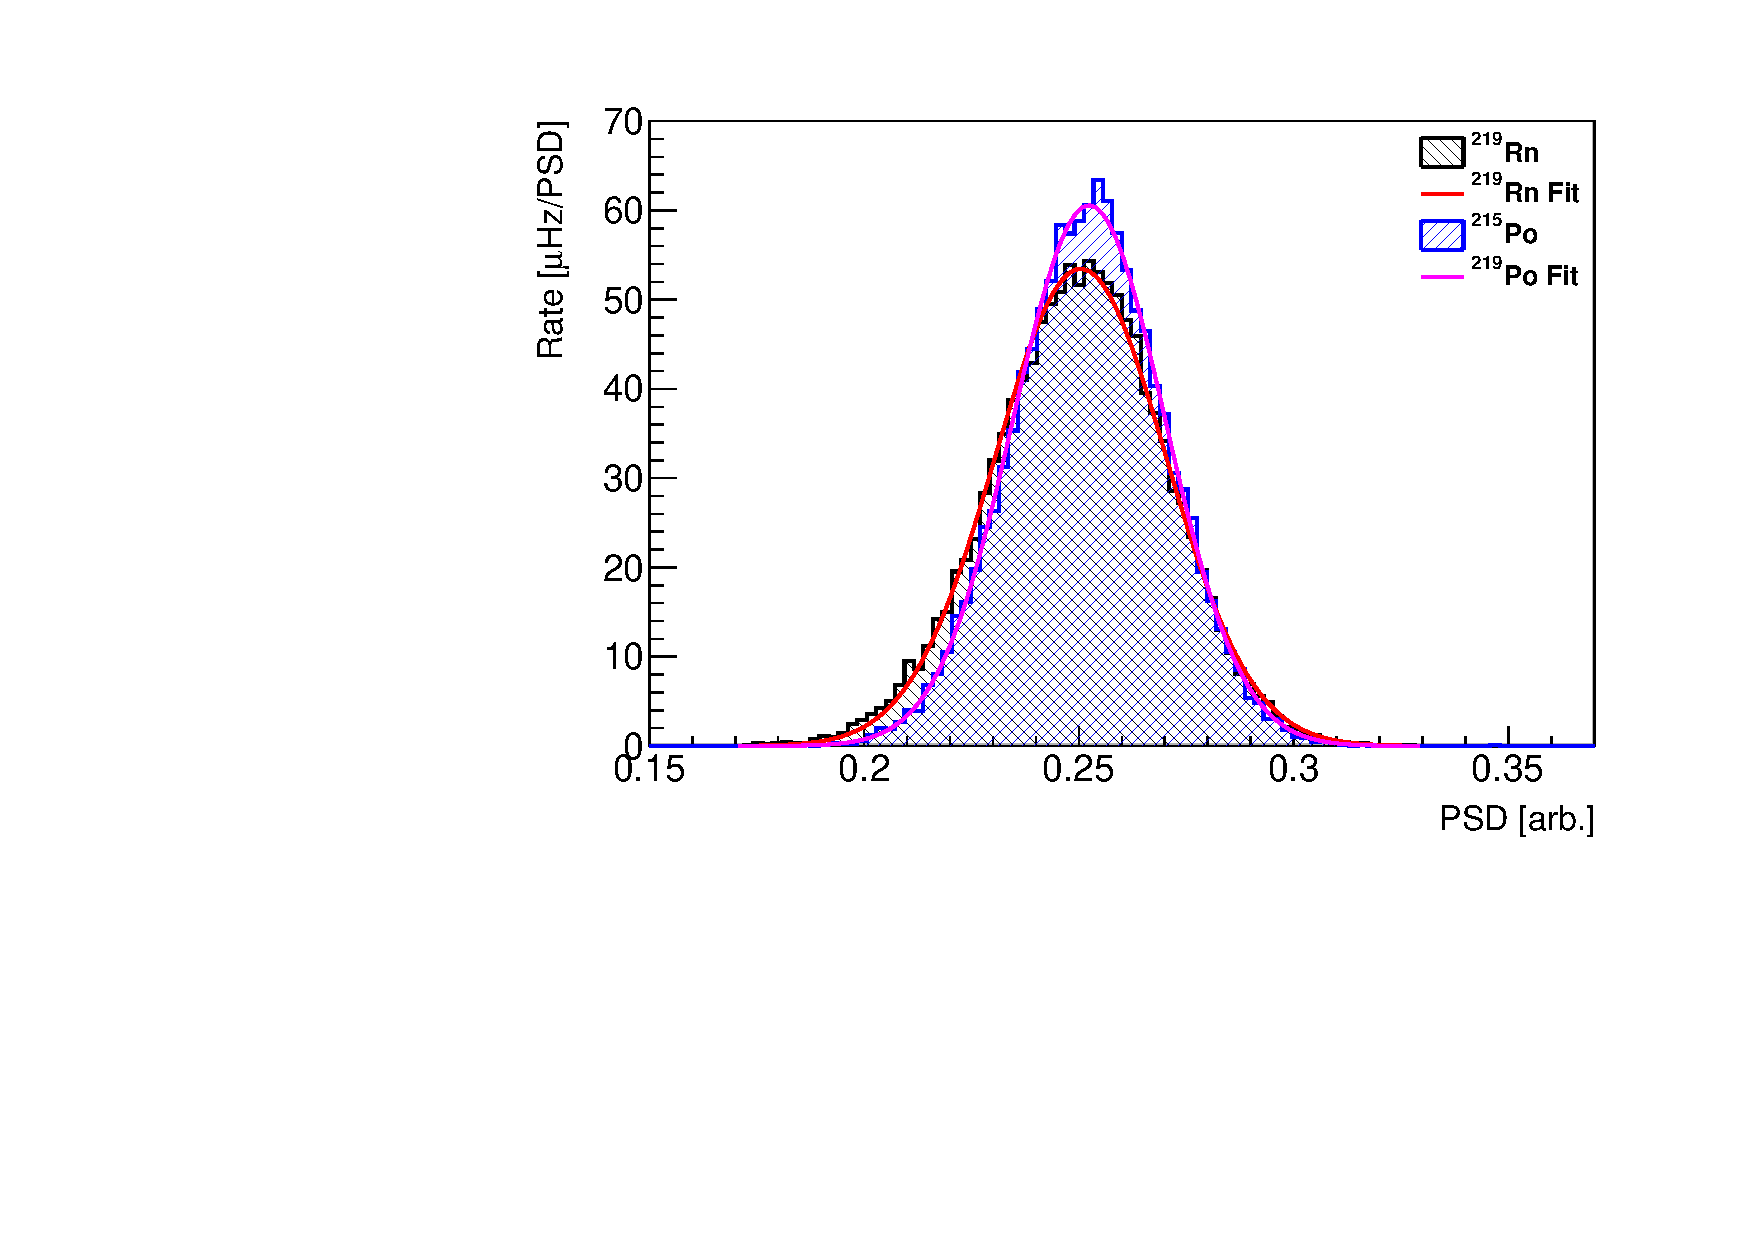
\includegraphics[width=0.95\linewidth]{tex/6-ac227-images/AD_RateCalc/RnPoPSD_Seg76}
	\caption{}
	\label{fig:rnpopsdseg76}
\end{subfigure}
\begin{subfigure}{1\linewidth}
	\centering
	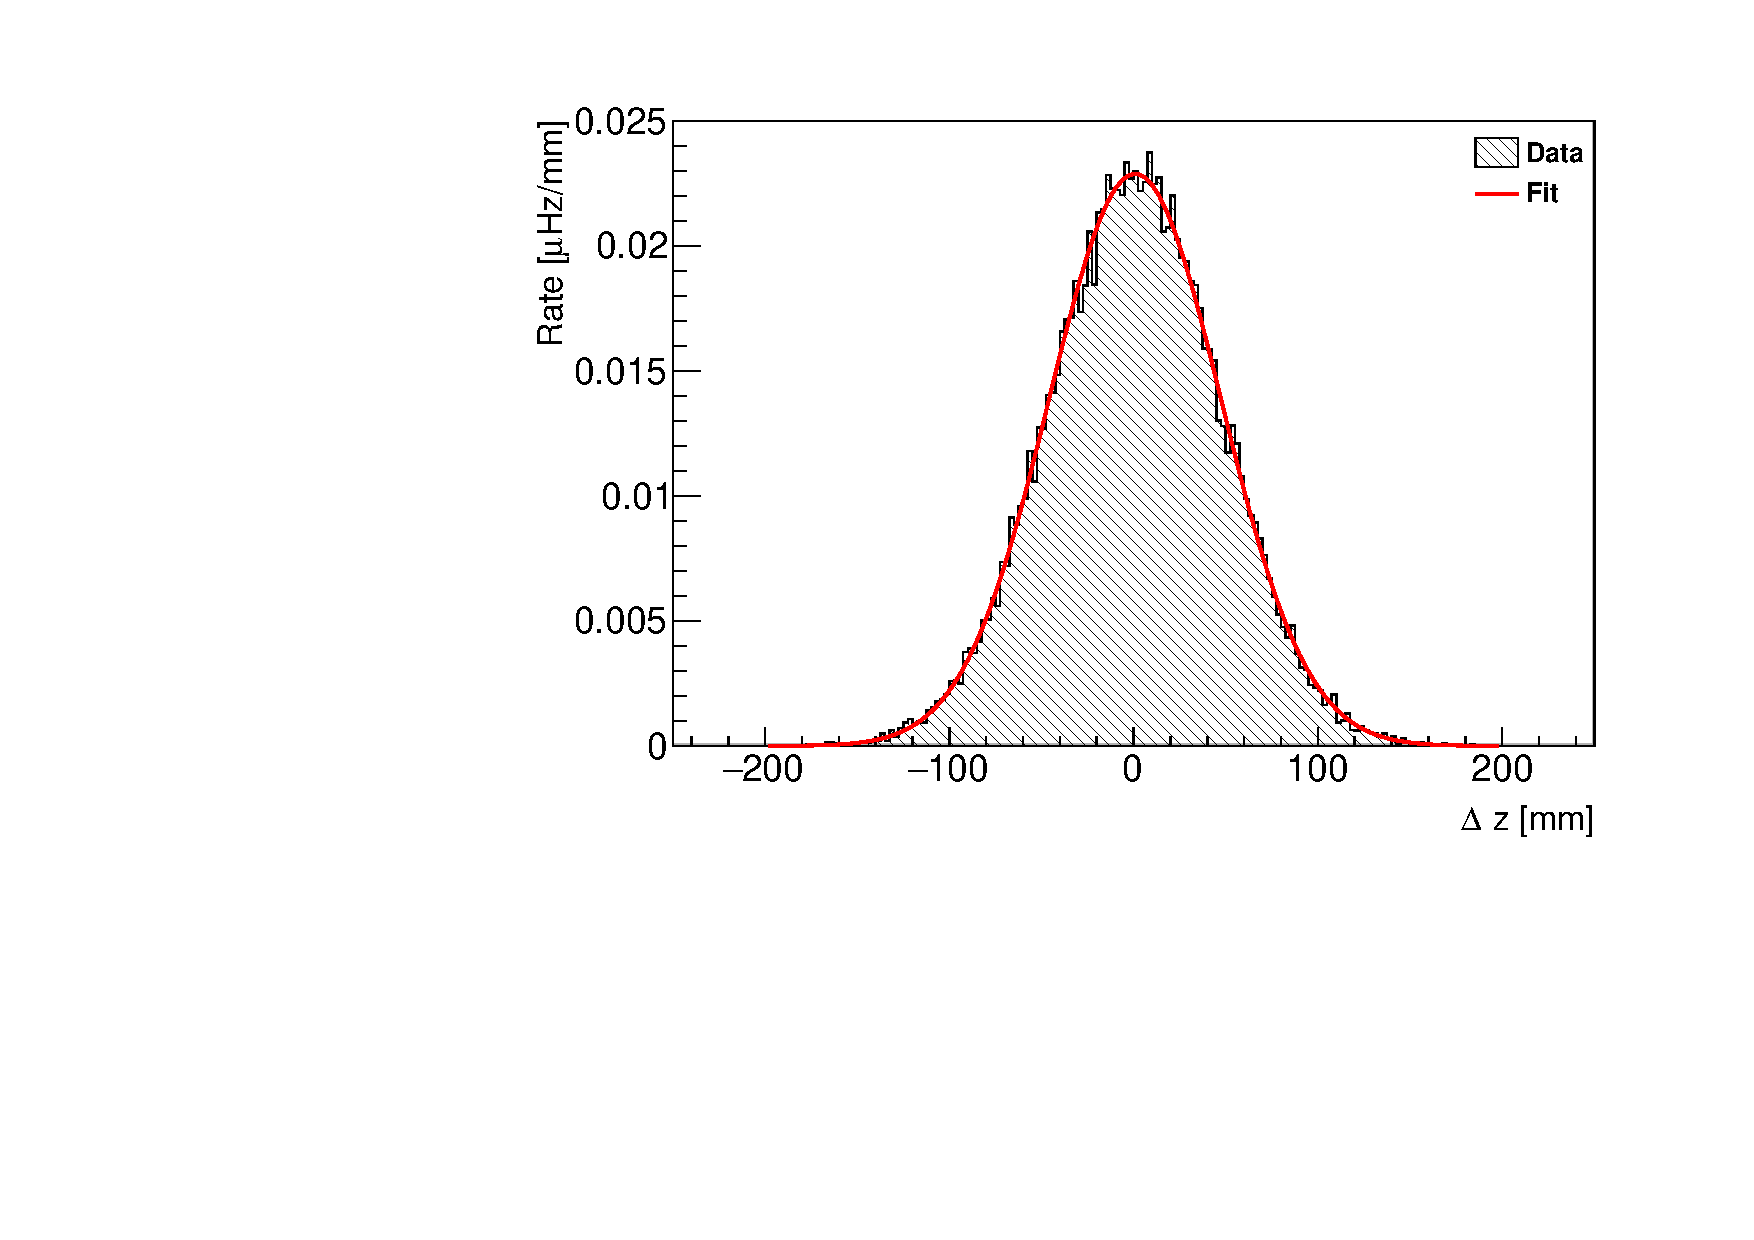
\includegraphics[width=0.475\linewidth]{tex/6-ac227-images/AD_RateCalc/RnPoDz_Seg76}
	\caption{}
	\label{fig:rnpodzseg76}
\end{subfigure}
\caption{Energy (a), PSD (b), and $\Delta z$ (c) distributions for RnPo events in a typical segment integrated over all time. Also shown are the results of fitting each distribution with a Gaussian for the purpose of calculating the cut efficiencies.}
\label{fig:RnPoDist}
\end{figure}

\begin{figure}[h]
	\centering
	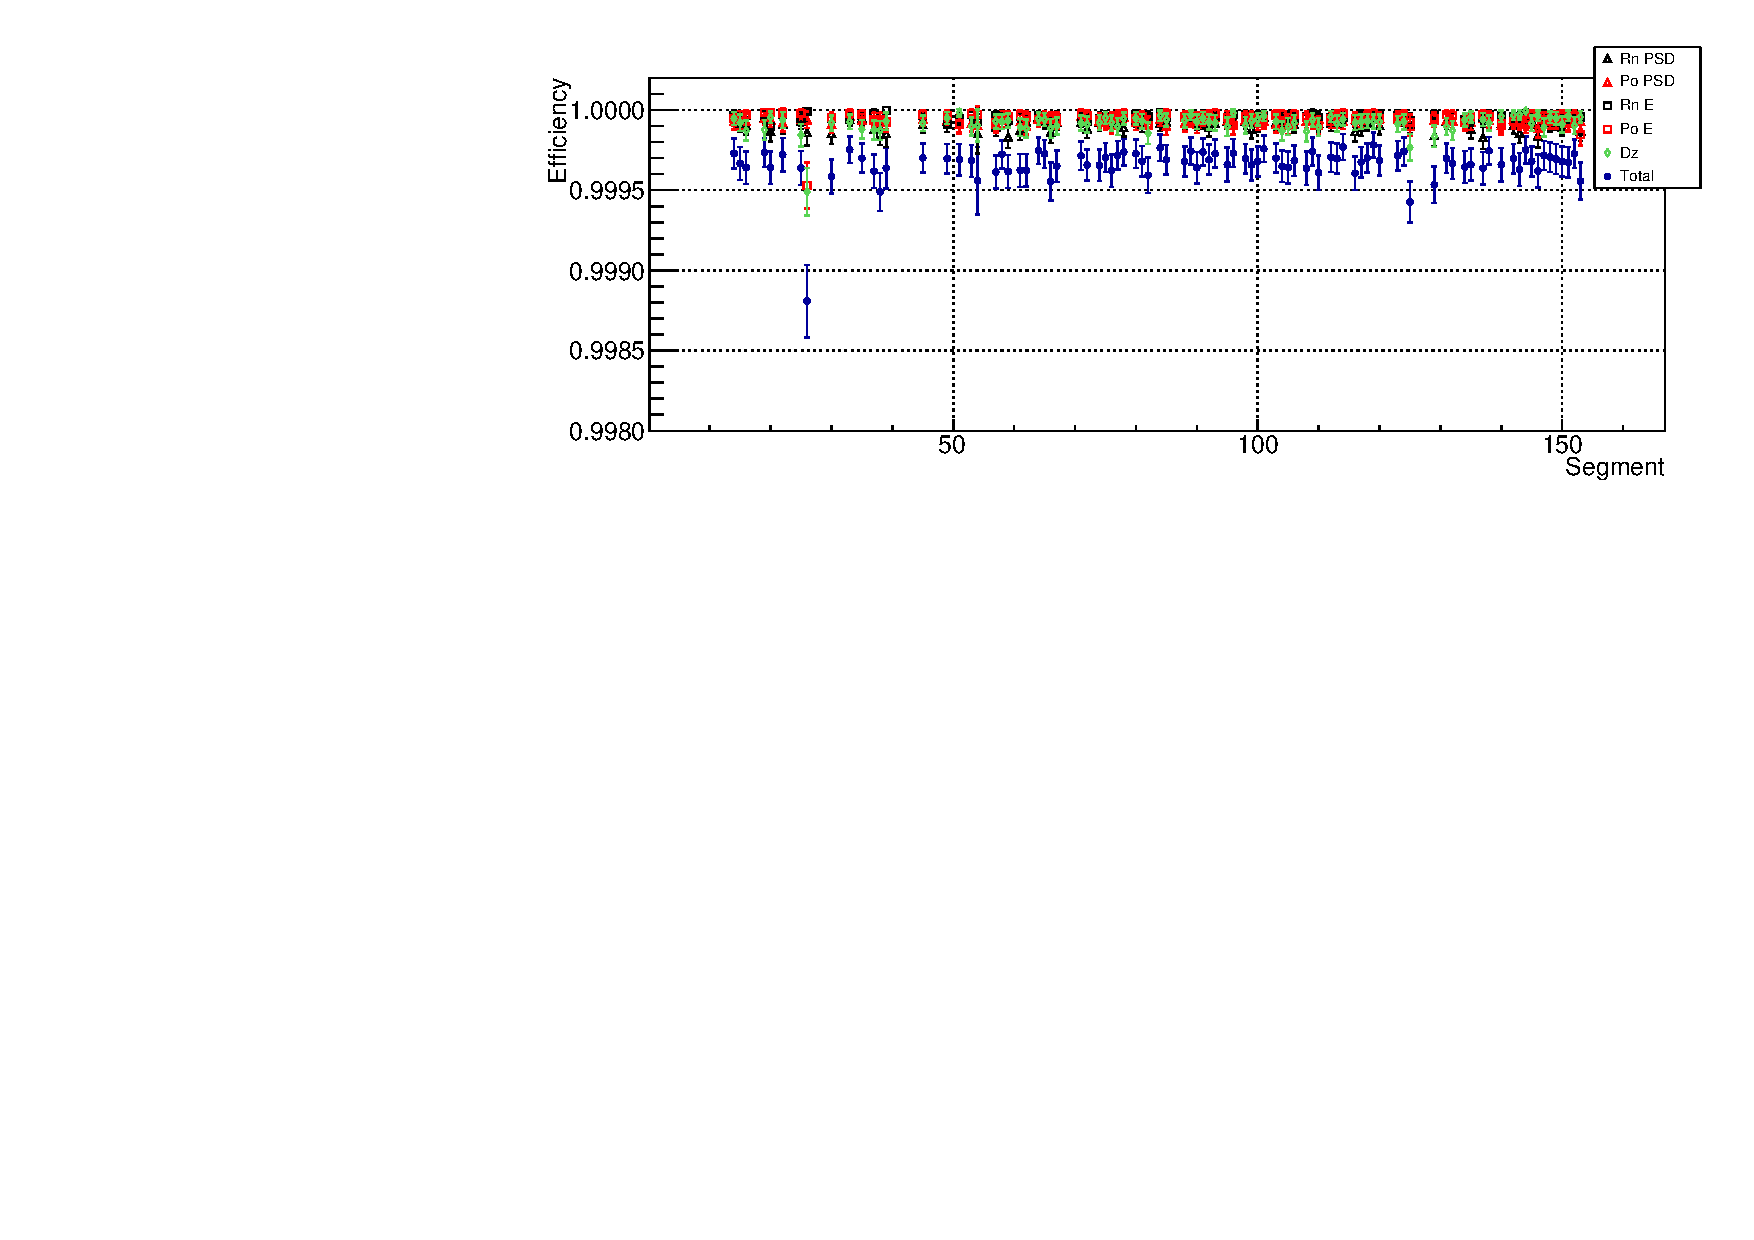
\includegraphics[width=0.9\linewidth]{tex/6-ac227-images/AD_RateCalc/EfficiencyPerCell}
	\caption{Cut efficiencies calculated for RnPo events in individual segments integrated over all time.}
	\label{fig:efficiencypercell}
\end{figure}

\begin{figure}[h]
	\centering
	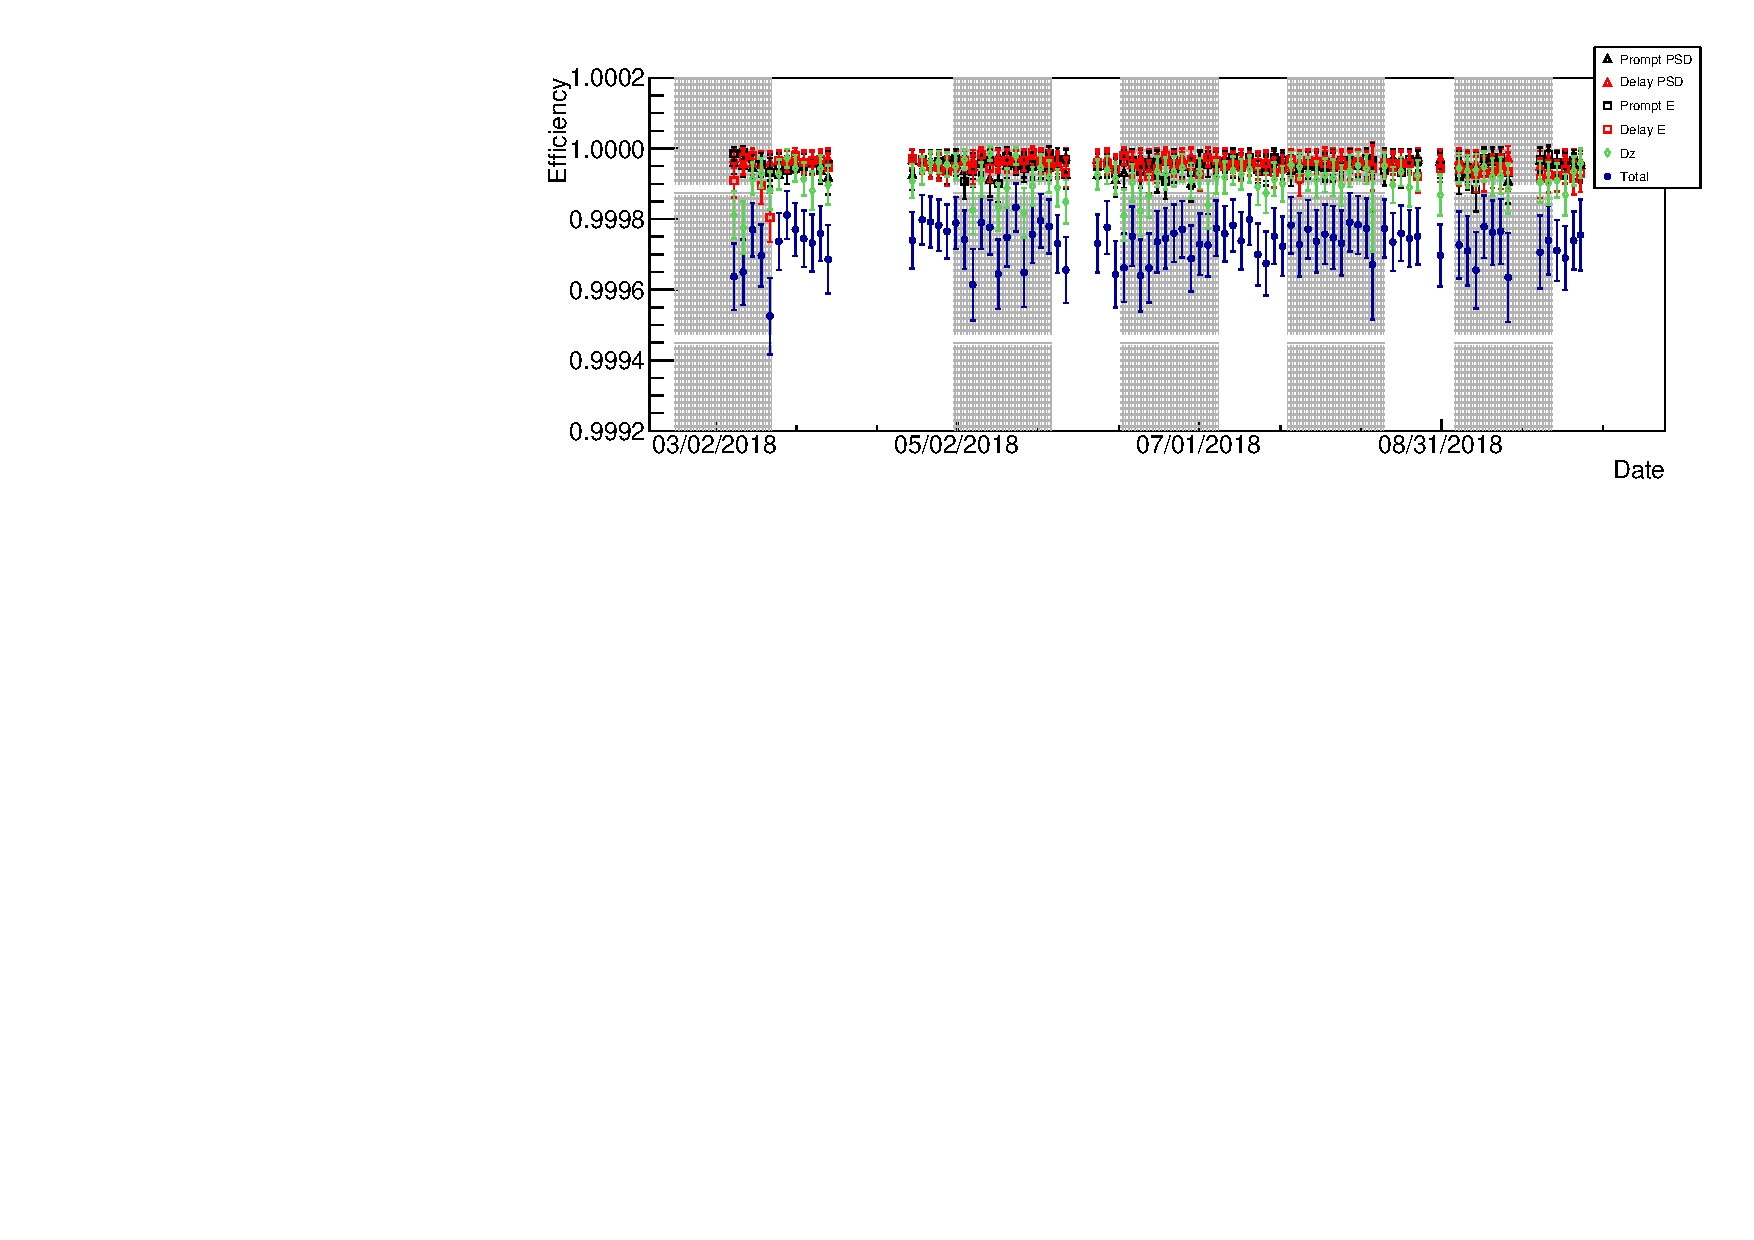
\includegraphics[width=0.9\linewidth]{tex/6-ac227-images/AD_RateCalc/EfficiencyVsTime}
	\caption{Cut efficiencies calculated for RnPo events versus time integrated over all segments. Shaded areas are reactor on periods.}
	\label{fig:efficiencyvstime}
\end{figure}

\begin{table}[H]
	\centering
	\begin{tabular}{c|c|c|c}
		\hline
		\textbf{Cut}         & \textbf{Range} & \textbf{$\langle$Eff$_{\text{Cell}}\rangle$\%} & \textbf{$\langle$Eff$_{\text{Time}}\rangle$\%} \\ \hline
		Pileup veto & Veto any cluster preceded             &   & \\ 
		& less than 800 ns by another cluster   &   & \\ \hline
		PSD         & $\mu - 4\sigma < \text{PSD}_{\text{Rn}} <$ 0.36 & 99.993  & 99.996 \\ 
		& $\mu - 4\sigma < \text{PSD}_{\text{Po}} <$ 0.36 & 99.994  & 99.997 \\ \hline
		Energy      & $\mu - 4\sigma < \text{E}_{\text{Rn}} <$ 1.18 MeV & 99.997  & 99.996  \\
		& $\mu - 4\sigma < \text{E}_{\text{Po}} <$ 1.18 MeV & 99.996  & 99.996 \\ \hline
		Position    & -1000 $< \text{z}_{\text{Rn/Po}} <$ 1000 mm &    &   \\ 
		& Segment-Rn = Segment-Po & & \\ \hline
		$\Delta$z   & $\mu - 4\sigma < \Delta \text{z} < \mu + 4\sigma$   & 99.994   & 99.993  \\ \hline
		$\Delta$t   & $0.5 < \Delta \text{t} < 12.845$ ms &  &   \\ \hline
	\end{tabular}
	\caption{Summary of the chosen cuts and their average efficiencies for determining the \Ac rate in the PROSPECT AD. The means and sigmas are determined by fitting the peaks of all distributions with Gaussians. They are found for each individual segment or each individual time bin (depending on the analysis being done). Average efficiencies are found by fitting the data in Figures~\ref{fig:efficiencypercell} and \ref{fig:efficiencyvstime} with constants.}
	\label{tab:Cuts}
\end{table}


\subsection{Detector Performance as Tracked with \Ac}

Though \Ac was added to the detector in order to measure relative segment-to-segment volume variations, the mono-energetic \Po $\alpha$ was also useful for tracking the performance of the detector and the applied calibrations.
Figure~\ref{fig:EvsT} shows the mean and 1$\sigma$ width of the \Po energy distribution versus time, integrated over all segments. 
It can be seen that the resolution was not stable over time, but rather decreased by $\sim$20\% over a period of 7 months.
This is due to an overall decrease in light collection over time, implying some factor of scintillator degradation such as a loss of transparency or light production, whose cause is not yet understood.

To correct for this in the IBD analysis a variable called $E_{smear}$ was introduced, in which all energy distributions were smeared by artificially adding random noise at the software level to match the worst resolution in a given data taking period.
The results of this are also shown in Figure~\ref{fig:EvsT}, and it can be seen that the new $E_{smear}$ resolution values were time-stable within $\pm$3\% and the mean values within $\pm$0.4\%.
Note that the sharp variations in the energy mean values correspond to times when a new set of calibration constants were introduced in the analysis.

Though introducing the $E_{smear}$ variable corrected for changing detector characteristics, the \Ac analysis used $E$. 
The decreasing resolution was accounted for by applying $\sigma$-based cuts to the energy.

\begin{figure}[h]
\begin{subfigure}{1\linewidth}
	\centering
	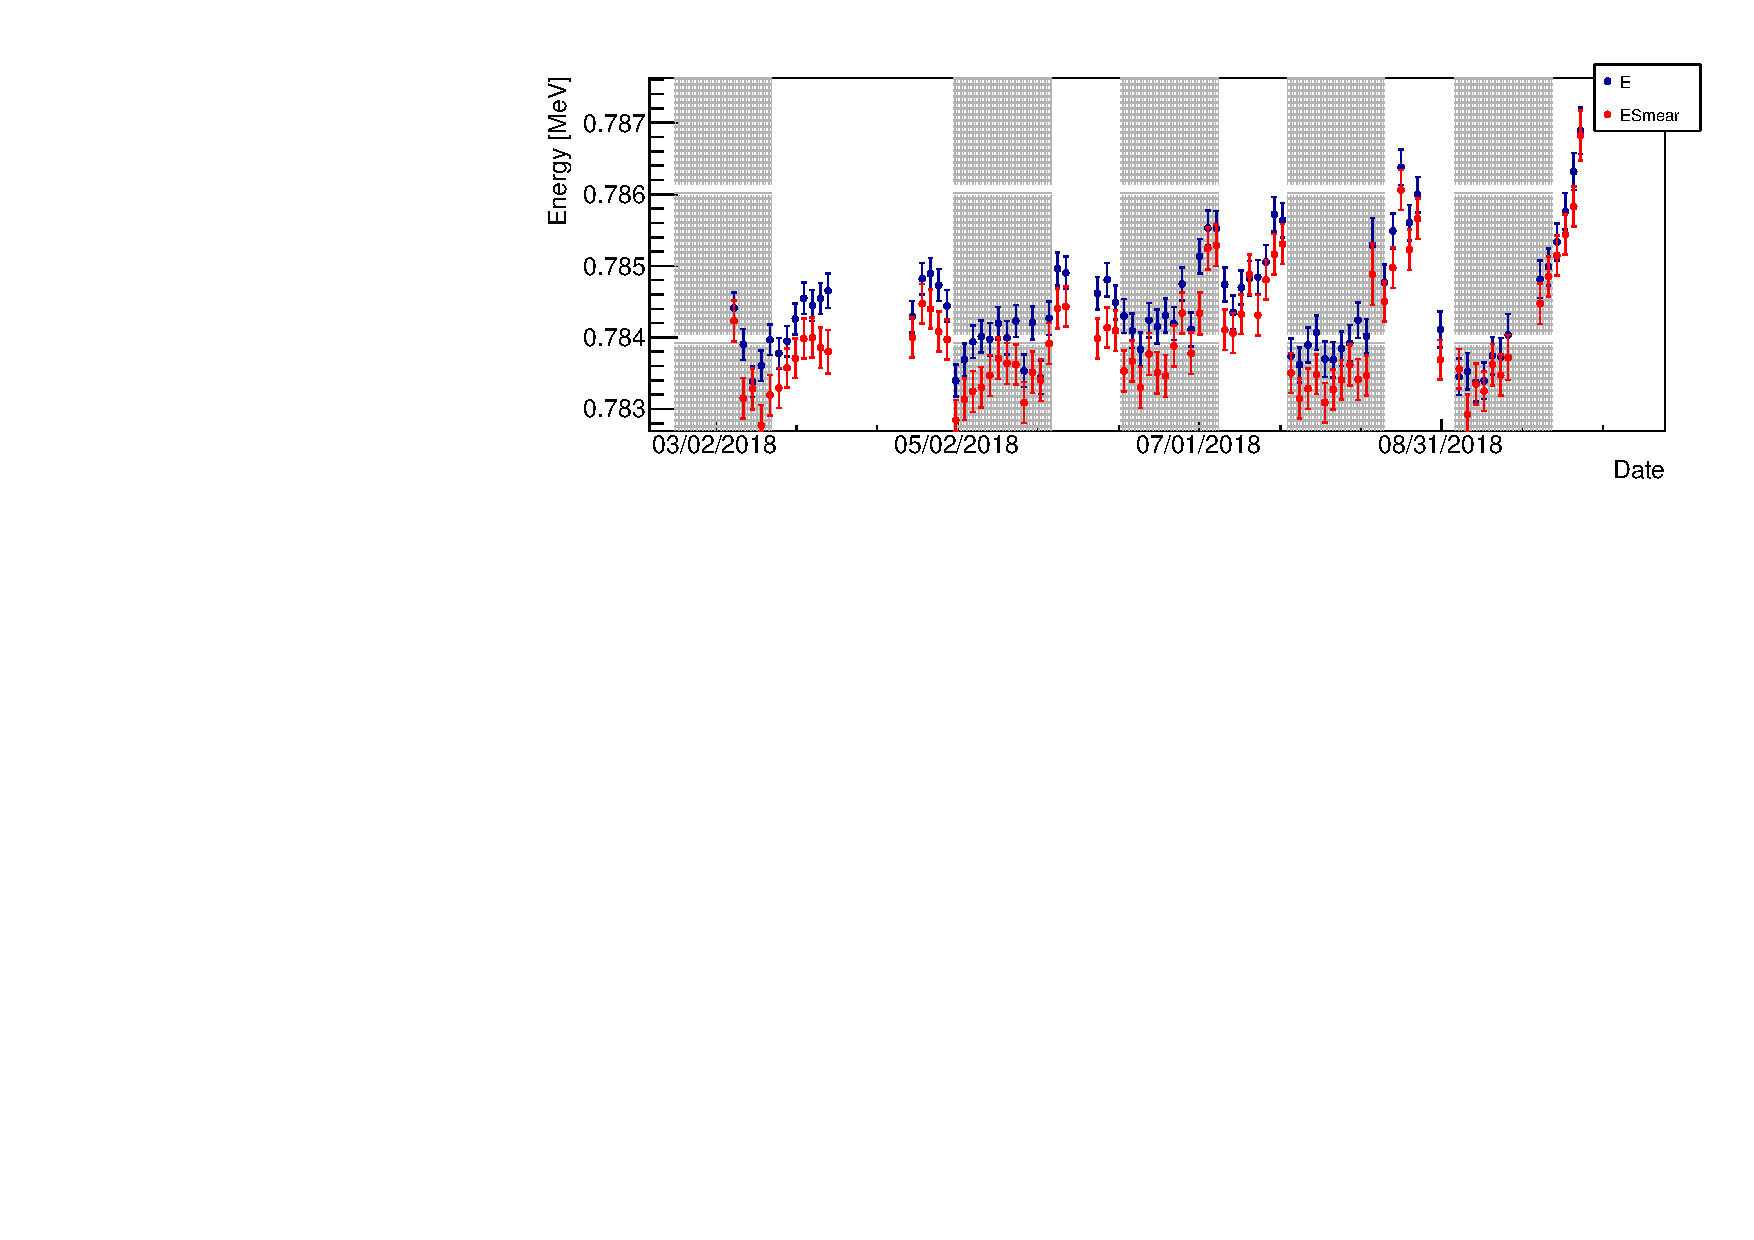
\includegraphics[width=0.9\linewidth]{tex/6-ac227-images/DetPerformance/PoEnMeanVsTime}
	\caption{}
	\label{fig:poenmeanvstime}
\end{subfigure}
\begin{subfigure}{1\linewidth}
	\centering
	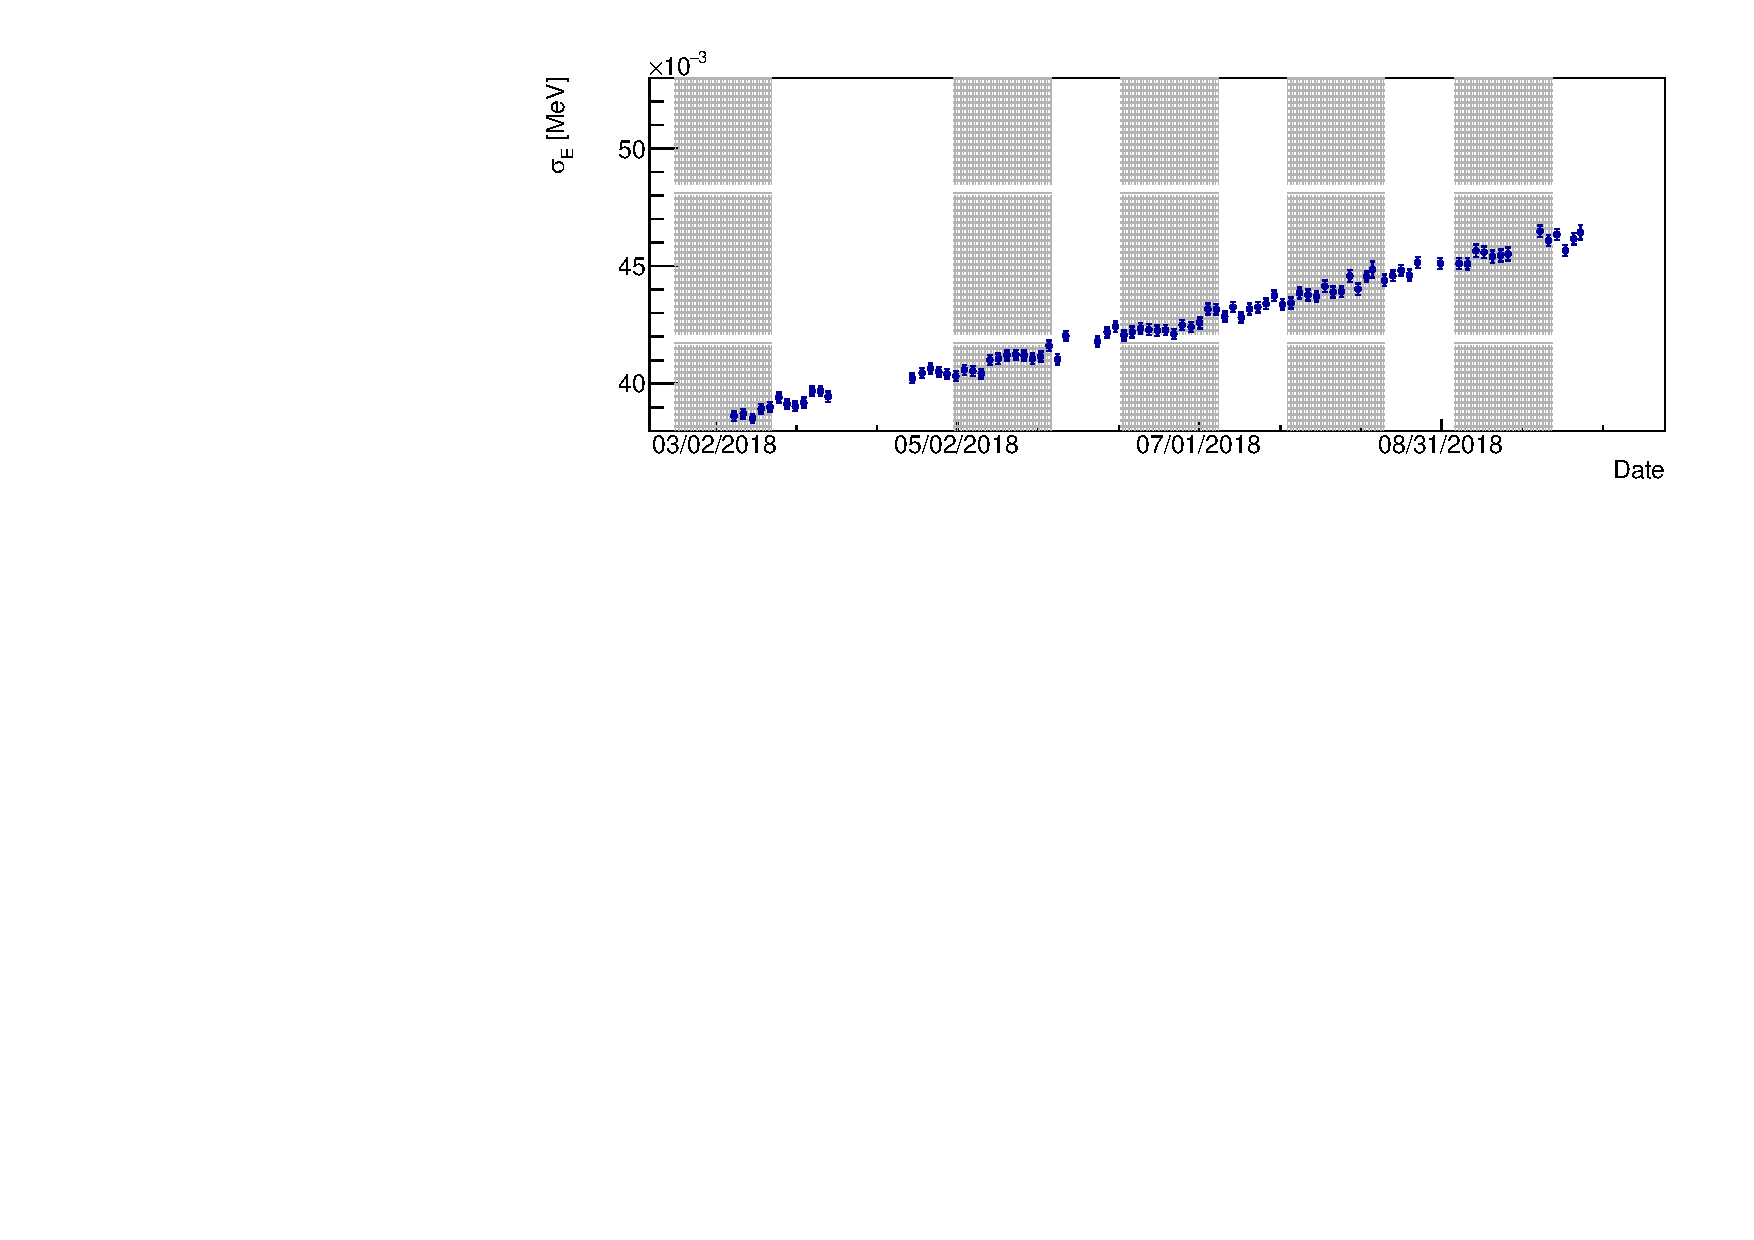
\includegraphics[width=0.9\linewidth]{tex/6-ac227-images/DetPerformance/PoEnSigmaVsTime}
	\caption{}
	\label{fig:poensigmavstime}
\end{subfigure}
\caption{Mean (a) and 1$\sigma$ width (b) of the \Po energy distribution versus time integrated over all segments. Both before applied a correction (E) and after correction (ESmear) are shown. Shaded areas are reactor on periods.}
\label{fig:EvsT}
\end{figure}

The mean and width of the \Po PSD distribution versus time are shown in Figure~\ref{fig:PSDvsT}.
Similar behavior as was seen in the energy distribution also occurs to the PSD.
Over the 7 month period the PSD distribution increases in width by $\sim$11\% as the mean decreases by $\sim$9\%.
This is accounted for the \Ac analysis by the use of $\sigma$-based cuts on the PSD distributions.

\begin{figure}[h]
\begin{subfigure}{1\linewidth}
	\centering
	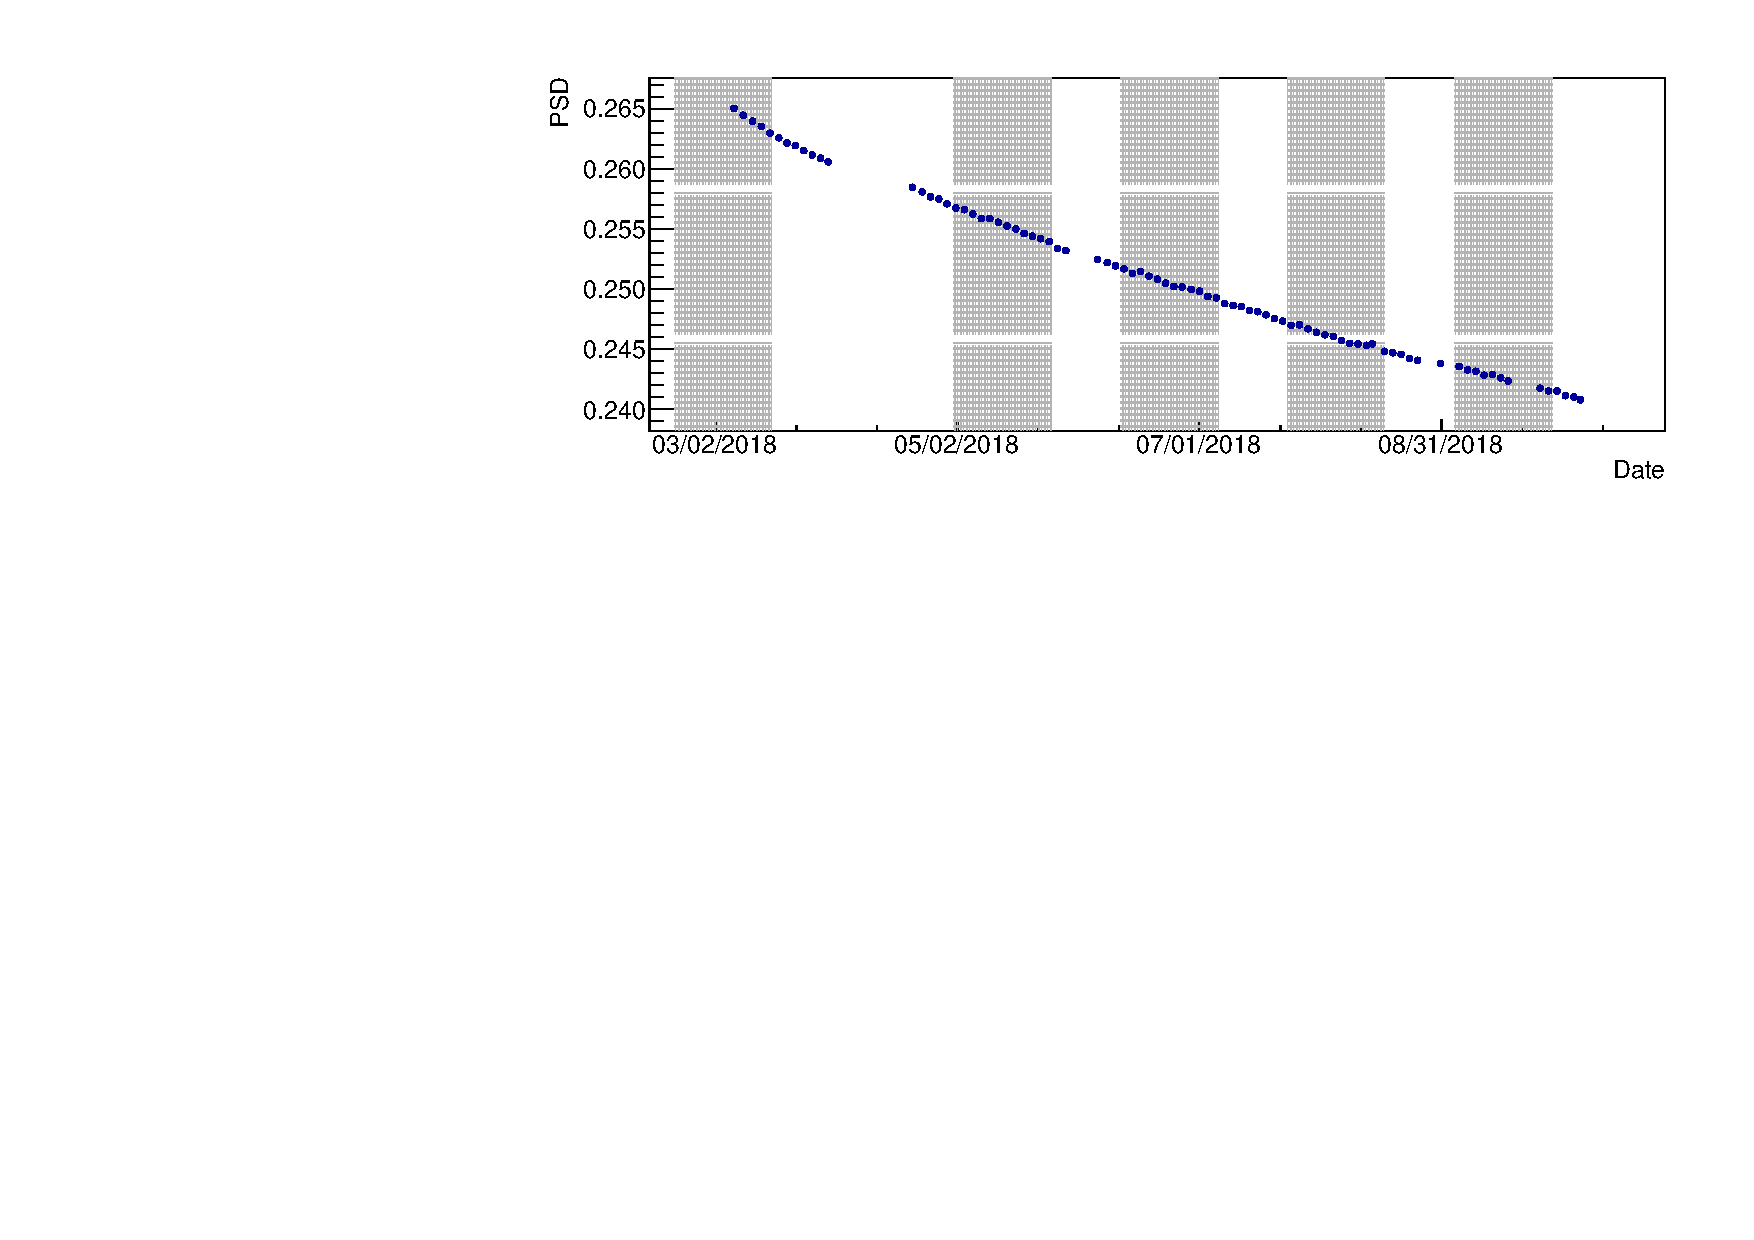
\includegraphics[width=0.9\linewidth]{tex/6-ac227-images/DetPerformance/PoPSDMeanVsTime}
	\caption{}
	\label{fig:popsdmeanvstime}
\end{subfigure}
\begin{subfigure}{1\linewidth}
	\centering
	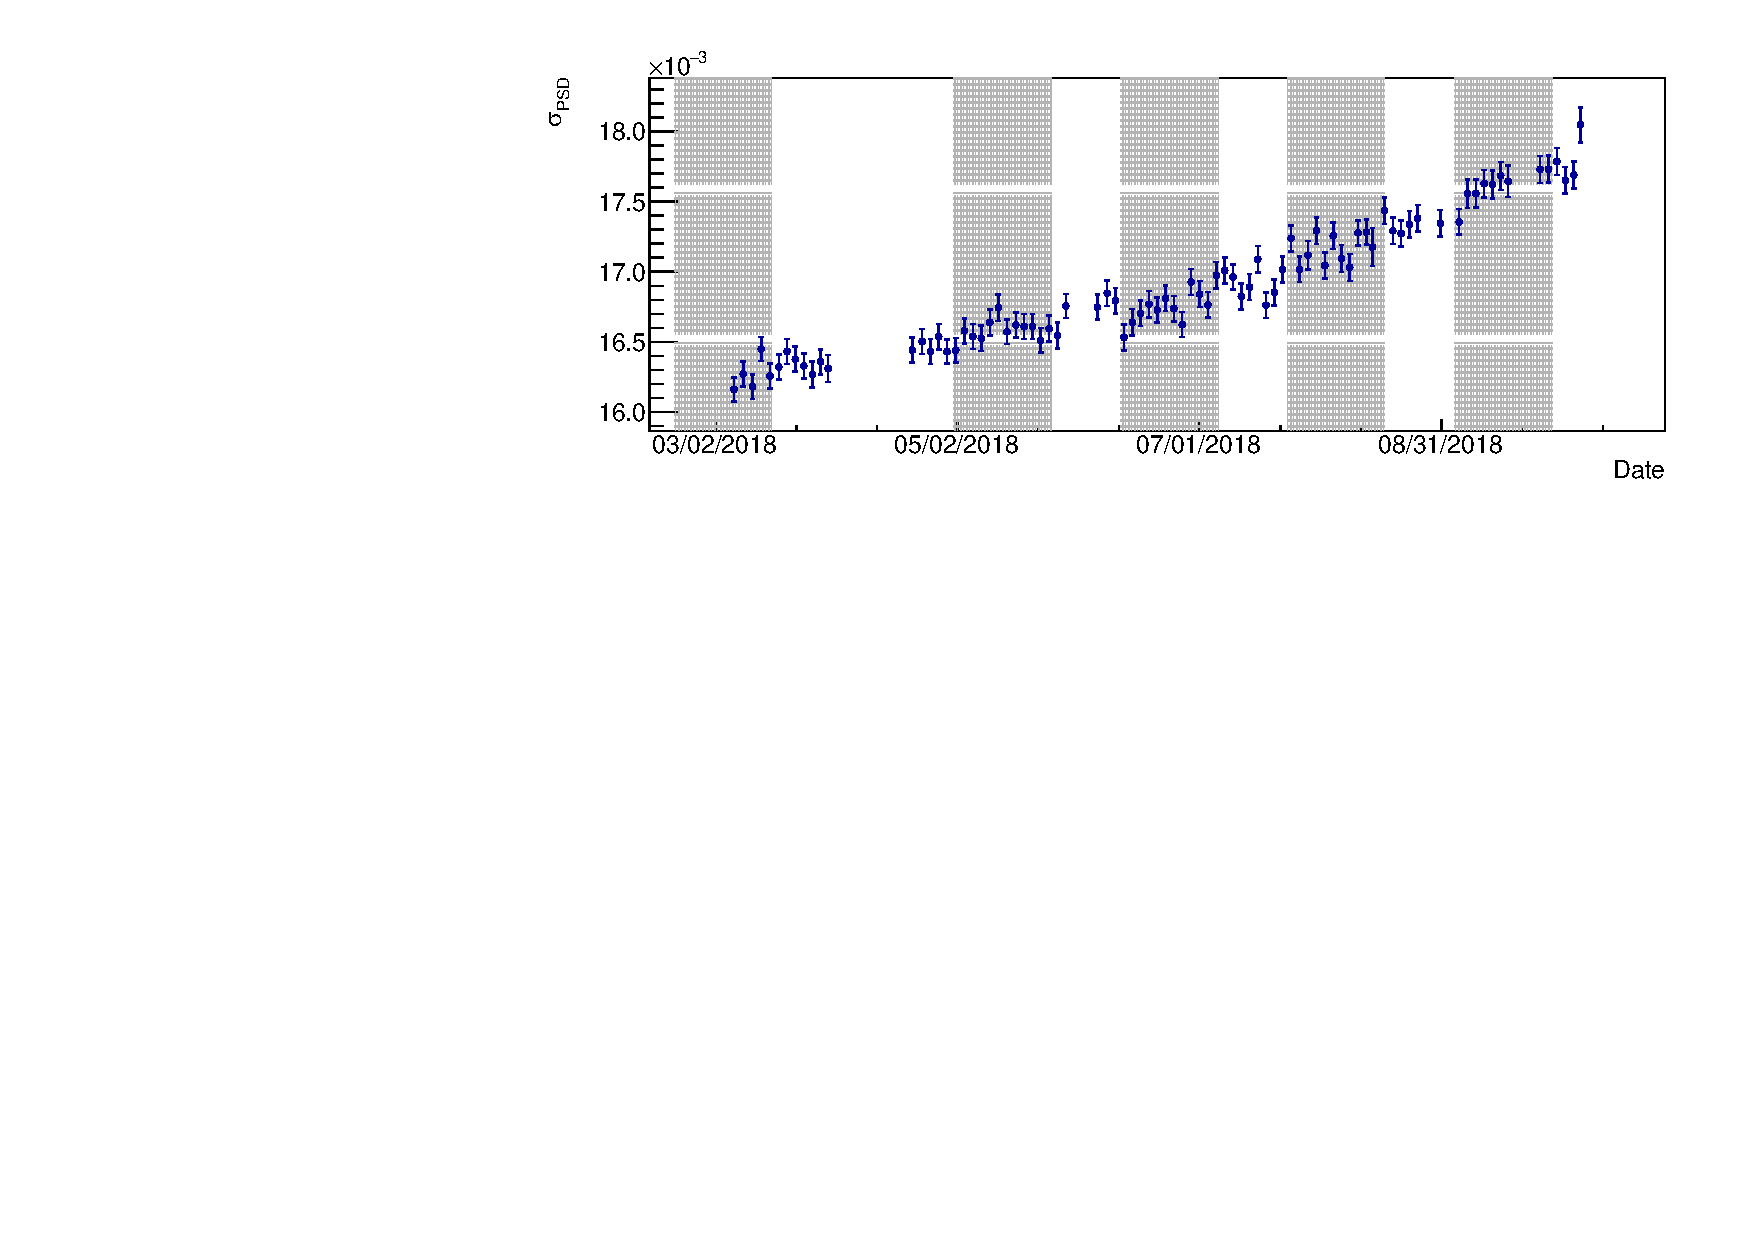
\includegraphics[width=0.9\linewidth]{tex/6-ac227-images/DetPerformance/PoPSDSigmaVsTime}
	\caption{}
	\label{fig:popsdsigmavstime}
\end{subfigure}
\caption{Mean (a) and 1$\sigma$ width (b) of the \Po PSD distribution versus time integrated over all segments. Shaded areas are reactor on periods.}
\label{fig:PSDvsT}
\end{figure}

Position resolution can be determined using the reconstructed position difference of the highly localized coincident alphas.
This is plotted versus time, integrated over all segments, in Figure~\ref{fig:rnpodzsigmavstime}.
It can be seen that the width increases by 7\% over the 7 month period, about 3.5 mm. 
This variation is accounted for in the \Ac analysis in the same way as was done for energy and PSD, by using $\sigma$-based cuts.

\begin{figure}[h]
	\centering
	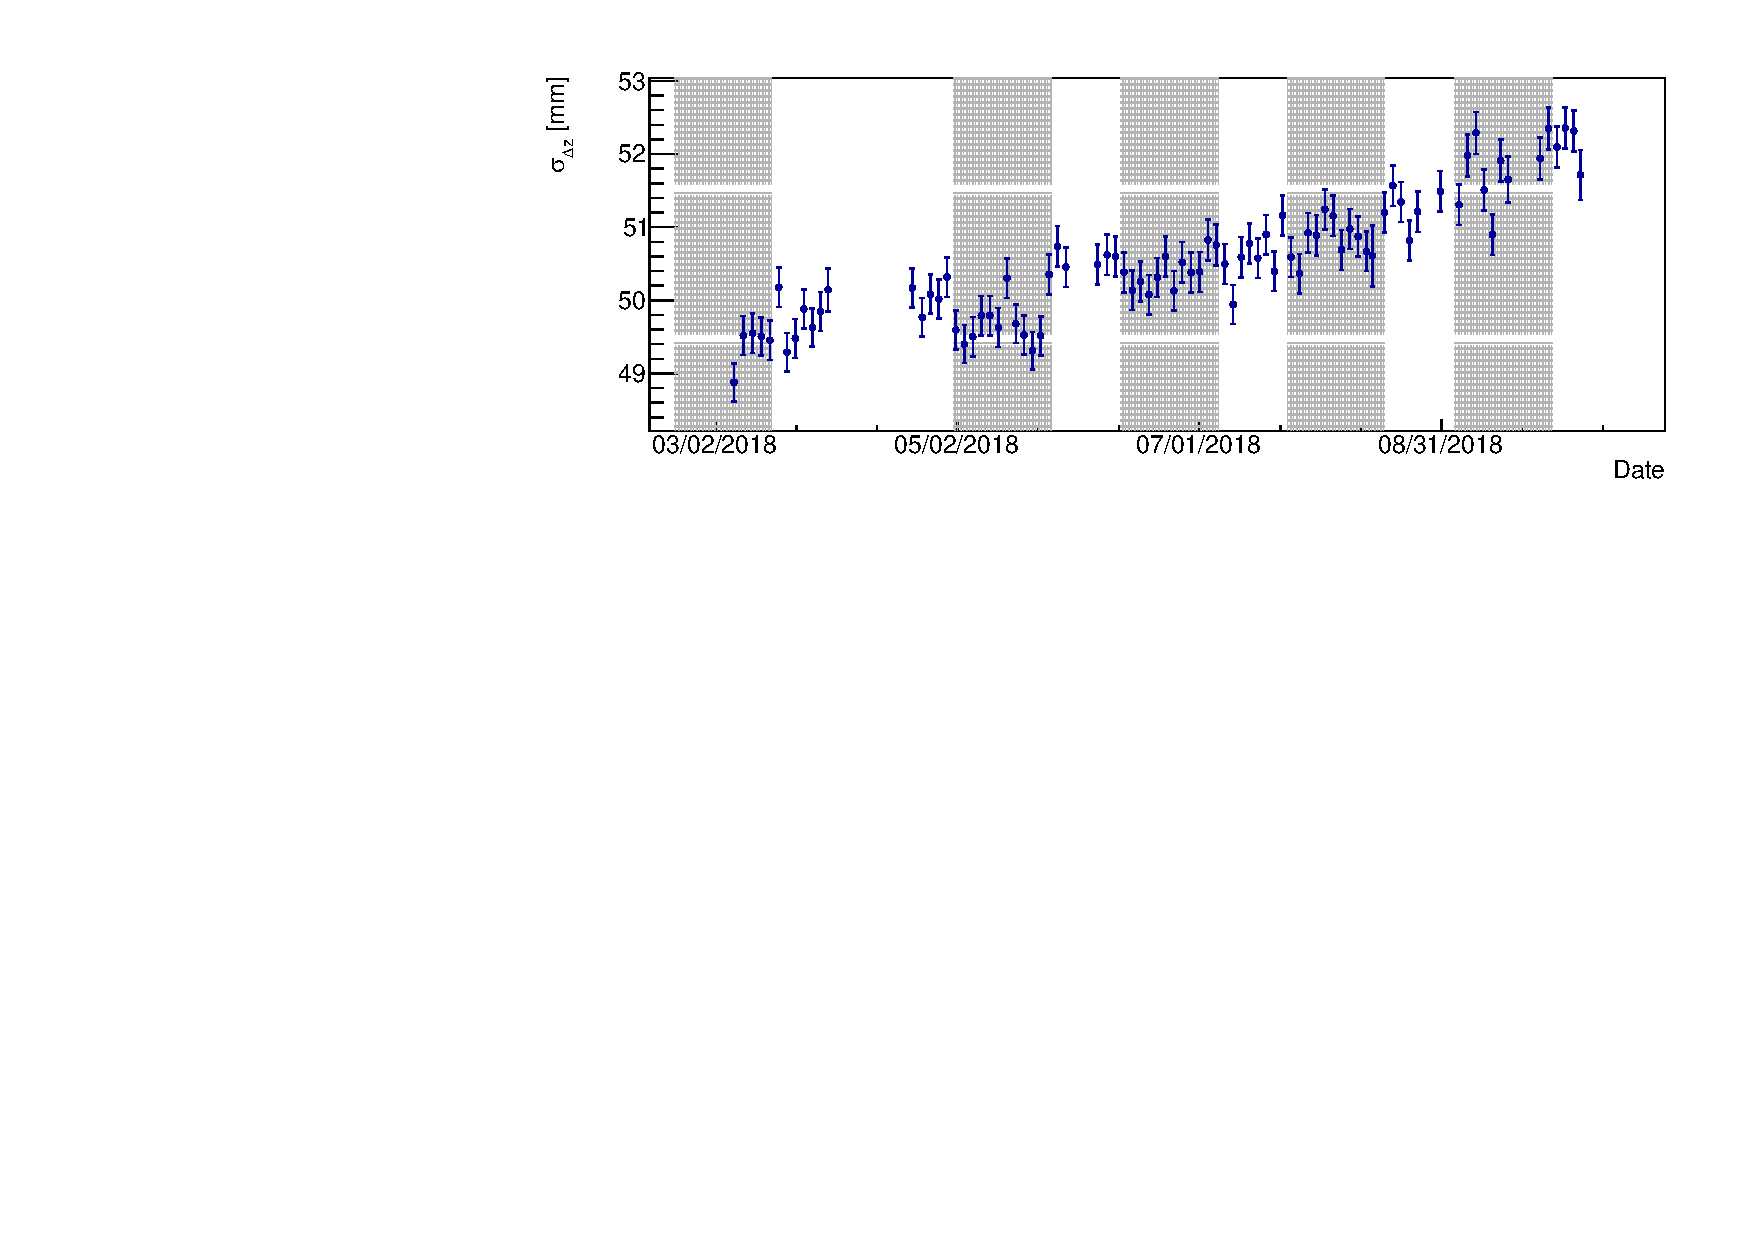
\includegraphics[width=0.9\linewidth]{tex/6-ac227-images/DetPerformance/RnPoDzSigmaVsTime}
	\caption{1$\sigma$ width of the $\Delta z$ distribution versus time. Shaded areas are reactor on periods.}
	\label{fig:rnpodzsigmavstime}
\end{figure}

Features of the \Po distribution are also useful to compare stability between segments. 
Figure~\ref{fig:histsvsseg} shows the distributions of the \Po energy, energy resolution, position, and position resolution in all individual segments. 
For Hamamatsu segments the energy scale and resolution are identical between segments to within $\sim \pm$0.25\% and $\sim \pm$6.5\% respectively. 
The ET segments vary more than the Hamamatsu segments, but for the case of the IBD analysis these segments are considered outside of the fiducial volume.

The position of events, $z$, was reconstructed individually for each cell by a combination of differences in timing and light yield between the two PMTs. 
As a result, the reconstructed $z$-position may vary from cell to cell. 
The relative alignment of the reconstructed $z$-position between segments can be observed by looking at the distribution of the mean of the position distribution for all segments.
It can be seen that, for Hamamatsu segments, all position reconstructions were aligned within $\pm$7 mm. 
The width of the $\Delta z$ distributions in Hamamatsu segments have a segment-to-segment variation of $\sim \pm$4 mm.

\Ac has proven to be useful in tracking energy, energy resolution, position, and position resolution over time and between segments.
Though IBD events are characteristically very different from RnPo $\alpha$ events, in energy and spatial event topologies, these distributions help to provide limits on systematic errors applied to the IBD analysis due to changing resolution effects and position reconstruction.
They also provide useful cross-checks for the behavior of new variables, such as $E_{smear}$, and tracking calibration performance over time.

\begin{figure}[H]
	\centering
	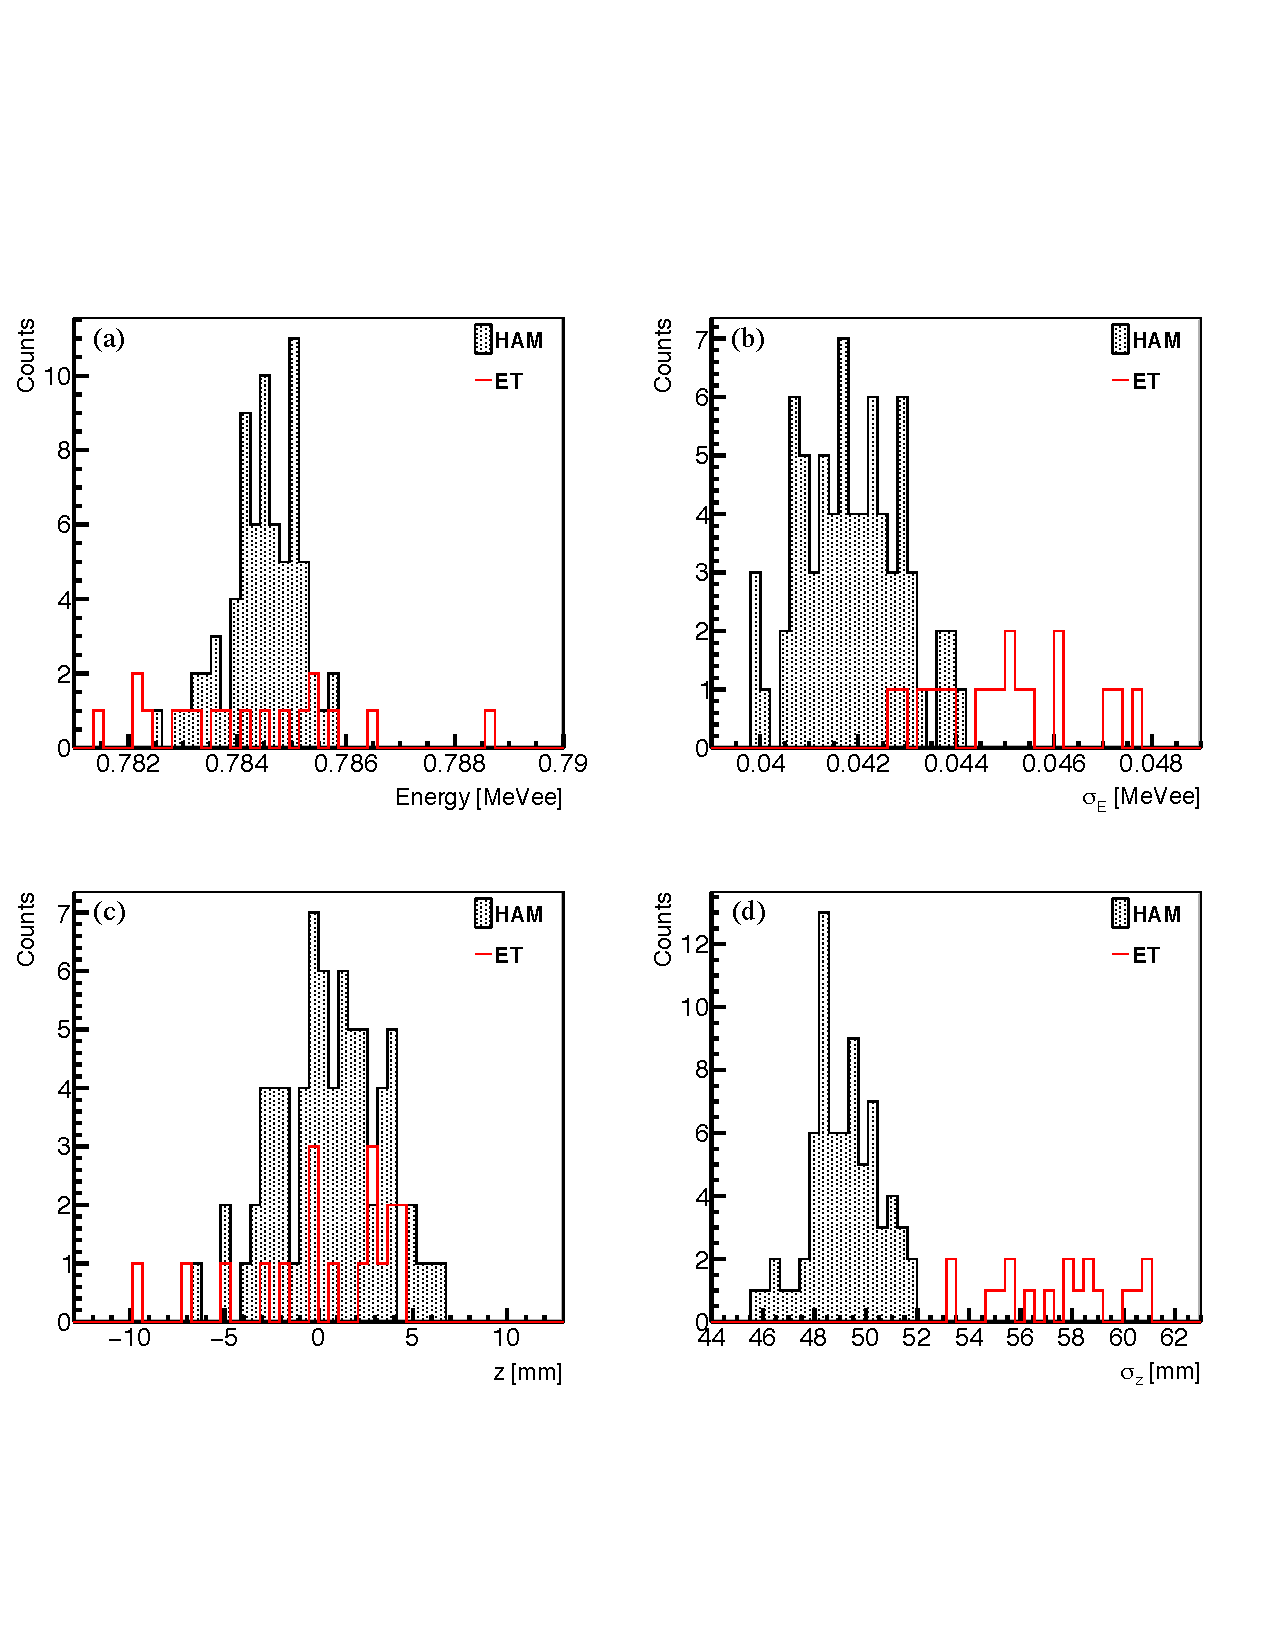
\includegraphics[width=1\linewidth]{tex/6-ac227-images/DetPerformance/HistsVsSeg}
	\caption{Segment-to-segment stability of the \Po energy (a), energy resolution (b), position reconstruction (c), and position resolution (d). Distributions are shown separately for Hamamatsu and ET segments.}
	\label{fig:histsvsseg}
\end{figure}

\subsection{\Ac Rate versus Time}

Observing the rate of \Ac in the AD over time provides a cross-check of the analysis while giving insight into the behavior of the detector.
Figure~\ref{fig:ratevstimefit} shows the \Ac rate measured versus time, integrated over all segments.
This was fit twice with an exponential of the form
\begin{equation}
	f(t) = R_0e^{\frac{-(t-t_0)\ln(2)}{t_{1/2}}}
	\label{eq:DtExp}
\end{equation}
where $R_0$ is allowed to vary both times and $t_{1/2}$, the half-life of \Ac (21.772~$\pm$~0.003~yrs), is fixed for one fit and allowed to vary in the other.
	
\begin{figure}[!b]
	\centering
	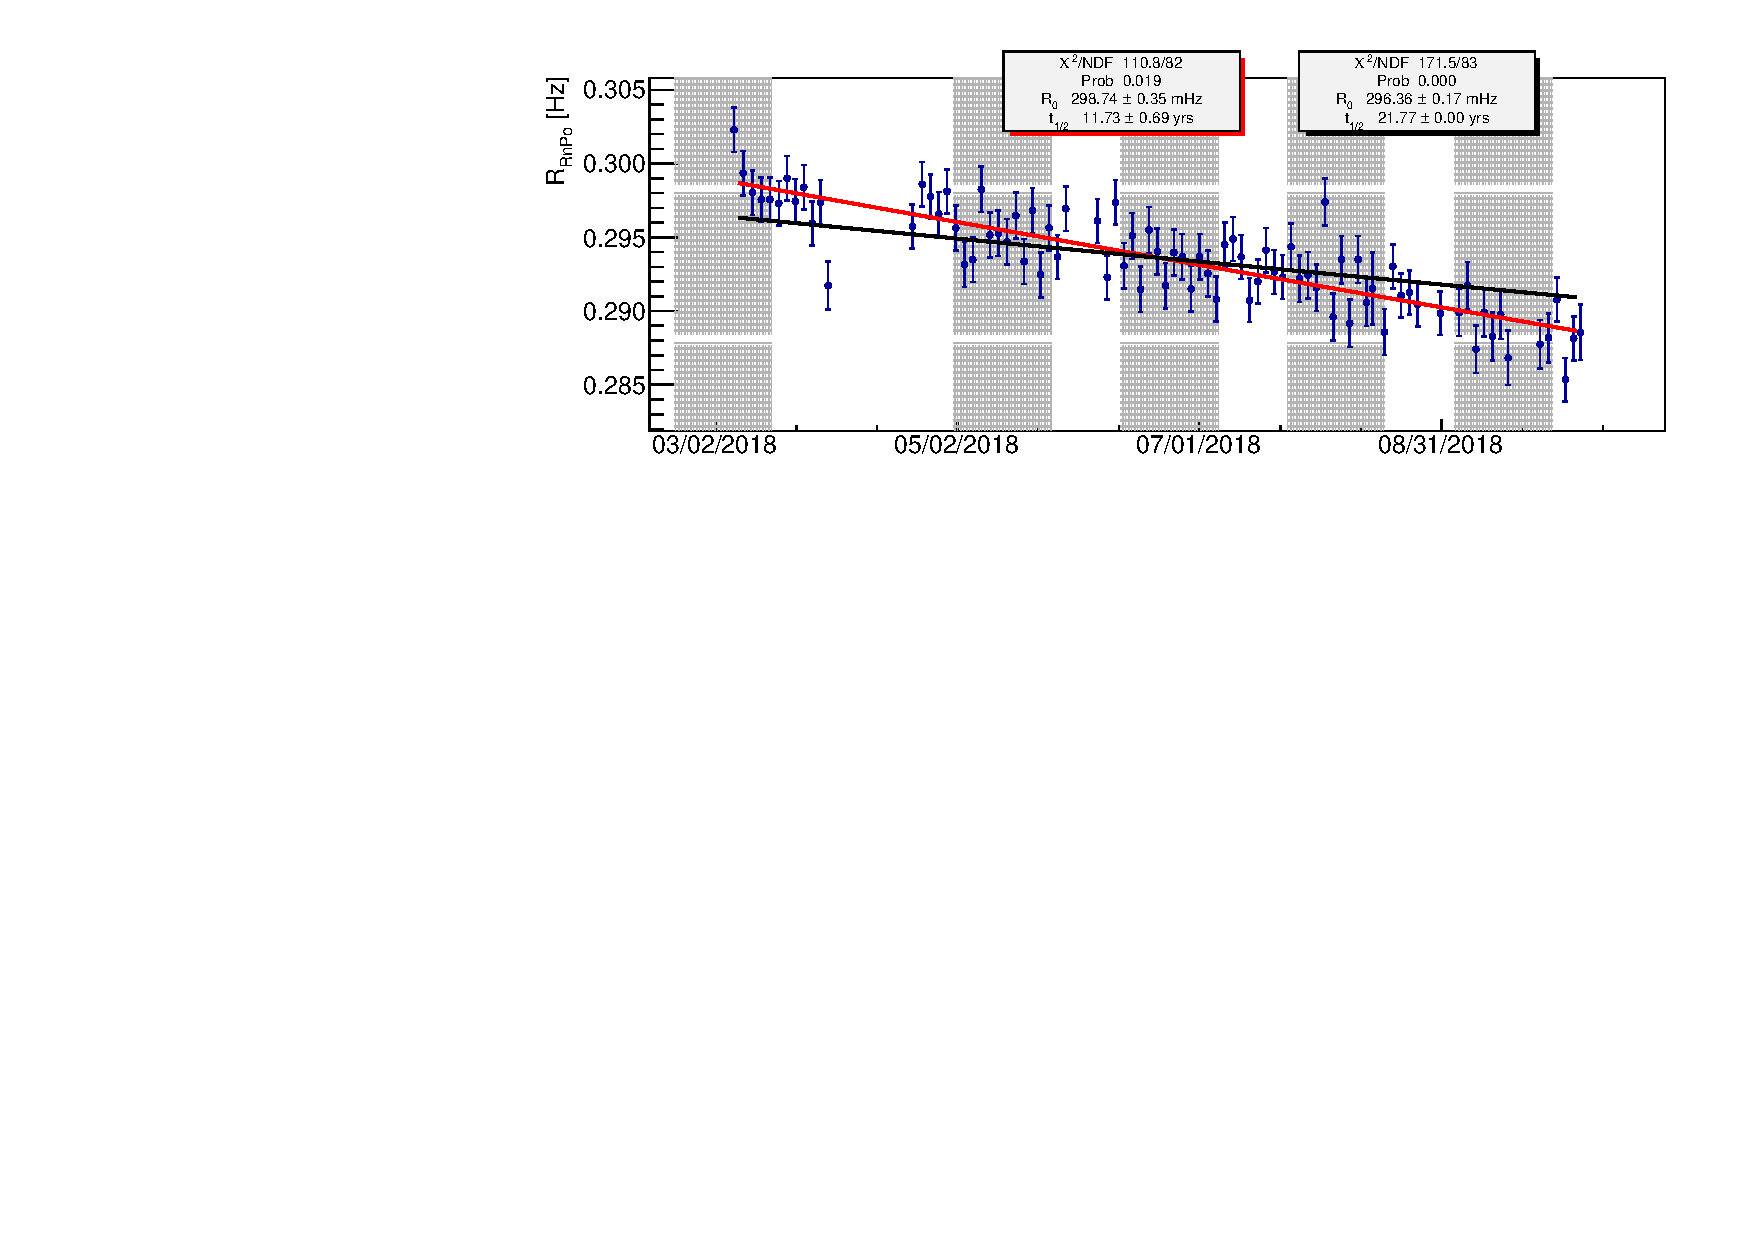
\includegraphics[width=1\linewidth]{tex/6-ac227-images/RateVsTime/RateVsTime_Fit}
	\caption{\Ac rate as measured versus time integrated over all segments. Fit with two exponentials, one in which the half-life of \Ac is allowed to vary (red) and one in which it is fixed (black). Errors are statistical. Shaded areas are reactor on periods.}
	\label{fig:ratevstimefit}
\end{figure}

When the half-life is allowed to vary, the fit returns a half-life of 11.73~$\pm$~0.69~yrs, suggesting that the measured rate of \Ac in the AD is falling 1.56 $\pm$ 0.21 \% faster than expectation over a period of 7 months.
The reason for this discrepancy is unclear.
Measurements of the \Po lifetime versus time, Figure~\ref{fig:lifetimevstime}, are consistent with its accepted lifetime, suggesting that the analysis is correctly accepting and measuring RnPo events.
The use of $\sigma$-based cuts for energy, PSD, and $\Delta z$ result in efficiencies that are always 99.9\% or higher, ruling out loss of events due to changing resolution as a solution.

One hypothesis is that \Ac is falling out of the LiLS solution. 
The process by which this would occur is unclear, but, in an attempt to gain more insight the detector was split into five sections of two rows each, as shown in Figure~\ref{fig:adsegmentsrows}.
The \Ac rate in each of these sections was measured and fit with the exponential in Equation~\ref{eq:DtExp}, allowing the half-life to vary.
See Figure~\ref{fig:ratevstimerows} for the rates and fits, and Figure~\ref{fig:achalflifevsrow} for the half-lives from the fit results versus row.

Though these results are statistics limited, a gradient from top to bottom can be seen in which the half-life gets shorter as one moves to the top of the detector.
This could be a sign of \Ac falling out of solution and sinking to the bottom of the detector.
The process by which this would happen, though, is unclear.
It is also not understood if it would sink in each individual segment, in which case a gradient might not be measured, or if it would all sink to the bottom.

In any case, the fact that the measured \Ac rate deviates from expectation indicates that it is not a clear proxy for a relative segment-to-segment volume measurement.
To account for this a 1\% systematic error should be applied to the segment-by-segment measured \Ac rates.

\begin{figure}[h]
	\centering
	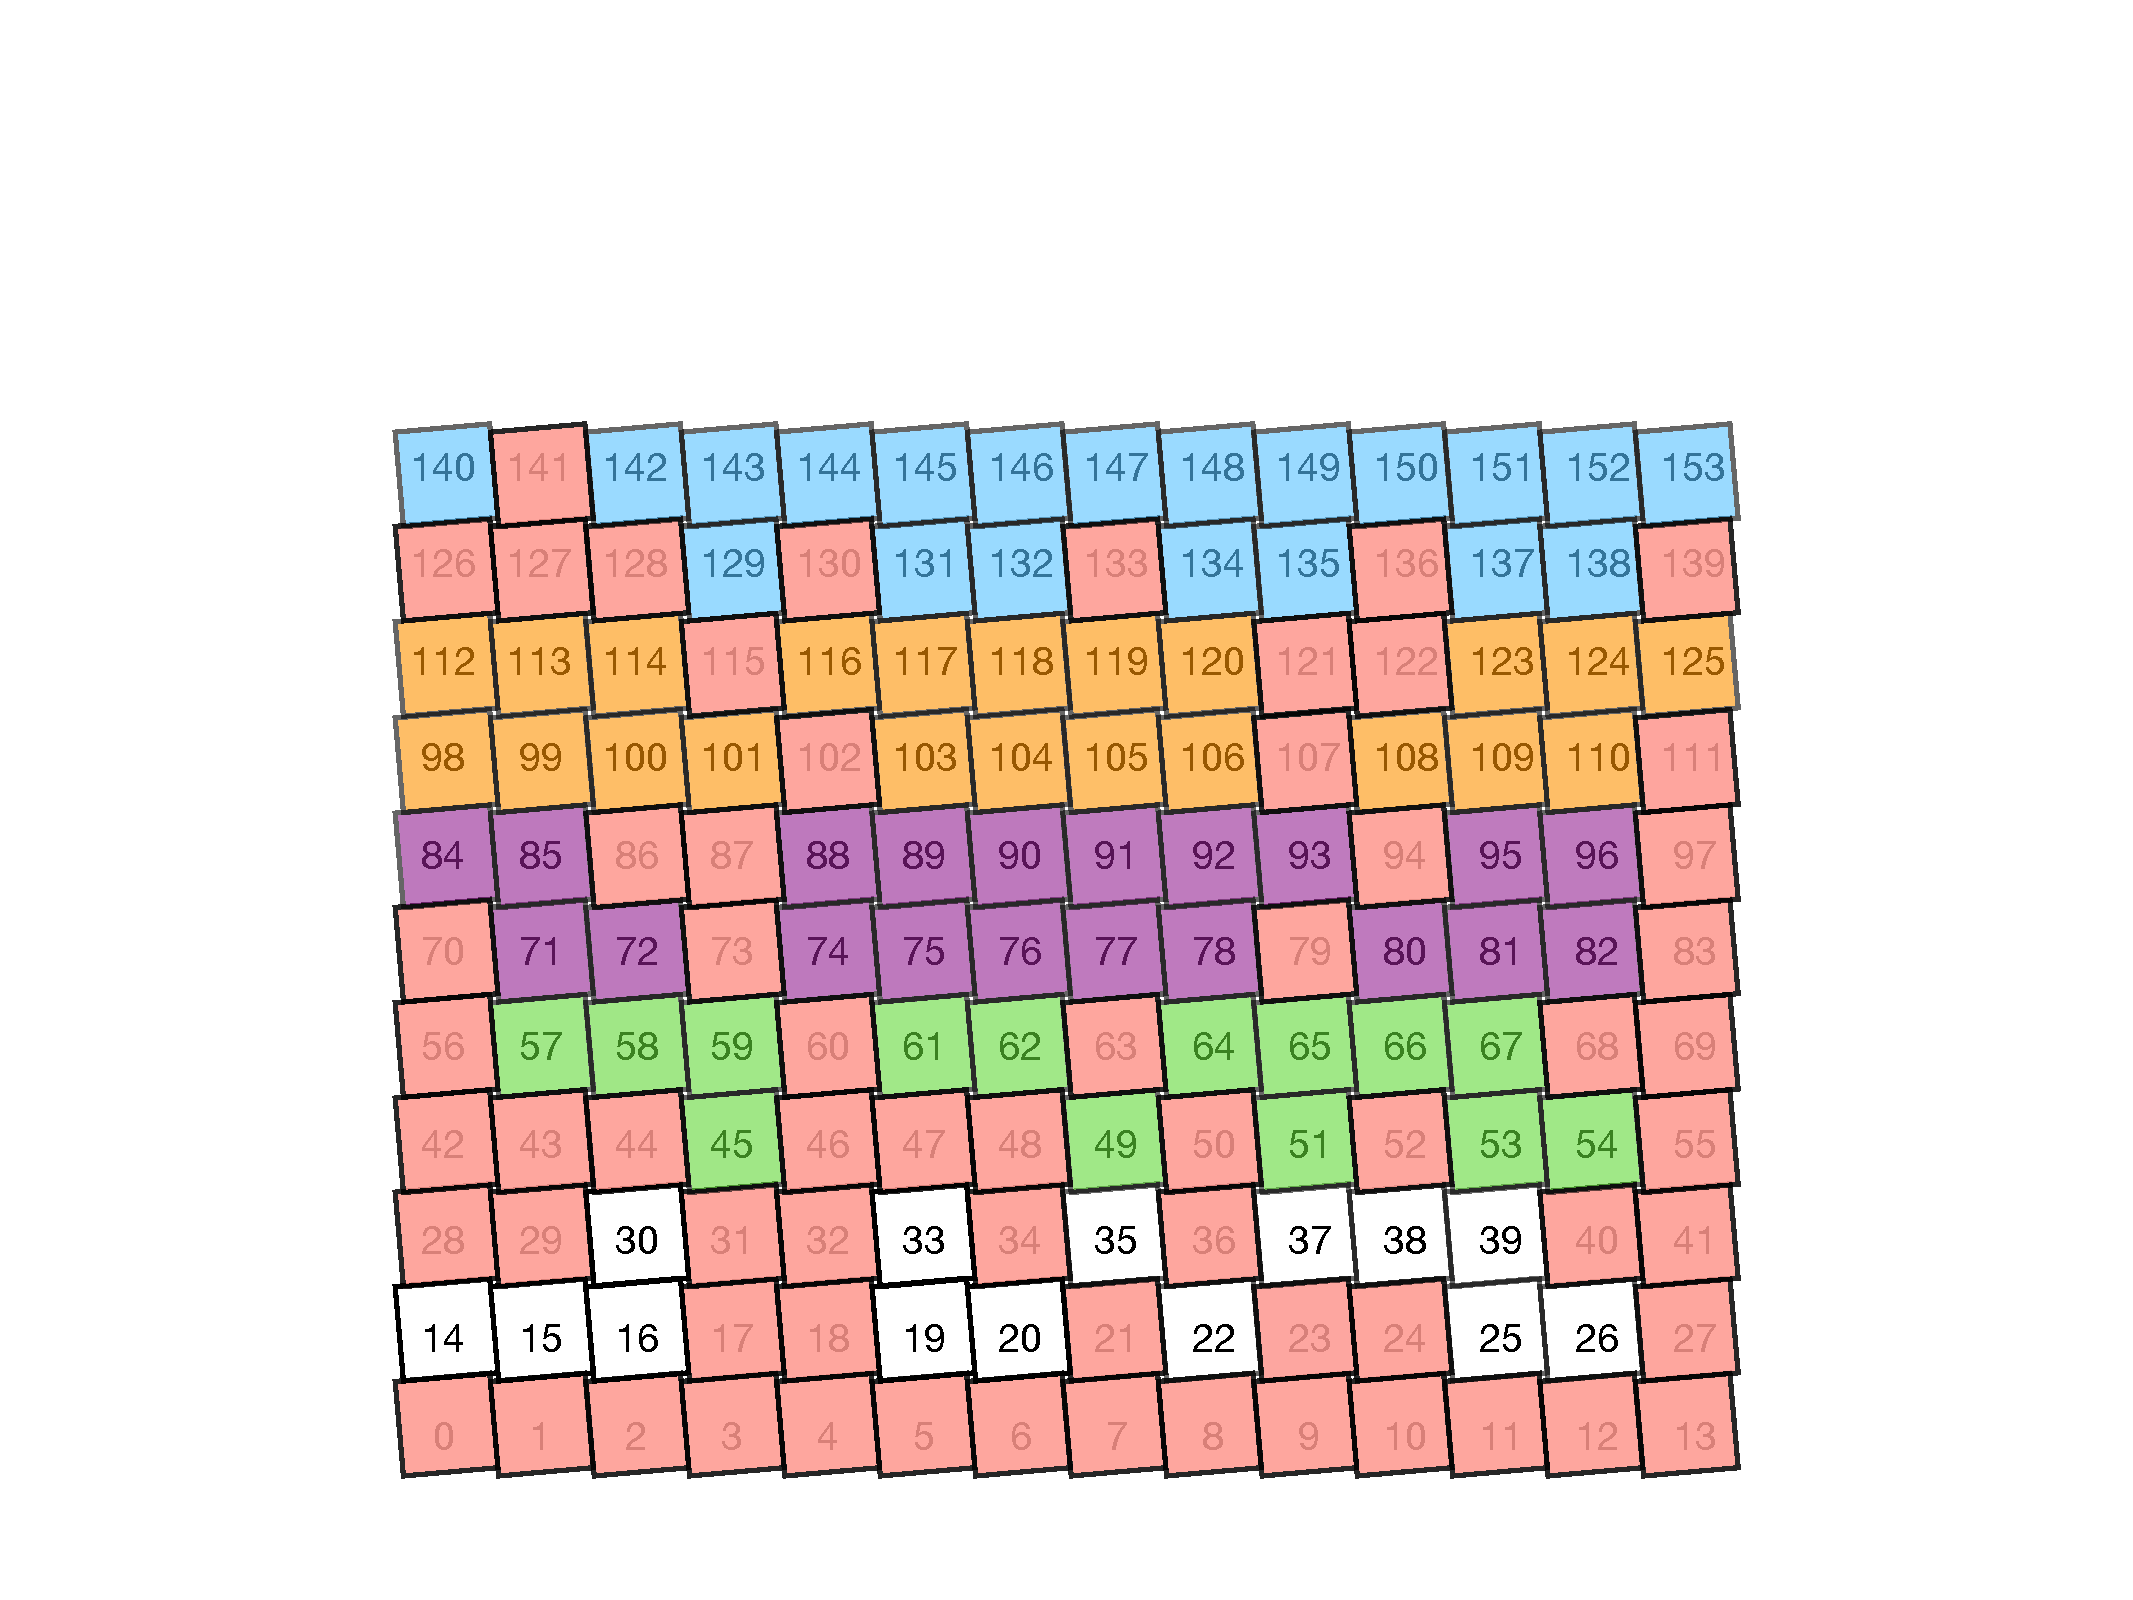
\includegraphics[width=0.5\linewidth]{tex/6-ac227-images/RateVsTime/AD_Segments_Rows}
	\caption{The PROSPECT detector divided into five sections of two rows each. Segments shaded in red are excluded from this analysis.}
	\label{fig:adsegmentsrows}
\end{figure}

\begin{figure}[H]
	\centering
	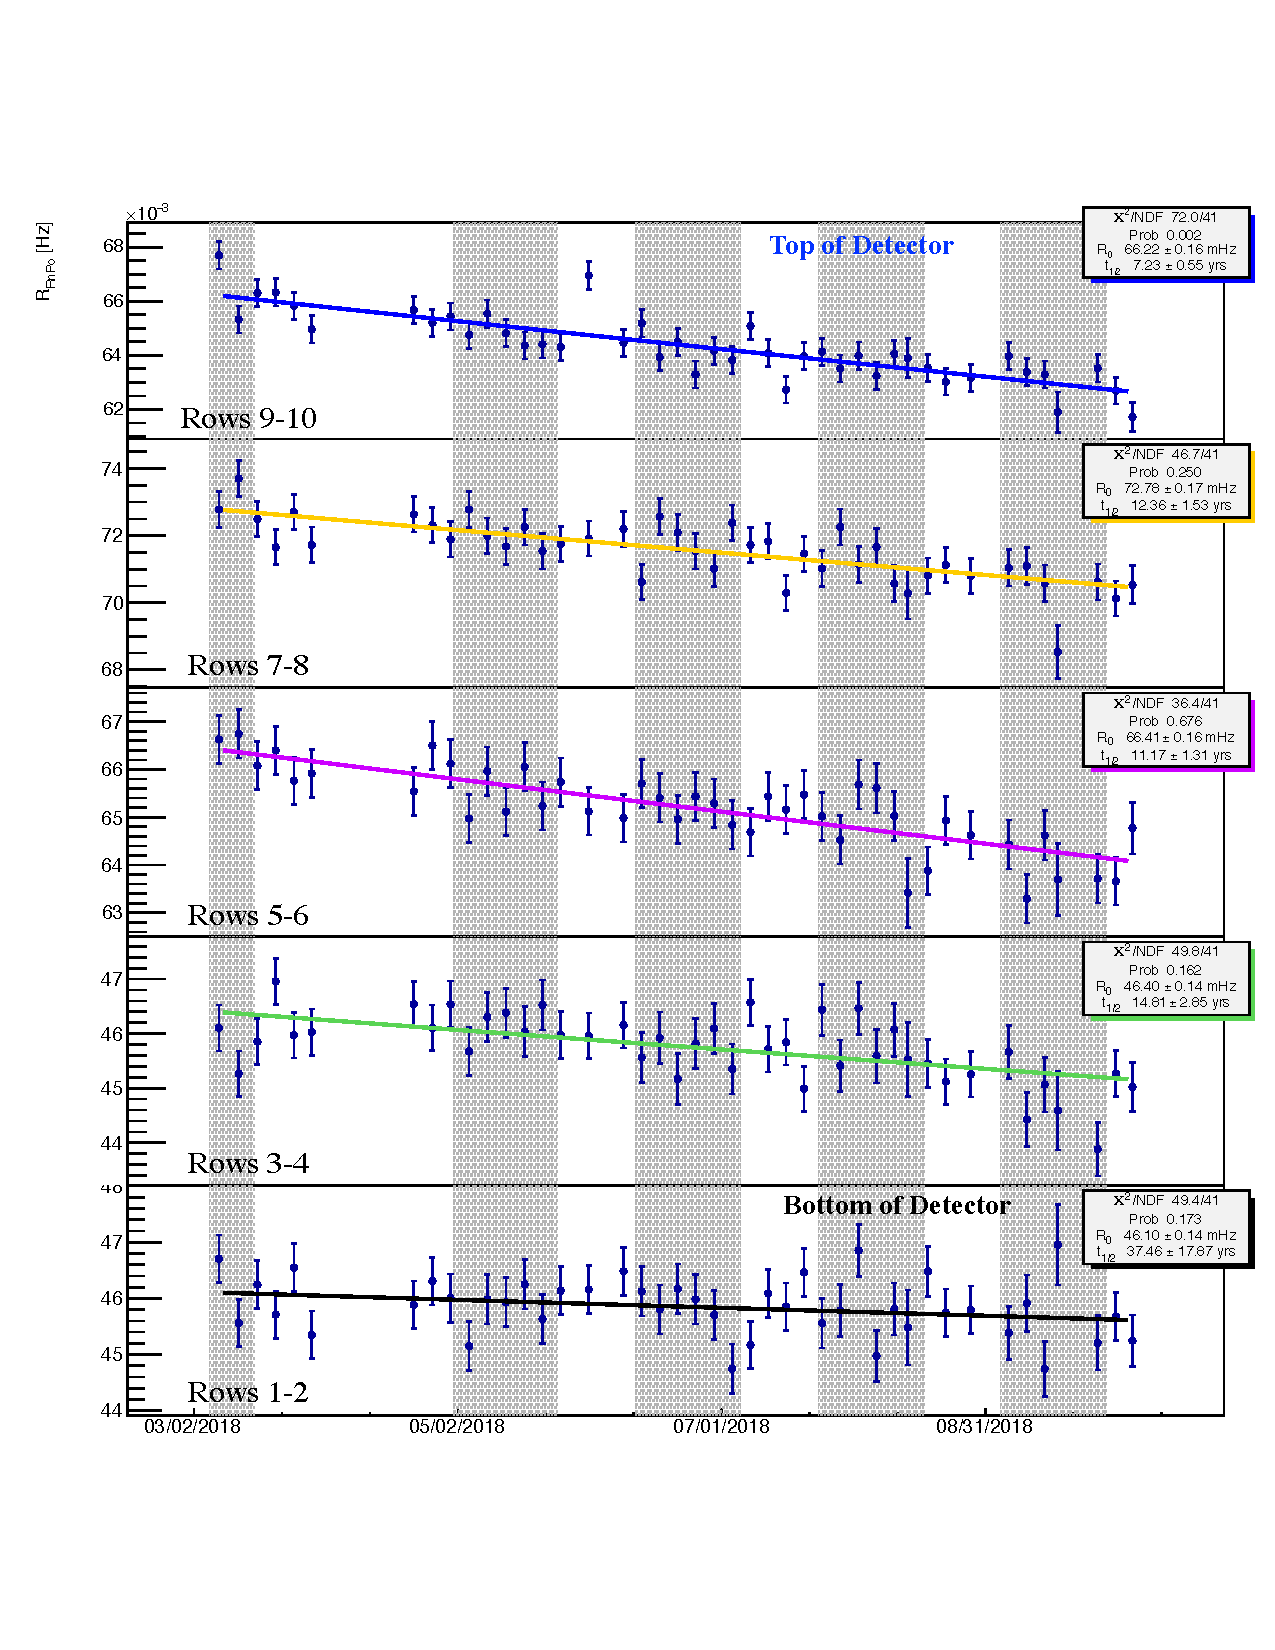
\includegraphics[width=0.87\linewidth]{tex/6-ac227-images/RateVsTime/RateVsTime_Rows_edit}
	\caption{The measured \Ac rate versus time for each section of two rows, fit with an exponential in which the half-life is allowed to vary.}
	\label{fig:ratevstimerows}
\end{figure}

\begin{figure}[H]
	\centering
	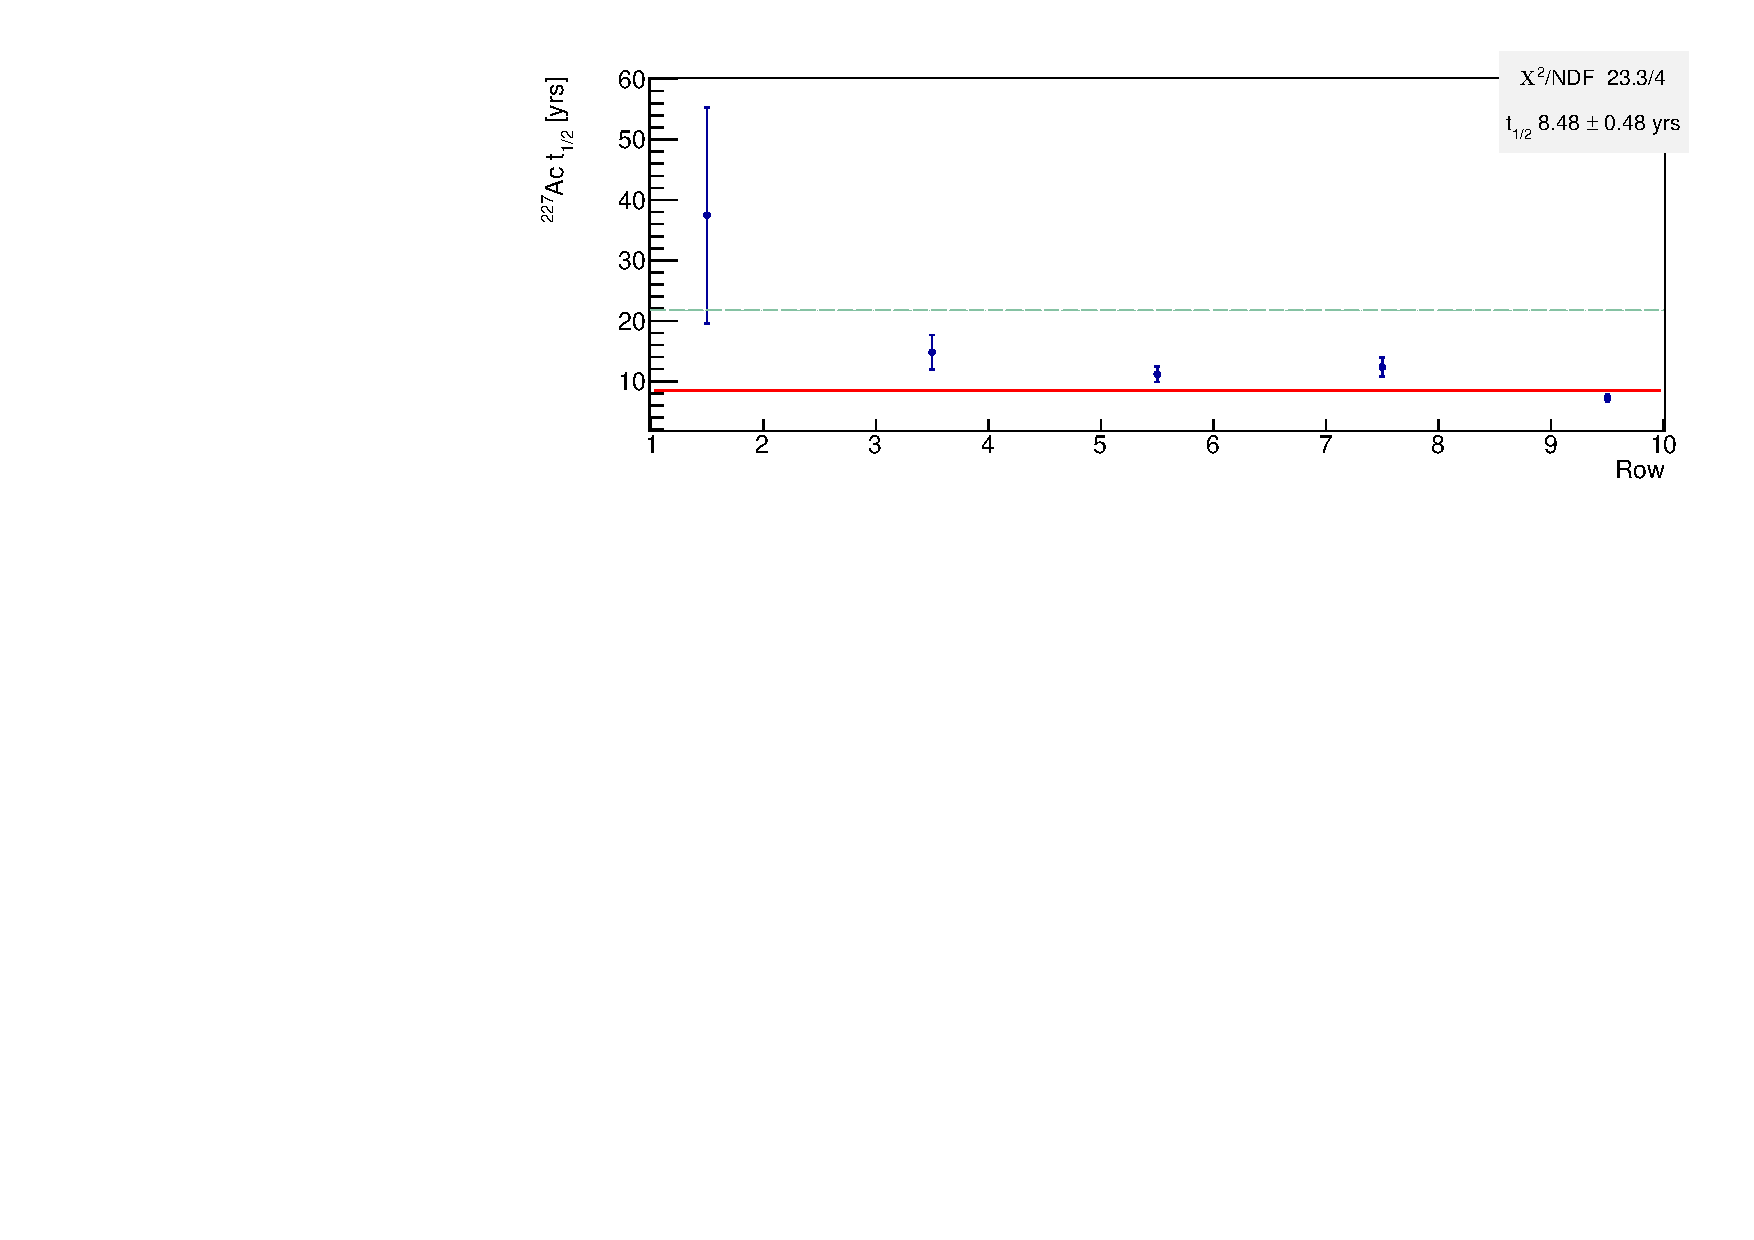
\includegraphics[width=0.8\linewidth]{tex/6-ac227-images/RateVsTime/AcHalfLifevsRow}
	\caption{The half-life results from fitting the \Ac rate versus time for five sections of two rows as shown in Figure~\ref{fig:ratevstimerows}.}
	\label{fig:achalflifevsrow}
\end{figure}



\subsection{\Ac Rate in Individual Segments}

The measured \Ac rate in each segment can be seen in Figure~\ref{fig:ratepercell}. 
Statistical errors for each segment are around 0.6\%.
The average rate, including Hamamatsu and ET segments, is 3.262 $\pm$ 0.002 mHz, in line with the expected factor of 3 less than the desired 0.01 Bq/cell.
The majority of segments vary $\pm$1\% from the average. 

The most glaring outliers are the top row, which are $\sim$1.5\% below average. 
A possible explanation for this is that the top row is not completely filled with scintillator, but the reason for these lower rates is unclear.

If the focus is shifted to only Hamamatsu segments, the fiducial segments, the average is found to be 3.270 $\pm$ 0.002 mHz.
The measured \Ac rates in all fiducial segments agree to within $\pm$2\%.
A histogram of the individual segment rates is shown in Figure~\ref{fig:histratepercell}.
The standard deviation of only the Hamamatsu segments is 0.026 mHz.

\begin{figure}[h]
	\centering
	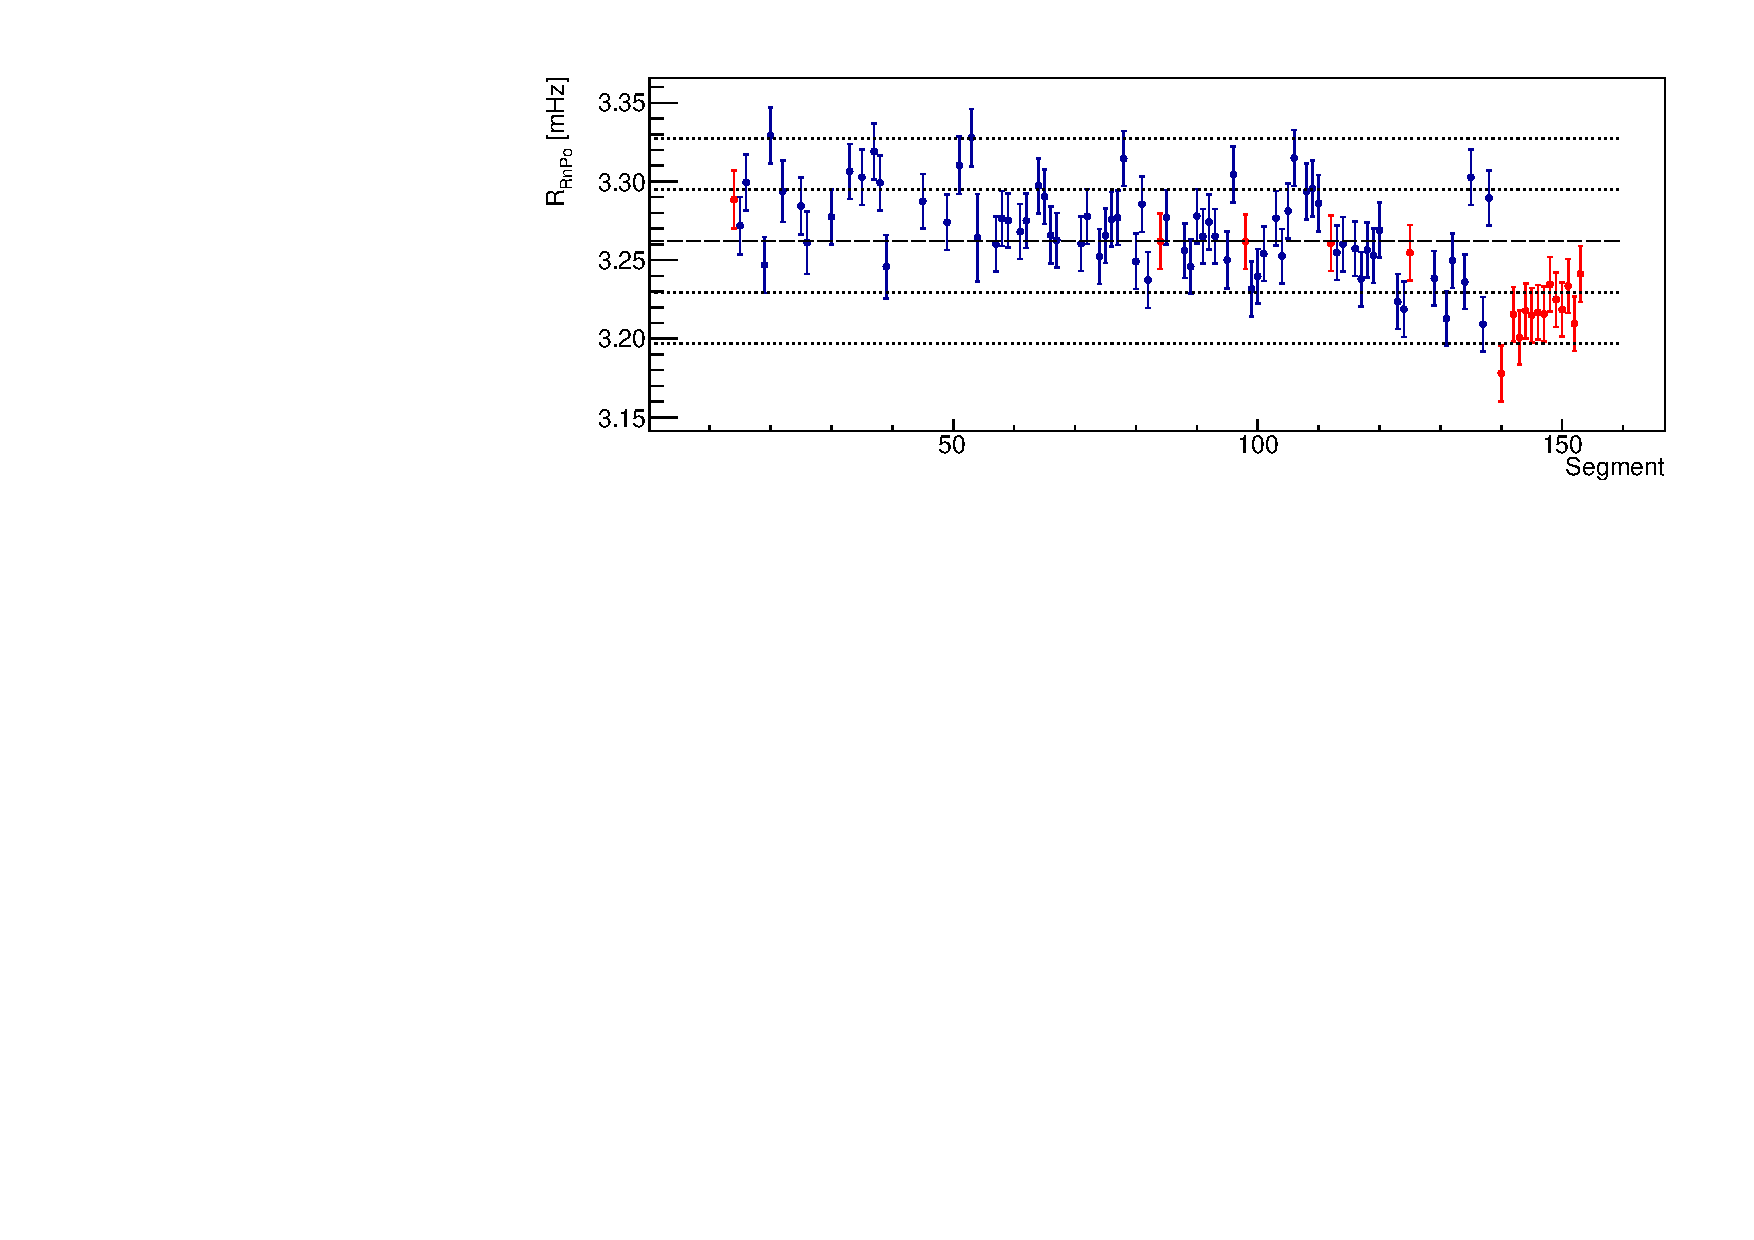
\includegraphics[width=1\linewidth]{tex/6-ac227-images/RatePerSeg/RatePerCell}
	\caption{The \Ac per individual segment integrated over all time. Dashed line represents the average over all segments. Dotted lines are $\pm$1\% and $\pm$2\% from the average. Blue: Hamamatsu segments, red: ET segments. Errors are statistical.}
	\label{fig:ratepercell}
\end{figure}

\begin{figure}[H]
	\centering
	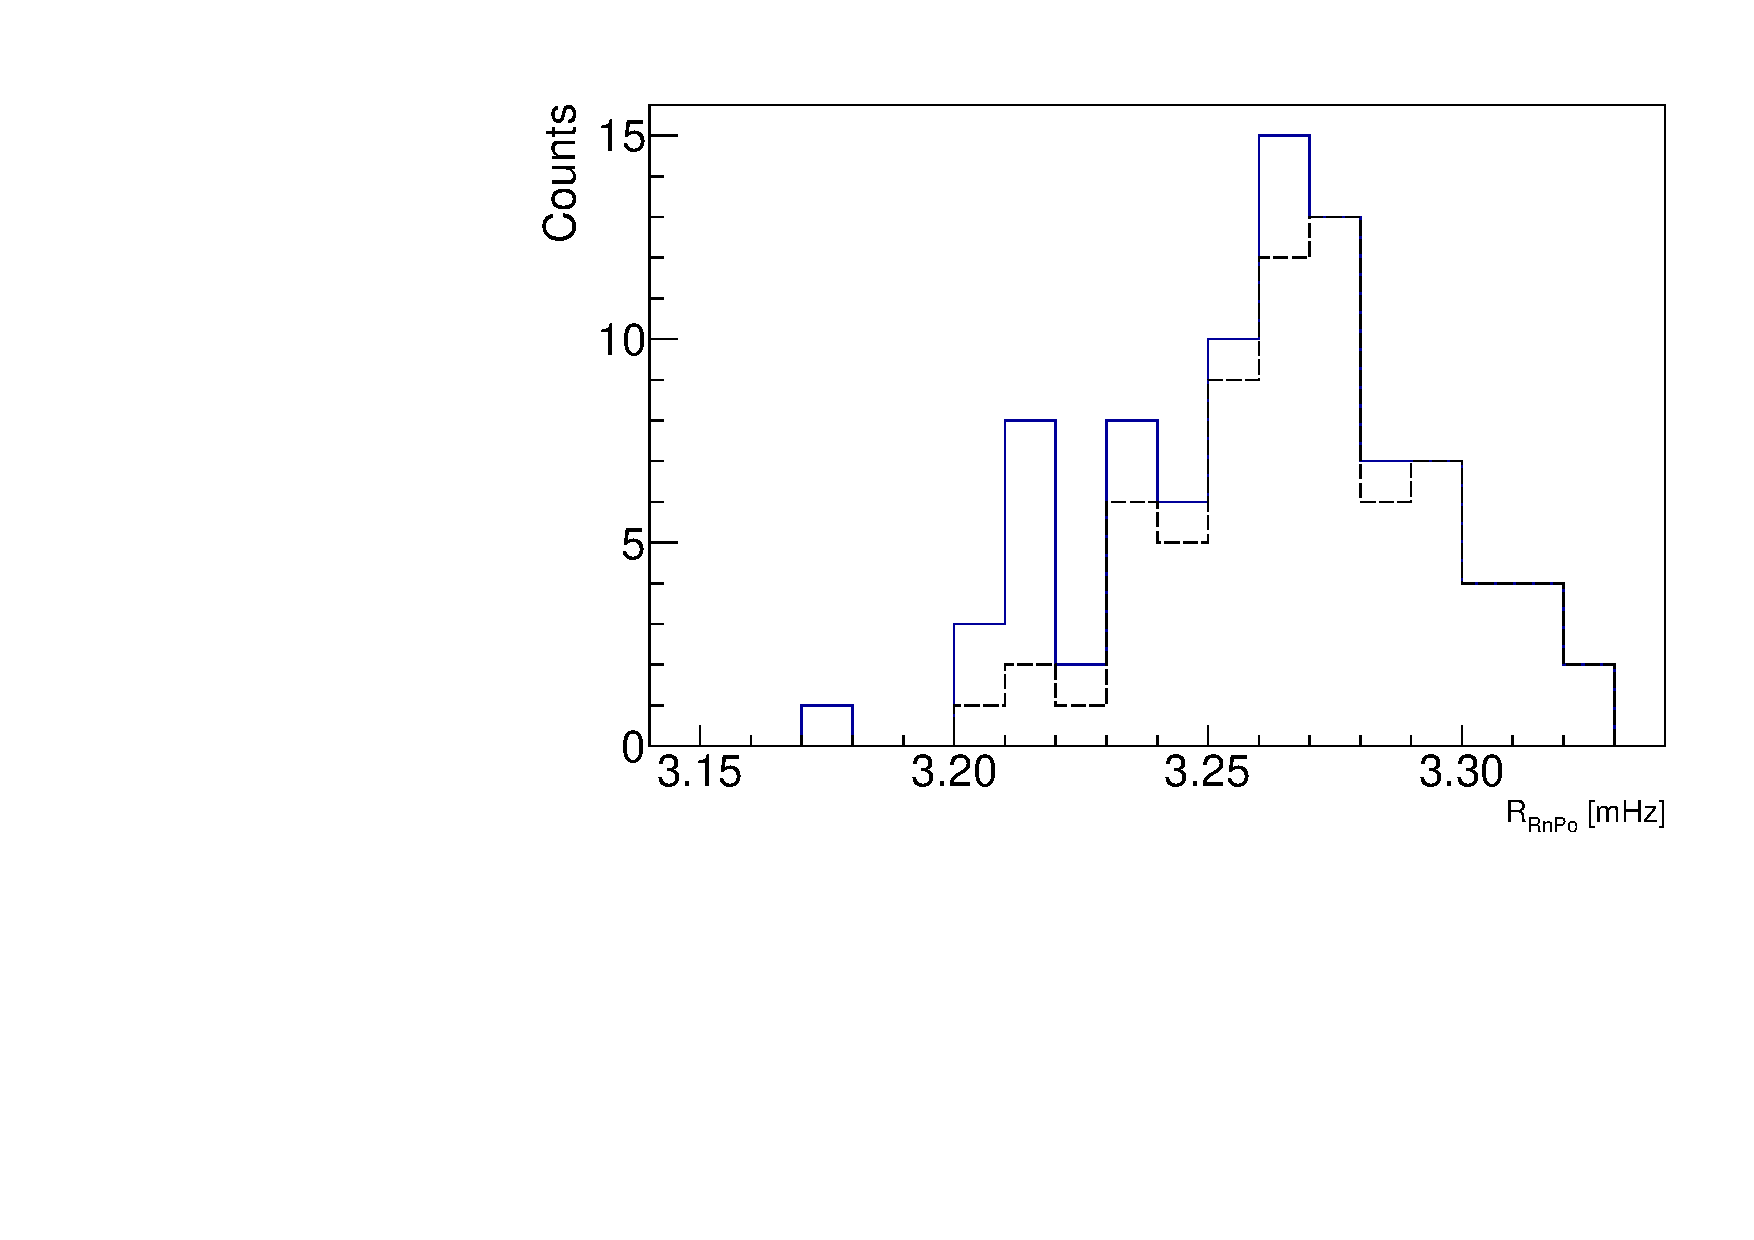
\includegraphics[width=0.7\linewidth]{tex/6-ac227-images/RatePerSeg/HistRatePerCell}
	\caption{Histogram of the individual segment \Ac rates. Blue (solid): Hamamatsu and ET segments, StdDev = 0.031 mHz. Black (dashed): only Hamamatsu segments, StdDev = 0.026 mHz.}
	\label{fig:histratepercell}
\end{figure}



\subsection{Systematic Errors}

Systematic uncertainties in this analysis come from three sources:
(i) the \Ac rate is falling faster than expectation (for this a 1\% systematic is applied), (ii) the energy, PSD, and $\Delta z$ cut efficiencies are calculated by assuming that all distributions are true Gaussians (for this a 0.15\% error is assigned), and (iii) the presence of other coincident alpha decays in the background that could contaminate the RnPo selection (for this a 0.22\% error is assigned).
It should be noted that up to this point only statistical errors have been presented. 
The systematic errors are never directly applied to the \Ac rates until Section~\ref{sec:AcBaseRates}, in which they are used to visualize how much relative rates as a function of distance from the reactor can vary.  

\subsubsection{Energy, PSD, and $\Delta$z Cuts}
In an effort to determine what level of systematic error to apply to the measured \Ac rates per segment a study was performed on the energy, PSD, and $\Delta z$ cuts.
For each cut (prompt and delay energy and PSD, and $\Delta$z) the width of the cut was changed from 2.5$\sigma$ about the mean to 4.0$\sigma$ in steps of 0.5$\sigma$ with the exception of an added step at 3.8$\sigma$.
The rate per segment was calculated for each of these instances and compared to the rate per segment when all cuts were at 4.0$\sigma$.
An example of the calculated rate per segment when the delayed energy cut is changed in this way can be seen in Figure~\ref{fig:ratevscelldelayecut}. 

For each segment and each cut, the quantity 
\begin{equation}
\frac{R_{4\sigma} - R_{i\sigma}}{R_{4\sigma}}
\label{eq:Sys}
\end{equation}
is calculated, where $R_{4\sigma}$ is the rate when a 4$\sigma$ cut is used and $R_{i\sigma}$ is the rate when a i$\sigma$ cut is used where (i: 2.5, 3.0, 3.5, 3.8).
This process was completed for the total data set and for a simulation set.
The simulation was done as an \Ac source dissolved in the scintillator in the AD with no reactor or ambient background.
The distributions of these results for data can be seen in Figure~\ref{fig:CutSys}.

\begin{figure}[!b]
	\centering
	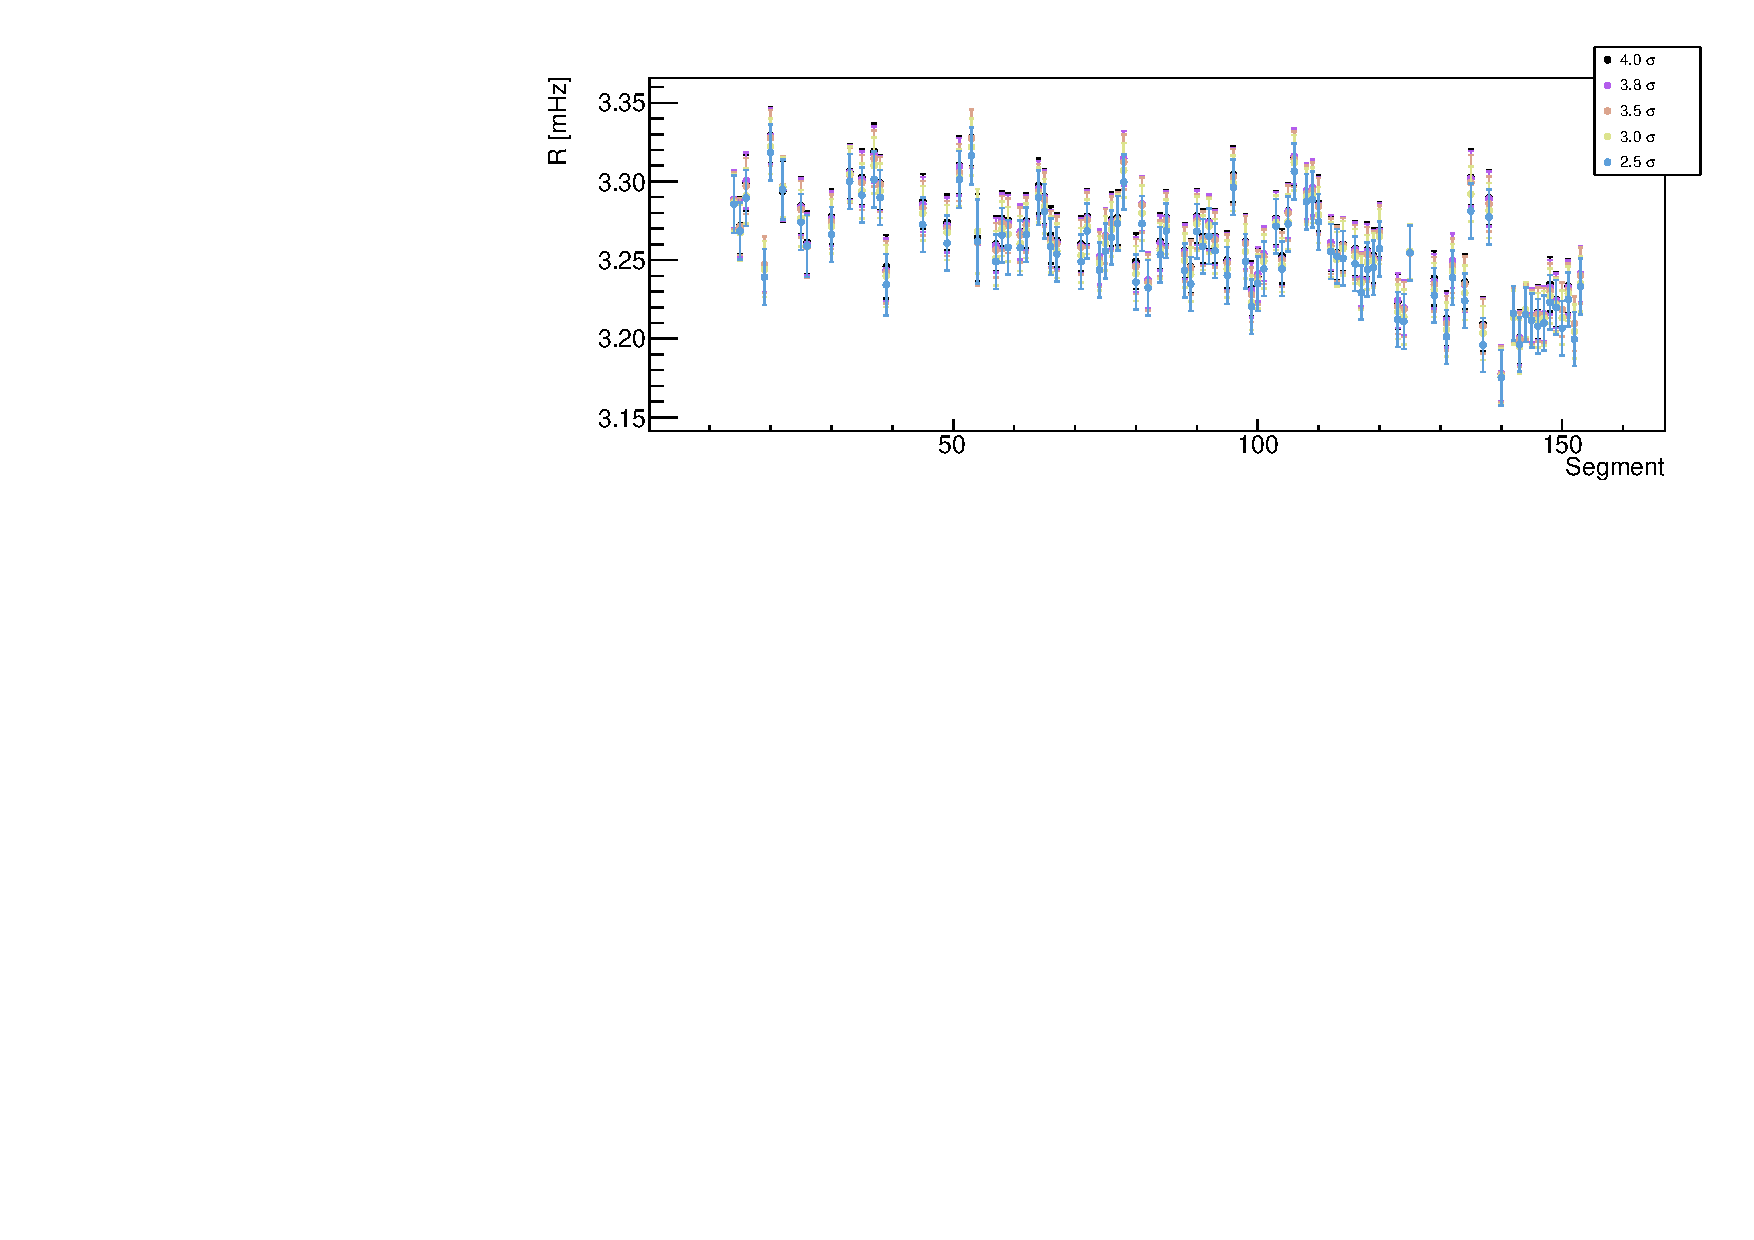
\includegraphics[width=1\linewidth]{tex/6-ac227-images/Systematics_Cuts/RateVsCell_DelayECut}
	\caption{\Ac rate per segment for different $\sigma$-based cuts on the delayed energy.}
	\label{fig:ratevscelldelayecut}
\end{figure}

The mean of each of these distributions is found and plotted according to the $\sigma$ cut used in Figure~\ref{fig:cutstudyresults}. 
The simulation results are shown in the same figure.
It can be seen that the mean of all distributions converge to zero at 4$\sigma$ with the maximum change in rate being $\sim$0.6 \% at 2.5$\sigma$.

If the method used to calculate efficiency was perfect (implying that all distributions are true Gaussians), then the rate would not depend on the $\sigma$ cut that is applied.
The results of this study show that this is not true and, therefore, a systematic error of 0.15\% will be applied to all measured \Ac rates per segment.

\begin{figure}[H]
	\begin{subfigure}{0.5\linewidth}
		\centering
		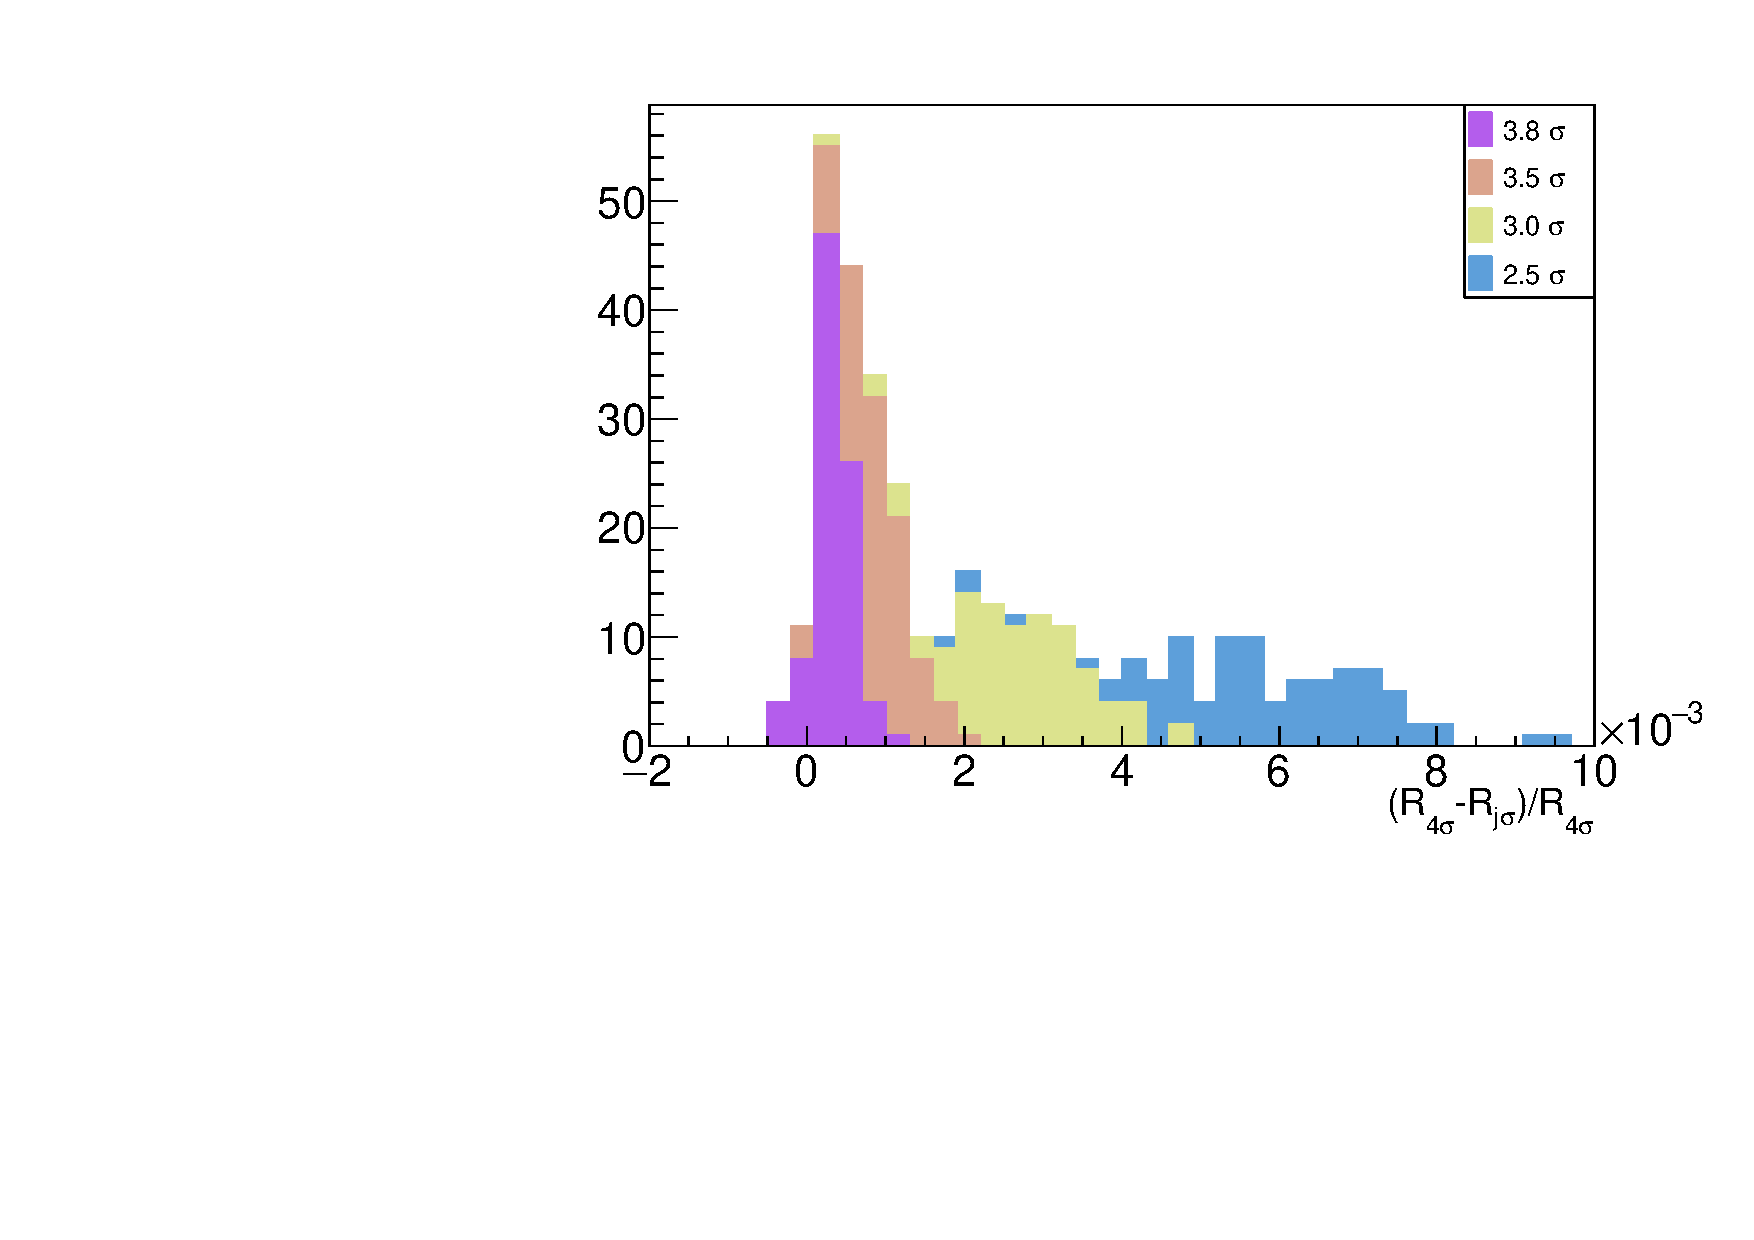
\includegraphics[width=0.85\linewidth]{tex/6-ac227-images/Systematics_Cuts/ResidVsCell_PromptECut}
		\caption{Prompt Energy}
	\end{subfigure}
	\begin{subfigure}{0.5\linewidth}
		\centering
		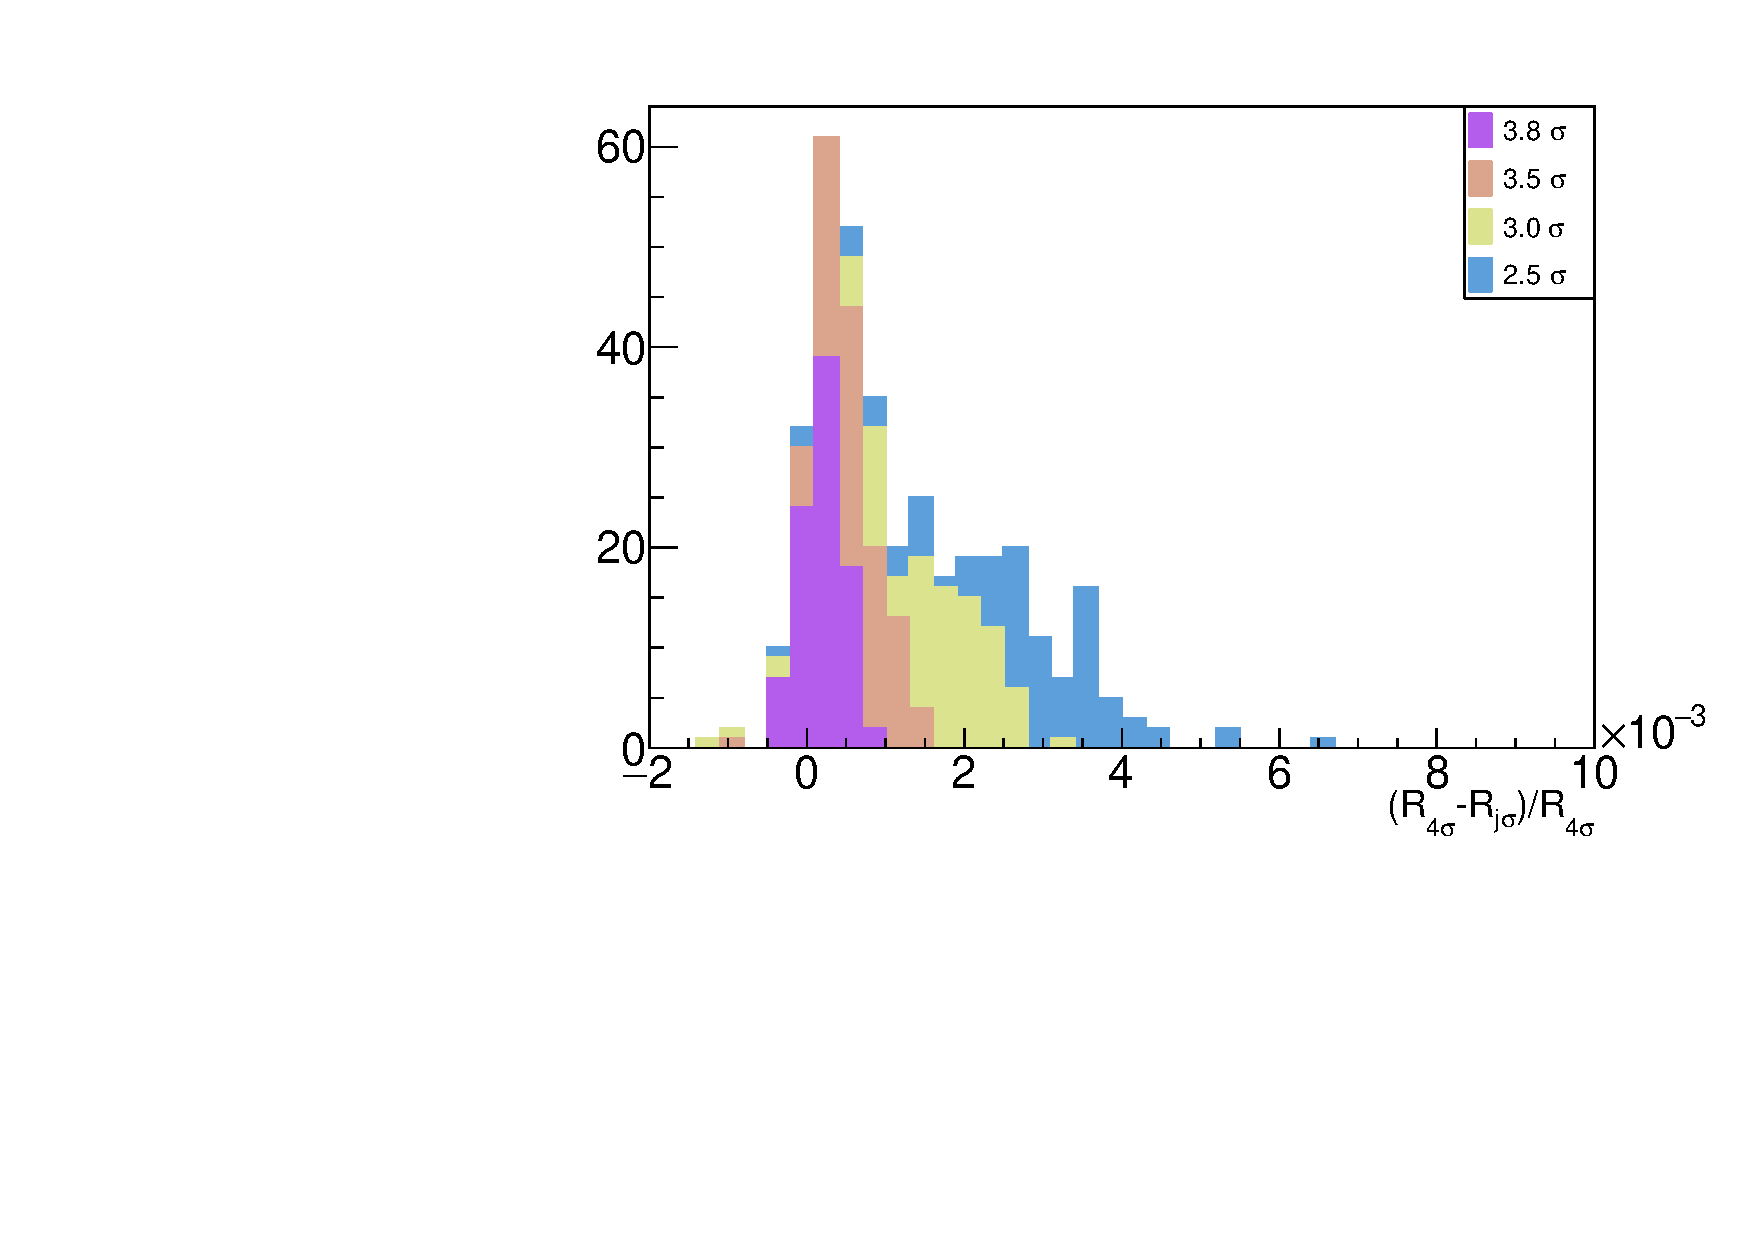
\includegraphics[width=0.85\linewidth]{tex/6-ac227-images/Systematics_Cuts/ResidVsCell_DelayECut}
		\caption{Delay Energy}
	\end{subfigure}
	\begin{subfigure}{0.5\linewidth}
		\centering
		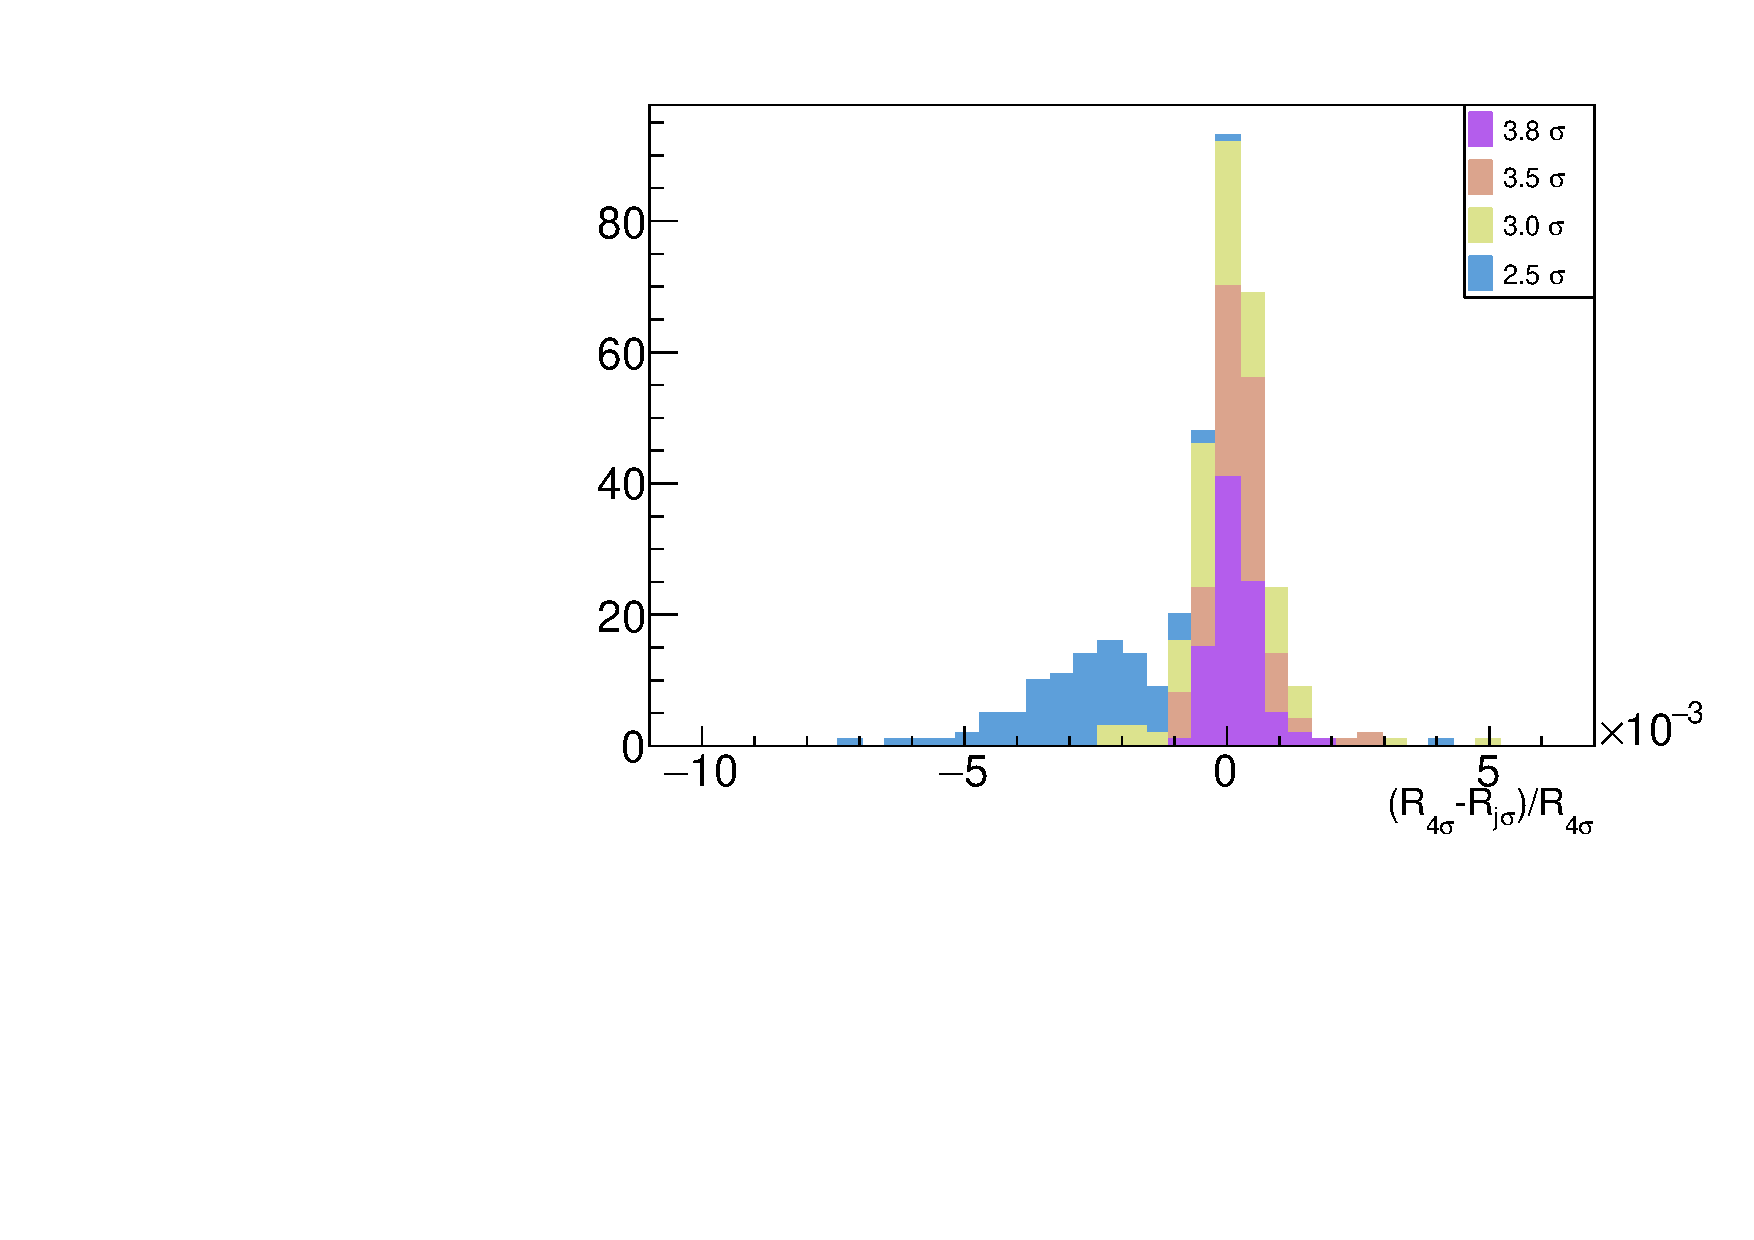
\includegraphics[width=0.85\linewidth]{tex/6-ac227-images/Systematics_Cuts/ResidVsCell_PromptPSDCut}
		\caption{Prompt PSD}
	\end{subfigure}
	\begin{subfigure}{0.5\linewidth}
		\centering
		\includegraphics[width=0.85\linewidth]{tex/6-ac227-images/Systematics_Cuts/ResidVsCell_DelayPSDCut}
		\caption{Delay PSD}
	\end{subfigure}
	\begin{subfigure}{1\linewidth}
		\centering
		\includegraphics[width=0.425\linewidth]{tex/6-ac227-images/Systematics_Cuts/ResidVsCell_DzCut}
		\caption{$\Delta$z}
	\end{subfigure}
	\caption{Pictured here are distributions created by calculating for each cell the difference between the rate using a given $\sigma$ cut and the rate using a 4$\sigma$ cut normalized by the rate using a 4$\sigma$ cut for data.}
	\label{fig:CutSys}
\end{figure}

\begin{figure}[H]
	\centering
	\includegraphics[width=0.8\linewidth]{tex/6-ac227-images/Systematics_Cuts/CutStudyResults}
	\caption{The mean of the distributions shown in Figure~\ref{fig:CutSys}. Solid lines: data. Dashed lines: simulation. Connecting lines are not fits; only meant to help guide the eye of the reader.}
	\label{fig:cutstudyresults}
\end{figure}

\subsubsection{Other Coincident Alphas}

There are two known event types with coincident alphas that occur in the PROSPECT AD that could contaminate the RnPo selection group. The first is an $\alpha$-$\alpha$ coincidence in the naturally occurring $^{232}$Th chain (the chain responsible for $^{212}$Bi$\rightarrow^{212}$Po (BiPo) events): $^{220}$Rn$\rightarrow ^{216}$Po$\rightarrow ^{212}$Pb. As listed in Table~\ref{tab:CoincAlpha}, the energy of these alphas fall in the selection range of the \Ac RnPo's (0.48/0.61-1.18 MeV) making it possible for them to be selected and not completely removed via the accidental subtraction.

The other possible event is the triple alpha decay in the \Ac chain: $^{223}$Ra$\rightarrow$\Rn$\rightarrow$\Po$\rightarrow ^{211}$Pb. 
Choosing an accidental background subtraction window that occurs before a given selected delay event (Po), in the time direction of the $^{223}$Ra contamination, helps to get rid of most of this contamination, but the rate of remaining events can be calculated.

Using the information found in Table~\ref{tab:CoincAlpha} and the time windows chosen for the \Ac RnPo selection it is possible to calculate the amount of contamination that is expected from these other alpha coincidences. 
Starting with the $^{232}$Th RnPo's, the fraction of $^{220}$Rn$\rightarrow ^{216}$Po alphas that are selected as `true' \Ac events, based on energy and time cuts, is $\sim$0.0061. 
If the rate of these events is approximated to be 0.085 Hz (based on a BiPo rate of 0.0547 Hz  \cite{Jones2800:2019}) then the rate of selection is $\sim$0.00052 Hz. 
If we approximate a total \Ac rate of 0.29 Hz, and therefore a rate of 0.24 Hz in the 0.5 - 12.845 ms time window used for selection, then the $^{232}$Th RnPo's will make up $\sim$0.22\% of the \Ac RnPo signal selection in the selection time window.
Therefore, a systematic error of 0.22\% will be applied.

The triple alpha in the \Ac chain contributes much less to the RnPo signal selection. Due to the nature of the background subtraction the probability that $^{223}$Ra$\rightarrow$\Rn coincident events pass both the energy cuts and the subtraction is 0.00083\%. No systematic error will be applied for these event types.

See Table~\ref{tab:CoincAlphaRate} for a summary of the energy and time cut efficiencies for both coincident alpha event types. 

\begin{table}[t]
	\centering
	\begin{tabular}{|c|c|c|c|c|}
		\hline 
		\textbf{Isotope} & \textbf{t$_{1/2}$ [ms]} & \textbf{E [MeV]} & \textbf{QE [MeVee]} & \textbf{1$\sigma$ width [MeVee] (5\% res.)} \\ 
		\hline 
		$^{220}$Rn & 55600 & 6.2881 & 0.5942 & 0.0412 \\ 
		\hline 
		$^{216}$Po & 145 & 6.7783 & 0.6776 & 0.0412 \\ 
		\hline \hline
		$^{223}$Ra & 9.88$\times$10$^{8}$ & 5.7162 & 0.5031 & 0.0355 \\ 
		\hline 
		$^{219}$Rn & 3860 & 6.8191 & 0.6847 & 0.0414 \\ 
		\hline 
		$^{215}$Po & 1.781 & 7.3861 & 0.7876 & 0.0444 \\ 
		\hline 
	\end{tabular} 
	\caption{Dominant $\alpha$ energies for coincident $\alpha$ event chains that could contaminate the \Ac RnPo signal. Also given are the quenched energies (QE) and 1$\sigma$ widths based on a 5\% energy resolution.}
	\label{tab:CoincAlpha}
\end{table}

\begin{table}[H]
	\centering
	\begin{tabular}{|c|c|c|c|c|c|}
		\hline 
		\textbf{Prompt} & \textbf{Delay} & \textbf{t$_{1/2}$ [ms]} & \textbf{Energy Cut Eff.} & \textbf{Time Cut Eff.} & \textbf{Rate [mHz]} \\ 
		\hline 
		$^{220}$Rn & $^{216}$Po & 145 & 0.925 & 0.0066 & 0.52  \\ 
		\hline 
		$^{223}$Ra & $^{219}$Rn & 3860 & 0.815 & 0.000010  & 0.0021 \\ 
		\hline 
	\end{tabular} 
	\caption{Energy and time cut efficiencies and resulting rates (assuming an \Ac rate of 240 mHz) for both coincident $\alpha$ event chains that could contribute to contamination of the \Ac RnPo signal selection.}
	\label{tab:CoincAlphaRate}
\end{table}


\subsection{\Ac Rates per Baseline} \label{sec:AcBaseRates}

The original goal of adding \Ac to the PROSPECT detector was to measure relative volume differences and apply these corrections to the oscillation analysis. 
The oscillation analysis is carried out by dividing the detector into baselines, or distances from the reactor core, and comparing the measured spectra between baselines.
A similar process can be done for the \Ac rates, and then corrections can be applied to the number of IBD counts versus baseline based on the \Ac results.

The detector was divided into 10 individual baselines, where baseline 1 is closest to the reactor core.
Figure~\ref{fig:adsegments} shows the configuration of baselines that was chosen for this data set.
The \Ac rate measured for each segment was then averaged over each baseline (error-weighted) and then plotted relative to the average rate in the first baseline.
The results of this can be seen in Figure~\ref{fig:fidratevsbaseline}.
Note that the rates used in this part of the analysis were measured using an additional $z$-fiducial cut of -448~$<~z~<$~448 mm, in order to use the same fiducial volume as the oscillation analysis.

It can be seen that the average rates vary less than 1\% over all baselines.
The statistics of this data set do not require volume corrections at this level, but these results provide a lower limit that could be applied to the oscillation analysis.\footnote{As the oscillation analysis for this data set is not yet completed, these results cannot currently be applied as corrections to the IBD rate versus baseline. 
Instead, the same analysis described in this chapter was applied to the data set used for the published oscillation results and corrections were applied accordingly, as described in the next chapter.}
For a data set with large statistics, in which volume variations could become an important systematic error, this method of adding \Ac and measuring the decay rates as a proxy for volume is proven to be effective.

\begin{figure}[!t]
	\centering
	\includegraphics[width=0.6\linewidth]{tex/6-ac227-images/Baseline/AD_Segments}
	\caption{The PROSPECT AD divided into 10 baselines, where baseline 1 is closest to the reactor. Segments in white are either fiducial segments or were turned off.}
	\label{fig:adsegments}
\end{figure}

\begin{figure}[h]
	\centering
	\includegraphics[width=0.9\linewidth]{tex/6-ac227-images/Baseline/FidRateVsBaseline}
	\caption{The \Ac rate for fiducial $z$ volume averaged over each of the 10 defined baselines and relative to the first baseline. Error bars are statistical, systematic errors are shown as the shaded region.}
	\label{fig:fidratevsbaseline}
\end{figure}





